% Options for packages loaded elsewhere
\PassOptionsToPackage{unicode}{hyperref}
\PassOptionsToPackage{hyphens}{url}
\documentclass[
]{article}
\usepackage{xcolor}
\usepackage[margin=1in]{geometry}
\usepackage{amsmath,amssymb}
\setcounter{secnumdepth}{-\maxdimen} % remove section numbering
\usepackage{iftex}
\ifPDFTeX
  \usepackage[T1]{fontenc}
  \usepackage[utf8]{inputenc}
  \usepackage{textcomp} % provide euro and other symbols
\else % if luatex or xetex
  \usepackage{unicode-math} % this also loads fontspec
  \defaultfontfeatures{Scale=MatchLowercase}
  \defaultfontfeatures[\rmfamily]{Ligatures=TeX,Scale=1}
\fi
\usepackage{lmodern}
\ifPDFTeX\else
  % xetex/luatex font selection
\fi
% Use upquote if available, for straight quotes in verbatim environments
\IfFileExists{upquote.sty}{\usepackage{upquote}}{}
\IfFileExists{microtype.sty}{% use microtype if available
  \usepackage[]{microtype}
  \UseMicrotypeSet[protrusion]{basicmath} % disable protrusion for tt fonts
}{}
\makeatletter
\@ifundefined{KOMAClassName}{% if non-KOMA class
  \IfFileExists{parskip.sty}{%
    \usepackage{parskip}
  }{% else
    \setlength{\parindent}{0pt}
    \setlength{\parskip}{6pt plus 2pt minus 1pt}}
}{% if KOMA class
  \KOMAoptions{parskip=half}}
\makeatother
\usepackage{color}
\usepackage{fancyvrb}
\newcommand{\VerbBar}{|}
\newcommand{\VERB}{\Verb[commandchars=\\\{\}]}
\DefineVerbatimEnvironment{Highlighting}{Verbatim}{commandchars=\\\{\}}
% Add ',fontsize=\small' for more characters per line
\usepackage{framed}
\definecolor{shadecolor}{RGB}{248,248,248}
\newenvironment{Shaded}{\begin{snugshade}}{\end{snugshade}}
\newcommand{\AlertTok}[1]{\textcolor[rgb]{0.94,0.16,0.16}{#1}}
\newcommand{\AnnotationTok}[1]{\textcolor[rgb]{0.56,0.35,0.01}{\textbf{\textit{#1}}}}
\newcommand{\AttributeTok}[1]{\textcolor[rgb]{0.13,0.29,0.53}{#1}}
\newcommand{\BaseNTok}[1]{\textcolor[rgb]{0.00,0.00,0.81}{#1}}
\newcommand{\BuiltInTok}[1]{#1}
\newcommand{\CharTok}[1]{\textcolor[rgb]{0.31,0.60,0.02}{#1}}
\newcommand{\CommentTok}[1]{\textcolor[rgb]{0.56,0.35,0.01}{\textit{#1}}}
\newcommand{\CommentVarTok}[1]{\textcolor[rgb]{0.56,0.35,0.01}{\textbf{\textit{#1}}}}
\newcommand{\ConstantTok}[1]{\textcolor[rgb]{0.56,0.35,0.01}{#1}}
\newcommand{\ControlFlowTok}[1]{\textcolor[rgb]{0.13,0.29,0.53}{\textbf{#1}}}
\newcommand{\DataTypeTok}[1]{\textcolor[rgb]{0.13,0.29,0.53}{#1}}
\newcommand{\DecValTok}[1]{\textcolor[rgb]{0.00,0.00,0.81}{#1}}
\newcommand{\DocumentationTok}[1]{\textcolor[rgb]{0.56,0.35,0.01}{\textbf{\textit{#1}}}}
\newcommand{\ErrorTok}[1]{\textcolor[rgb]{0.64,0.00,0.00}{\textbf{#1}}}
\newcommand{\ExtensionTok}[1]{#1}
\newcommand{\FloatTok}[1]{\textcolor[rgb]{0.00,0.00,0.81}{#1}}
\newcommand{\FunctionTok}[1]{\textcolor[rgb]{0.13,0.29,0.53}{\textbf{#1}}}
\newcommand{\ImportTok}[1]{#1}
\newcommand{\InformationTok}[1]{\textcolor[rgb]{0.56,0.35,0.01}{\textbf{\textit{#1}}}}
\newcommand{\KeywordTok}[1]{\textcolor[rgb]{0.13,0.29,0.53}{\textbf{#1}}}
\newcommand{\NormalTok}[1]{#1}
\newcommand{\OperatorTok}[1]{\textcolor[rgb]{0.81,0.36,0.00}{\textbf{#1}}}
\newcommand{\OtherTok}[1]{\textcolor[rgb]{0.56,0.35,0.01}{#1}}
\newcommand{\PreprocessorTok}[1]{\textcolor[rgb]{0.56,0.35,0.01}{\textit{#1}}}
\newcommand{\RegionMarkerTok}[1]{#1}
\newcommand{\SpecialCharTok}[1]{\textcolor[rgb]{0.81,0.36,0.00}{\textbf{#1}}}
\newcommand{\SpecialStringTok}[1]{\textcolor[rgb]{0.31,0.60,0.02}{#1}}
\newcommand{\StringTok}[1]{\textcolor[rgb]{0.31,0.60,0.02}{#1}}
\newcommand{\VariableTok}[1]{\textcolor[rgb]{0.00,0.00,0.00}{#1}}
\newcommand{\VerbatimStringTok}[1]{\textcolor[rgb]{0.31,0.60,0.02}{#1}}
\newcommand{\WarningTok}[1]{\textcolor[rgb]{0.56,0.35,0.01}{\textbf{\textit{#1}}}}
\usepackage{graphicx}
\makeatletter
\newsavebox\pandoc@box
\newcommand*\pandocbounded[1]{% scales image to fit in text height/width
  \sbox\pandoc@box{#1}%
  \Gscale@div\@tempa{\textheight}{\dimexpr\ht\pandoc@box+\dp\pandoc@box\relax}%
  \Gscale@div\@tempb{\linewidth}{\wd\pandoc@box}%
  \ifdim\@tempb\p@<\@tempa\p@\let\@tempa\@tempb\fi% select the smaller of both
  \ifdim\@tempa\p@<\p@\scalebox{\@tempa}{\usebox\pandoc@box}%
  \else\usebox{\pandoc@box}%
  \fi%
}
% Set default figure placement to htbp
\def\fps@figure{htbp}
\makeatother
\setlength{\emergencystretch}{3em} % prevent overfull lines
\providecommand{\tightlist}{%
  \setlength{\itemsep}{0pt}\setlength{\parskip}{0pt}}
\usepackage{bookmark}
\IfFileExists{xurl.sty}{\usepackage{xurl}}{} % add URL line breaks if available
\urlstyle{same}
\hypersetup{
  hidelinks,
  pdfcreator={LaTeX via pandoc}}

\author{}
\date{\vspace{-2.5em}}

\begin{document}

\section{Further Regression Methods}\label{further-regression-methods}

\subsection{Linear Mixed Models (LMMs)}\label{linear-mixed-models-lmms}

In Richard McElreath's book ``Statistical Rethinking'', chapters 13 and
14 deal with multilevel models. In Gelman's Book, see '' Part 2A:
Multilevel Models'' and the following.

One very graspable introduction to LMMs is this
\href{https://www.youtube.com/watch?v=QCqF-2E86r0&ab_channel=MatthewE.Clapham}{video}.

We have already come across a
\href{https://en.wikipedia.org/wiki/Mixed_model}{Linear Mixed Model
(LMM)} in the first chapter, where we used the \texttt{rethinking} and
\texttt{lme4} packages to fit a model with random intercepts to
determine our
\href{https://jdegenfellner.github.io/Script_QM3_ZHAW/reliability-and-validity.html\#ICC}{Intraclass
Correlation Coefficients (ICCs)}. They are called \emph{random}
intercept since they are drawn from a common normal distribution, of
which the parameters (mean and standard deviation) are estimated from
the data.

The \textbf{main reason} for using LMMs is that they allow us to model
data with hierarchical structure, such as repeated measures (of the same
subject) or nested data (math scores in different schools within
different school districts).

\begin{itemize}
\item
  For example, in our Peter and Mary data set where they measured ROMs,
  we had two measurements per subject. The two measurements are
  \emph{clustered} within the subject. They are not independent. If Mary
  measures a very high \(ROM\), changes are that Peter as well measures
  a high value. Hence, the classical linear regression model (which
  assumes the rows/obervations in our data set are independent) is not
  appropriate and would lead to smaller standard errors.
\item
  Another example is our
  \href{https://www.zhaw.ch/en/research/project/74535}{\emph{RESOLVE}
  trial}. We are conducting a cluster randomized trial (CRT) with \(20\)
  clusters (physiotherapy offices) and over \(200\) patients.
  Measurements within a cluster could be correlated (more similar
  compared to other clusters). One could also think of the
  physiotherapists performing the treatments as clusters, since -
  potentially - the outcomes for all their patients could be correlated
  due to a more similiar treatment from the same therapists compared to
  others. Here the outcome measures are nested within the
  physiotherapists which are nested within the physiotherapy offices
  (assuming they only work for one office).
\end{itemize}

\subsubsection{Example: Reed Frog tadpole mortality - two
levels}\label{tadpole}

Let's start with Example 13.1 from McElreath's book (p.401) (Tadpoles in
tanks, image by GPT4o).

\pandocbounded{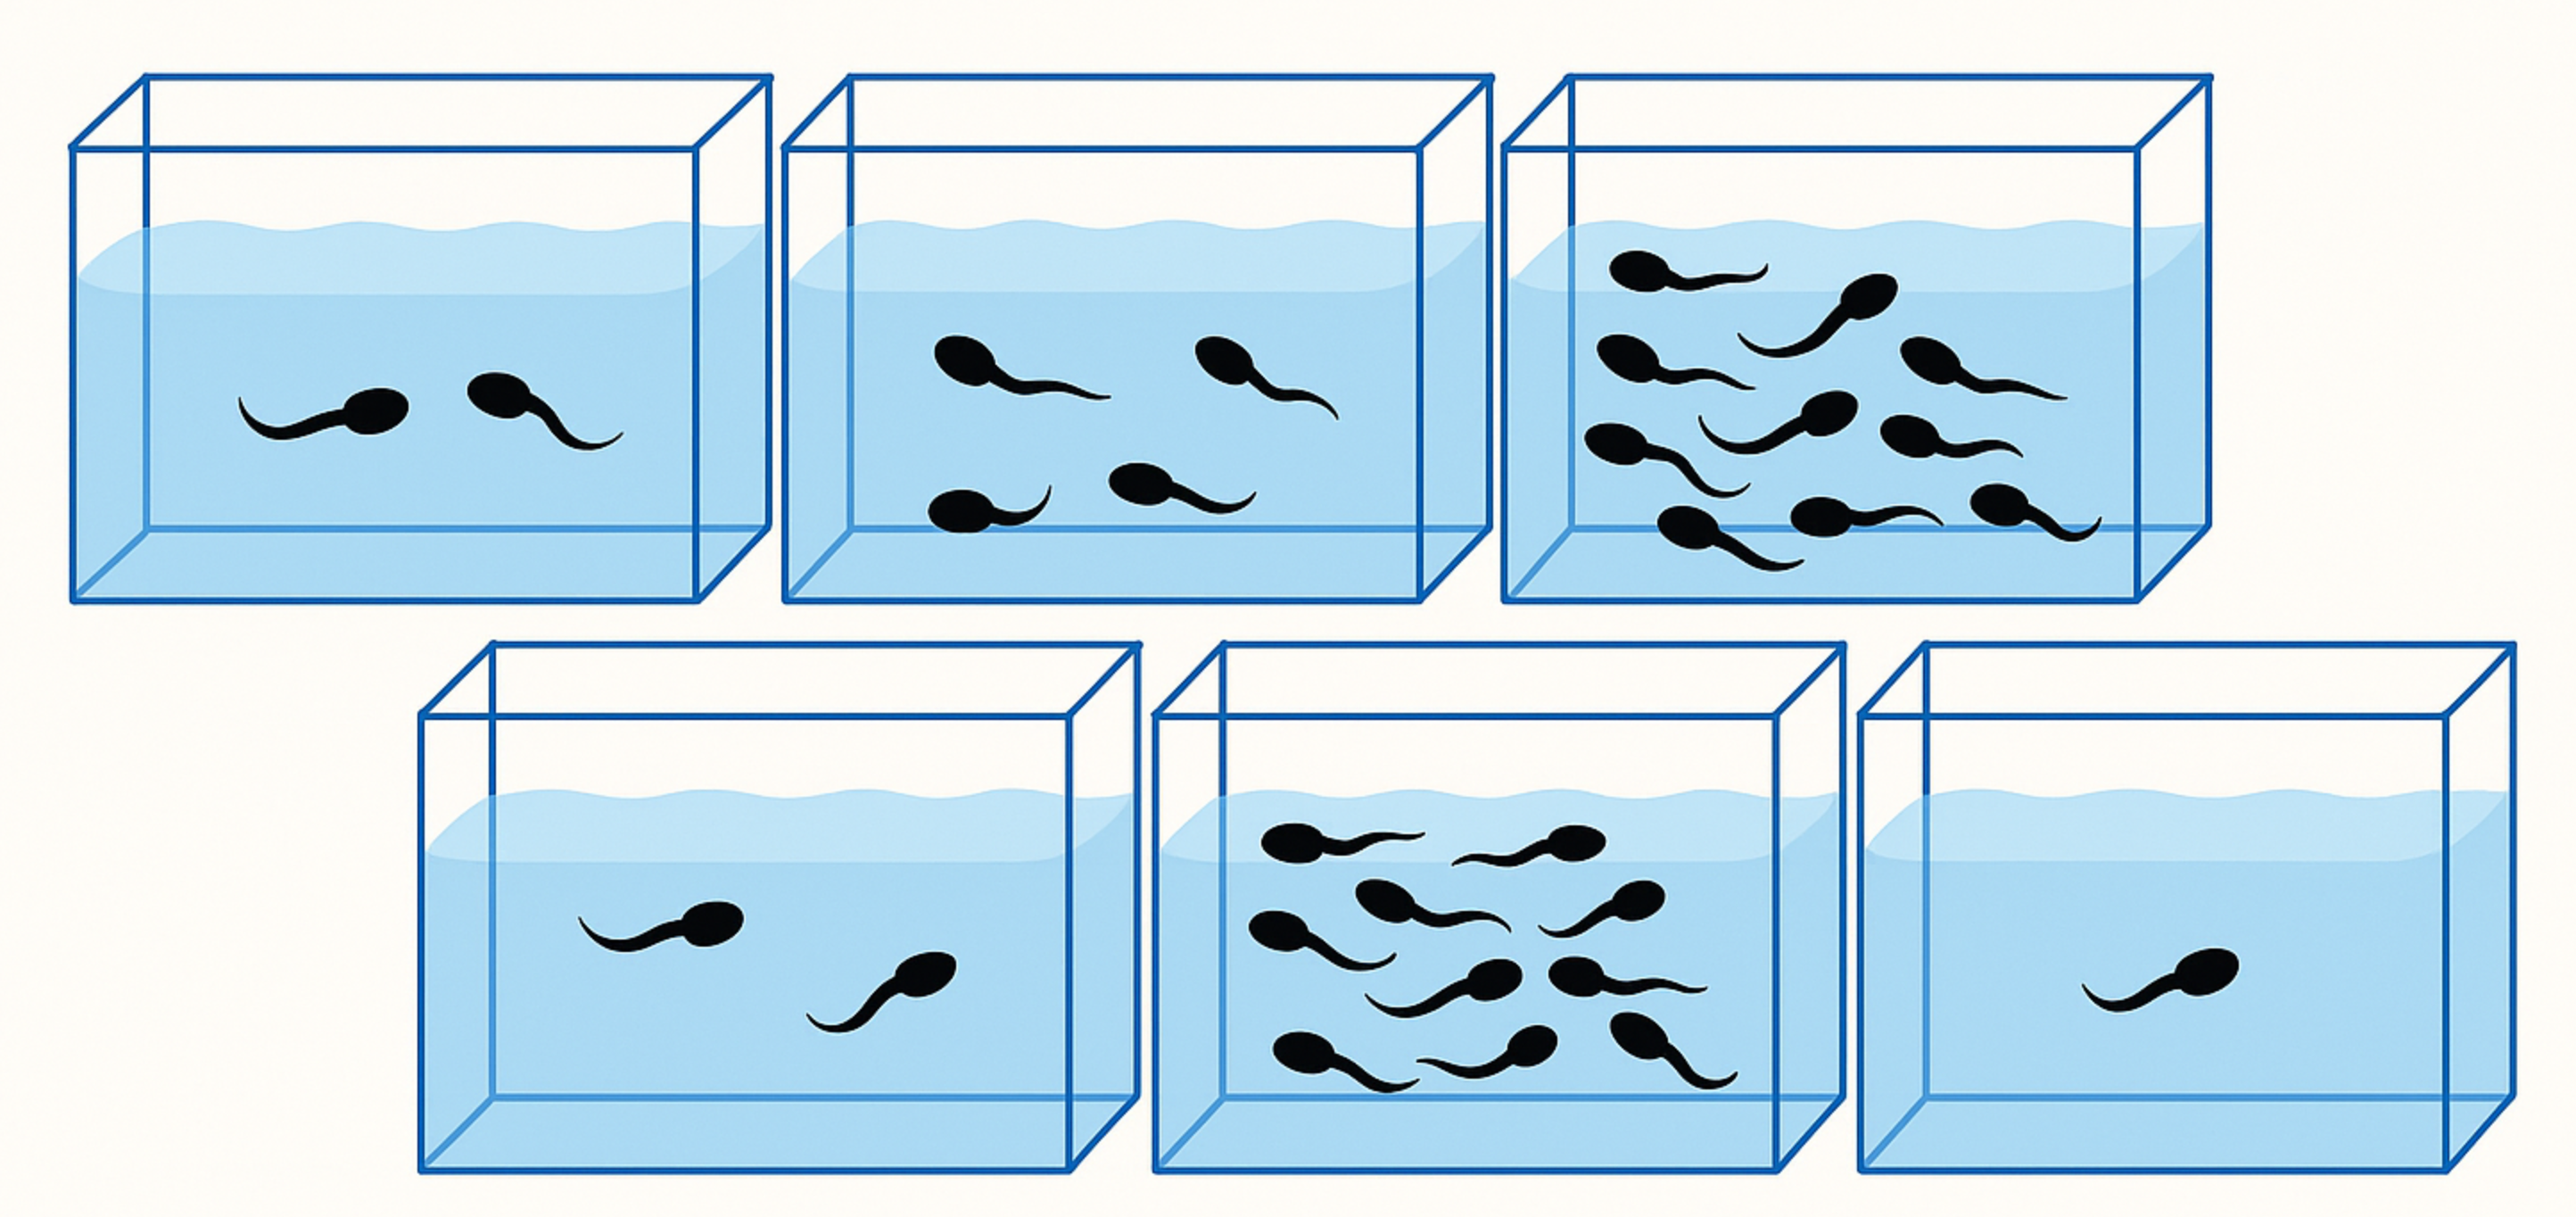
\includegraphics[keepaspectratio]{./images/tadpoles_in_tanks.png}}

\begin{Shaded}
\begin{Highlighting}[]
\FunctionTok{library}\NormalTok{(rethinking)}
\end{Highlighting}
\end{Shaded}

\begin{verbatim}
## Loading required package: cmdstanr
\end{verbatim}

\begin{verbatim}
## This is cmdstanr version 0.8.1.9000
\end{verbatim}

\begin{verbatim}
## - CmdStanR documentation and vignettes: mc-stan.org/cmdstanr
\end{verbatim}

\begin{verbatim}
## - CmdStan path: /Users/juergen/.cmdstan/cmdstan-2.36.0
\end{verbatim}

\begin{verbatim}
## - CmdStan version: 2.36.0
\end{verbatim}

\begin{verbatim}
## Loading required package: posterior
\end{verbatim}

\begin{verbatim}
## This is posterior version 1.6.1
\end{verbatim}

\begin{verbatim}
## 
## Attaching package: 'posterior'
\end{verbatim}

\begin{verbatim}
## The following objects are masked from 'package:stats':
## 
##     mad, sd, var
\end{verbatim}

\begin{verbatim}
## The following objects are masked from 'package:base':
## 
##     %in%, match
\end{verbatim}

\begin{verbatim}
## Loading required package: parallel
\end{verbatim}

\begin{verbatim}
## rethinking (Version 2.42)
\end{verbatim}

\begin{verbatim}
## 
## Attaching package: 'rethinking'
\end{verbatim}

\begin{verbatim}
## The following object is masked from 'package:stats':
## 
##     rstudent
\end{verbatim}

\begin{Shaded}
\begin{Highlighting}[]
\FunctionTok{library}\NormalTok{(lme4)}
\end{Highlighting}
\end{Shaded}

\begin{verbatim}
## Loading required package: Matrix
\end{verbatim}

\begin{Shaded}
\begin{Highlighting}[]
\FunctionTok{data}\NormalTok{(reedfrogs)}
\NormalTok{d }\OtherTok{\textless{}{-}}\NormalTok{ reedfrogs}
\FunctionTok{str}\NormalTok{(d)}
\end{Highlighting}
\end{Shaded}

\begin{verbatim}
## 'data.frame':    48 obs. of  5 variables:
##  $ density : int  10 10 10 10 10 10 10 10 10 10 ...
##  $ pred    : Factor w/ 2 levels "no","pred": 1 1 1 1 1 1 1 1 2 2 ...
##  $ size    : Factor w/ 2 levels "big","small": 1 1 1 1 2 2 2 2 1 1 ...
##  $ surv    : int  9 10 7 10 9 9 10 9 4 9 ...
##  $ propsurv: num  0.9 1 0.7 1 0.9 0.9 1 0.9 0.4 0.9 ...
\end{verbatim}

Variables are explained
\href{https://www.rdocumentation.org/packages/rethinking/versions/2.13/topics/reedfrogs}{here}
(see also p.401 in the book). The original paper can be found
\href{https://link.springer.com/article/10.1007/s00442-004-1806-x}{here}.

The number of surviving
\href{https://en.wikipedia.org/wiki/Tadpole}{tadpoles} \emph{surv}
should be modeled. Now, each row is a different ``tank'' (\(48\) in
total), an experimental environment that contains tadpoles. Obviously,
the tanks are one option for \emph{clustering} the data, assuming the
tadpoles within the same tank live in a more similar environment than
those in different tanks (or get a more similiar ``treatment''). We
could rewrite the data set to have one row per individual tadpole
(instead of number of survived a binary variable) and the cluster
variable called \emph{tank} (\hyperref[exercise1_LMM]{exercise 1}). We
would then model the survival probability of tadpoles (\(1\) could mean
\emph{survived} and \(0\) could mean \emph{died}). Formally, this would
be a so-called
\href{https://en.wikipedia.org/wiki/Logistic_regression}{logistic
regression} (see below), since our outcome is binary
(\emph{survided}/\emph{died}).

When estimating the number of surviving tadpoles we could consider the
following options:

\begin{itemize}
\tightlist
\item
  \textbf{Complete pooling} (\hyperref[exercise6_LMM]{exercise 6}):
  Estimate the overall survival probability (ignoring the tank effect).
  In this case, one might miss between-variance from the different
  tanks. A single intercept is used for all tanks.
\item
  \textbf{No pooling}: Estimate the survival probability for each tank
  (ignoring the overall effect completely). Here, the tanks do not
  ``know'' anything from one another. Information of one tank is not
  used for the other tanks. An intercept is estimated for each tank
  (\(48\) in total). This approach would be equivalent to using
  indicator variables for each tank.
\item
  \textbf{Partial pooling}: Estimate the survival probability for each
  tank, but use information from the other tanks.
\end{itemize}

\paragraph{Model 13.1. Partial pooling using regularizing
priors}\label{model13_1}

Let's start with the second model (intercept for each tank) with a
regularizing prior. We want to model the number of surviving tadpoles in
the tanks by using a binomial distribution with different survival
probabilities for each tank.

Here is our model in the typical notation:

\[
\begin{array}{rcl}
S_i &\sim& Binomial(N_i, p_i) \\
logit(p) &=& \alpha_{TANK}[i] \\
\alpha_j &\sim& \text{Normal}(0, 1.5)~\text{for } j=1,\ldots,48
\end{array}
\]

This is a \textbf{varying intercept model} (the simplest kind of
\textbf{varying effects} model) with \(48\) intercepts (one for each
tank).

The number of surviving tadpoles \(S_i\) in tank \(i\) is modeled as a
binomial distribution with \(N_i\) trials (the number of tadpoles in the
tank) and \(p_i\) the survival probability of tank \(i\). The
\textbf{regularizing priors} for \(\alpha_j\) is a normal distribution
with mean \(0\) and standard deviation \(1.5\).

Technically, \textbf{we could use different priors for each intercept},
but this would be a bit cumbersome and we do not have useful prior
information about the survival probabilities of the tanks.

Notice that we use a \texttt{logit} link function to transform the
probability \(p\) (range \((0,1)\)) to the range \((-\infty, \infty)\).
This way, we can use a normal distribution for the prior of the
intercepts. The inverse of the logit function is also available in
\texttt{rethinking}: \texttt{inv\_logit}.
\texttt{rethinking::inv\_logit(0)}gives the probability of \(0.5\). So,
we assume a coin flip for the survival probability of the tadpoles in
the tanks \emph{a priori} (maybe not the worst starting point if you
have no clue).

What survaival probabilities do we assume a priori? Well, according to
the normal distribution with a standard deviation of \(1.5\) we assume
that the 95\% of the logit-transformed survival probabilities are
between \(-3\) and \(3\). This means that the survival probabilities in
the tanks are in:

\begin{Shaded}
\begin{Highlighting}[]
\FunctionTok{c}\NormalTok{(rethinking}\SpecialCharTok{::}\FunctionTok{inv\_logit}\NormalTok{(}\SpecialCharTok{{-}}\DecValTok{3}\NormalTok{), rethinking}\SpecialCharTok{::}\FunctionTok{inv\_logit}\NormalTok{(}\DecValTok{3}\NormalTok{))}
\end{Highlighting}
\end{Shaded}

\begin{verbatim}
## [1] 0.04742587 0.95257413
\end{verbatim}

This assumption seems rather reasonable and survival probabilities are
not constrained very much.

Next we define the data set for the model and use the \texttt{ulam}
function from the \texttt{rethinking} package to fit the model.

\begin{Shaded}
\begin{Highlighting}[]
\FunctionTok{library}\NormalTok{(rethinking)}

\NormalTok{d}\SpecialCharTok{$}\NormalTok{tank }\OtherTok{\textless{}{-}} \DecValTok{1}\SpecialCharTok{:}\FunctionTok{nrow}\NormalTok{(d)}
\NormalTok{dat }\OtherTok{\textless{}{-}} \FunctionTok{list}\NormalTok{(}\AttributeTok{S =}\NormalTok{ d}\SpecialCharTok{$}\NormalTok{surv,}
            \AttributeTok{N =}\NormalTok{ d}\SpecialCharTok{$}\NormalTok{density,}
            \AttributeTok{tank =}\NormalTok{ d}\SpecialCharTok{$}\NormalTok{tank)}

\CommentTok{\# approximate posterior}
\FunctionTok{set.seed}\NormalTok{(}\DecValTok{122}\NormalTok{)}
\NormalTok{m13}\FloatTok{.1} \OtherTok{\textless{}{-}} \FunctionTok{ulam}\NormalTok{(}
  \FunctionTok{alist}\NormalTok{(}
\NormalTok{    S }\SpecialCharTok{\textasciitilde{}} \FunctionTok{dbinom}\NormalTok{(N, p),}
    \FunctionTok{logit}\NormalTok{(p) }\OtherTok{\textless{}{-}}\NormalTok{ a[tank],}
\NormalTok{    a[tank] }\SpecialCharTok{\textasciitilde{}} \FunctionTok{dnorm}\NormalTok{(}\DecValTok{0}\NormalTok{, }\FloatTok{1.5}\NormalTok{)}
\NormalTok{  ) , }\AttributeTok{data =}\NormalTok{ dat, }
  \AttributeTok{chains =} \DecValTok{4}\NormalTok{, }
  \AttributeTok{log\_lik =} \ConstantTok{TRUE}\NormalTok{,}
  \AttributeTok{cores =} \FunctionTok{detectCores}\NormalTok{() }\SpecialCharTok{{-}} \DecValTok{1}\NormalTok{)}
\end{Highlighting}
\end{Shaded}

\begin{verbatim}
## Running MCMC with 4 chains, at most 7 in parallel, with 1 thread(s) per chain...
## 
## Chain 1 Iteration:   1 / 1000 [  0%]  (Warmup) 
## Chain 1 Iteration: 100 / 1000 [ 10%]  (Warmup) 
## Chain 1 Iteration: 200 / 1000 [ 20%]  (Warmup) 
## Chain 1 Iteration: 300 / 1000 [ 30%]  (Warmup) 
## Chain 1 Iteration: 400 / 1000 [ 40%]  (Warmup) 
## Chain 1 Iteration: 500 / 1000 [ 50%]  (Warmup) 
## Chain 1 Iteration: 501 / 1000 [ 50%]  (Sampling) 
## Chain 1 Iteration: 600 / 1000 [ 60%]  (Sampling) 
## Chain 1 Iteration: 700 / 1000 [ 70%]  (Sampling) 
## Chain 1 Iteration: 800 / 1000 [ 80%]  (Sampling) 
## Chain 1 Iteration: 900 / 1000 [ 90%]  (Sampling) 
## Chain 1 Iteration: 1000 / 1000 [100%]  (Sampling) 
## Chain 2 Iteration:   1 / 1000 [  0%]  (Warmup) 
## Chain 2 Iteration: 100 / 1000 [ 10%]  (Warmup) 
## Chain 2 Iteration: 200 / 1000 [ 20%]  (Warmup) 
## Chain 2 Iteration: 300 / 1000 [ 30%]  (Warmup) 
## Chain 2 Iteration: 400 / 1000 [ 40%]  (Warmup) 
## Chain 2 Iteration: 500 / 1000 [ 50%]  (Warmup) 
## Chain 2 Iteration: 501 / 1000 [ 50%]  (Sampling) 
## Chain 2 Iteration: 600 / 1000 [ 60%]  (Sampling) 
## Chain 2 Iteration: 700 / 1000 [ 70%]  (Sampling) 
## Chain 2 Iteration: 800 / 1000 [ 80%]  (Sampling) 
## Chain 2 Iteration: 900 / 1000 [ 90%]  (Sampling) 
## Chain 2 Iteration: 1000 / 1000 [100%]  (Sampling) 
## Chain 3 Iteration:   1 / 1000 [  0%]  (Warmup) 
## Chain 3 Iteration: 100 / 1000 [ 10%]  (Warmup) 
## Chain 3 Iteration: 200 / 1000 [ 20%]  (Warmup) 
## Chain 3 Iteration: 300 / 1000 [ 30%]  (Warmup) 
## Chain 3 Iteration: 400 / 1000 [ 40%]  (Warmup) 
## Chain 3 Iteration: 500 / 1000 [ 50%]  (Warmup) 
## Chain 3 Iteration: 501 / 1000 [ 50%]  (Sampling) 
## Chain 3 Iteration: 600 / 1000 [ 60%]  (Sampling) 
## Chain 3 Iteration: 700 / 1000 [ 70%]  (Sampling) 
## Chain 3 Iteration: 800 / 1000 [ 80%]  (Sampling) 
## Chain 3 Iteration: 900 / 1000 [ 90%]  (Sampling) 
## Chain 3 Iteration: 1000 / 1000 [100%]  (Sampling) 
## Chain 4 Iteration:   1 / 1000 [  0%]  (Warmup) 
## Chain 4 Iteration: 100 / 1000 [ 10%]  (Warmup) 
## Chain 4 Iteration: 200 / 1000 [ 20%]  (Warmup) 
## Chain 4 Iteration: 300 / 1000 [ 30%]  (Warmup) 
## Chain 4 Iteration: 400 / 1000 [ 40%]  (Warmup) 
## Chain 4 Iteration: 500 / 1000 [ 50%]  (Warmup) 
## Chain 4 Iteration: 501 / 1000 [ 50%]  (Sampling) 
## Chain 4 Iteration: 600 / 1000 [ 60%]  (Sampling) 
## Chain 4 Iteration: 700 / 1000 [ 70%]  (Sampling) 
## Chain 4 Iteration: 800 / 1000 [ 80%]  (Sampling) 
## Chain 4 Iteration: 900 / 1000 [ 90%]  (Sampling) 
## Chain 4 Iteration: 1000 / 1000 [100%]  (Sampling) 
## Chain 1 finished in 0.1 seconds.
## Chain 2 finished in 0.1 seconds.
## Chain 3 finished in 0.1 seconds.
## Chain 4 finished in 0.1 seconds.
## 
## All 4 chains finished successfully.
## Mean chain execution time: 0.1 seconds.
## Total execution time: 0.2 seconds.
\end{verbatim}

\begin{Shaded}
\begin{Highlighting}[]
\FunctionTok{precis}\NormalTok{(m13}\FloatTok{.1}\NormalTok{, }\AttributeTok{depth =} \DecValTok{2}\NormalTok{)}
\end{Highlighting}
\end{Shaded}

\begin{verbatim}
##               mean        sd        5.5%       94.5%      rhat ess_bulk
## a[1]   1.717154006 0.7747045  0.54616751  3.00284170 1.0000687 3842.501
## a[2]   2.428617822 0.9211741  1.06824055  4.00015385 1.0012690 3260.212
## a[3]   0.752957586 0.6606081 -0.30096467  1.87725390 0.9994289 3657.926
## a[4]   2.392671596 0.9029471  1.04232310  3.96444320 0.9999341 4901.360
## a[5]   1.698600986 0.7501296  0.56599784  2.95760400 1.0010747 3583.085
## a[6]   1.709016626 0.7333373  0.61628599  2.93631575 1.0043948 3791.625
## a[7]   2.394662704 0.8967971  1.05357265  3.91037710 1.0021691 4633.411
## a[8]   1.751520527 0.8358778  0.51949731  3.11502600 1.0010314 2908.886
## a[9]  -0.368916633 0.6263820 -1.40362045  0.63108741 1.0014184 5011.742
## a[10]  1.721989971 0.7876527  0.53971156  3.01818445 1.0064067 4743.990
## a[11]  0.762625202 0.6504815 -0.23379561  1.84594325 1.0042895 4356.338
## a[12]  0.360839662 0.6212530 -0.61653294  1.35696620 1.0003393 5427.338
## a[13]  0.747187659 0.6556836 -0.26629876  1.86578240 1.0047650 4965.966
## a[14]  0.004006226 0.6030814 -0.96596033  0.95626616 1.0015451 3860.382
## a[15]  1.698071502 0.7557423  0.58532612  3.00604665 1.0044770 4060.982
## a[16]  1.718281276 0.7589570  0.55788234  3.01417210 0.9995458 4085.653
## a[17]  2.540229640 0.6715384  1.51315760  3.67929090 1.0045229 3551.210
## a[18]  2.143608256 0.6099572  1.24664285  3.19176460 1.0027772 4601.028
## a[19]  1.814013282 0.5661173  0.96992496  2.74369310 1.0008102 3875.396
## a[20]  3.123650833 0.8415721  1.90725255  4.55287270 1.0001108 4325.296
## a[21]  2.144628056 0.6206063  1.21321885  3.18875240 1.0003712 4533.942
## a[22]  2.147574902 0.5862451  1.27518855  3.13301315 1.0054417 3115.241
## a[23]  2.158113205 0.6232680  1.23542735  3.20262840 1.0031826 4470.846
## a[24]  1.559385117 0.5054760  0.81471935  2.39450025 1.0050444 4677.140
## a[25] -1.100464102 0.4645629 -1.90970175 -0.37079074 1.0031187 4404.834
## a[26]  0.066658204 0.3997793 -0.57122361  0.71319580 1.0064293 5082.203
## a[27] -1.543870059 0.4969425 -2.35267600 -0.80927273 1.0049318 4888.677
## a[28] -0.545686639 0.3798291 -1.16412750  0.05957414 1.0141192 4539.855
## a[29]  0.076432999 0.3891808 -0.54687735  0.68588656 1.0063621 4372.045
## a[30]  1.317149701 0.4699257  0.61627877  2.10864310 1.0045814 4237.156
## a[31] -0.730232329 0.4142389 -1.41215210 -0.08699833 1.0056791 4674.458
## a[32] -0.380477602 0.3973004 -1.02838145  0.22966973 1.0027171 4757.953
## a[33]  2.854476850 0.6688006  1.86231770  3.93923980 1.0028748 4265.441
## a[34]  2.465178502 0.6016136  1.57307340  3.49223990 1.0034665 4026.537
## a[35]  2.475988085 0.6001981  1.62509180  3.45605210 1.0022452 3520.649
## a[36]  1.906146592 0.4793998  1.17540695  2.69468780 1.0091406 3637.720
## a[37]  1.903268812 0.4848702  1.17045730  2.68925485 0.9999314 4580.692
## a[38]  3.377291100 0.7728682  2.21480150  4.70722490 0.9999677 3559.742
## a[39]  2.448119286 0.5794139  1.58287005  3.42906255 1.0005167 4544.304
## a[40]  2.154826607 0.5110004  1.38358250  3.05123950 1.0057481 3928.734
## a[41] -1.924960111 0.4805039 -2.72391445 -1.20680920 1.0003669 3217.189
## a[42] -0.639489130 0.3594361 -1.20374385 -0.07755664 1.0036102 3891.702
## a[43] -0.515434665 0.3438150 -1.06684055  0.01709138 1.0067069 3206.309
## a[44] -0.399514162 0.3554107 -0.97334898  0.16487656 1.0043647 5212.318
## a[45]  0.519393681 0.3592609 -0.05772033  1.08264245 1.0022088 4807.785
## a[46] -0.636130179 0.3468987 -1.20742535 -0.10853365 1.0071298 3963.335
## a[47]  1.919195782 0.4916630  1.16999095  2.74101715 1.0000987 3428.411
## a[48] -0.061061407 0.3286406 -0.57313044  0.45005764 1.0009603 3435.612
\end{verbatim}

\begin{Shaded}
\begin{Highlighting}[]
\CommentTok{\# expected survival in tank 1}
\NormalTok{rethinking}\SpecialCharTok{::}\FunctionTok{logistic}\NormalTok{(}\FloatTok{1.717154006}\NormalTok{) }\CommentTok{\# same as inv\_logit(1.717154006)}
\end{Highlighting}
\end{Shaded}

\begin{verbatim}
## [1] 0.8477619
\end{verbatim}

The R-output from \texttt{precis(m13.1,\ depth\ =\ 2)}shows the
posterior means and standard deviations of our \(48\) intercepts (\(48\)
tanks with tadpoles). These intercepts are on the scale
\((-\infty, \infty)\).

Note that you can always switch from the range \((-\infty, \infty)\) to
a probability using the \texttt{logistic} function from the
\texttt{rethinking} package - these functions are called \emph{squashing
functions} for a reason. The \texttt{inv\_logit}function does the same.

\[
\mathrm{logistic}(x) = \mathrm{inv\_logit}(x) = \frac{1}{1 + e^{-x}}
\]

The other way around works as well, using the \texttt{logit} function.
\[\text{logit}(p) = \log\left( \frac{p}{1 - p} \right)\]

Let's quickly see if these are indeed inverse functions of each other
-\textgreater{} \hyperref[exercise5_LMM]{exercise 5}.

\paragraph{Model 13.2: Partial pooling using adaptive
pooling}\label{model13_2}

\textbf{Next}, we use \textbf{adaptive pooling}. For this, we use priors
for the \texttt{a{[}tank{]}} parameters, but know they \emph{know} from
each other via the prior for \(\bar{\alpha}\). This model learns from
the data how much the intercepts should be pulled towards a common mean.
Now we have an additional level in the model hierarchy:

\begin{itemize}
\tightlist
\item
  In the \textbf{top level}, the outcome is \(S\), the parameters are
  the intercepts \(\alpha_{TANK[i]}\), and the priors are
  \(\alpha_j \sim N(\bar{\alpha}, \sigma)\).
\item
  In the \textbf{second level}, the ``outcome'' are the intercepts
  \(\alpha_{TANK[i]}\), the parameters are \(\bar{\alpha}\) and
  \(\sigma\), and the priors are \(\bar{\alpha} \sim N(0, 1.5)\) and
  \(\sigma \sim \text{Exponential}(1)\).
\end{itemize}

\[
\begin{array}{rcl}
S_i &\sim& \text{Binomial}(N_i, p_i) \\
\text{logit}(p) &=& \alpha_{\text{TANK}[i]} \\
\alpha_j &\sim& \text{Normal}(\bar{\alpha}, \sigma)\\
\bar{\alpha} &\sim& \text{Normal}(0, 1.5)\\
\sigma &\sim& \text{Exponential}(1)
\end{array}
\]

Since the parameters in the prior of the \(\alpha_j\) have also priors
(last two lines are new), we have a \emph{multilevel} model. In this
case, we have \emph{two} levels and the parameters \(\bar{\alpha}\) and
\(\sigma\) are called \textbf{hyperparameters}. The priors of the
hyperparameters are called \textbf{hyperpriors}. The \textbf{amount or
regularization is controlled by the hyperparameter} \(\sigma\) and is
learned from the data. \(\sigma\) controls, how much the intercepts are
allowed to deviate from the mean \(\bar{\alpha}\). The smaller
\(\sigma\), the more the intercepts are pulled towards the mean
\(\bar{\alpha}\).

Below, we see the model hierarchy:

\pandocbounded{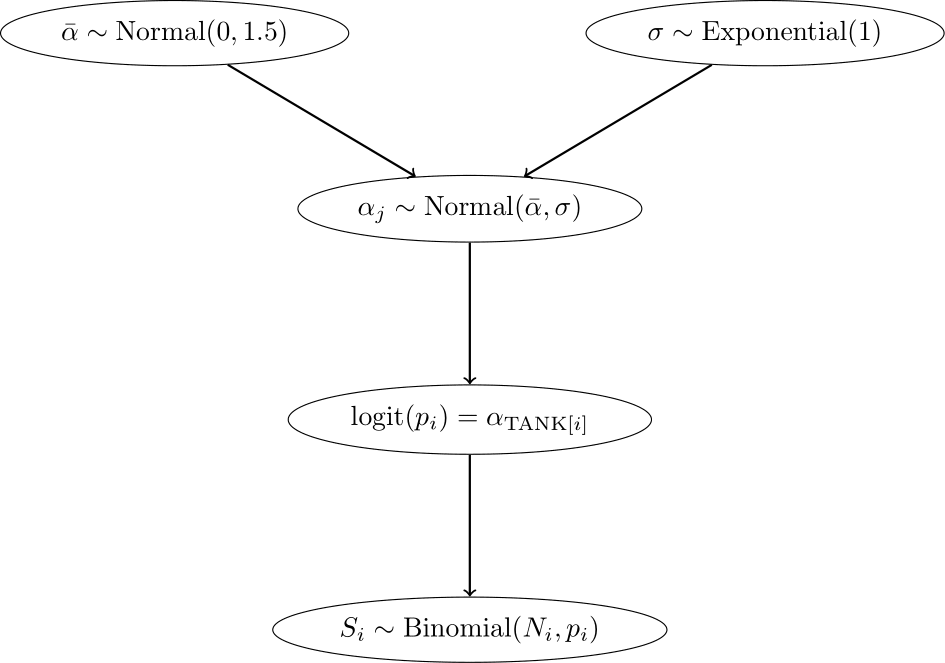
\includegraphics[keepaspectratio]{./images/Model_Hier_LMM_1.png}}

We now fit the model using the \texttt{ulam} function from the
\texttt{rethinking} package.

\begin{Shaded}
\begin{Highlighting}[]
\FunctionTok{library}\NormalTok{(conflicted)}
\FunctionTok{conflicts\_prefer}\NormalTok{(posterior}\SpecialCharTok{::}\NormalTok{var)}
\end{Highlighting}
\end{Shaded}

\begin{verbatim}
## [conflicted] Will prefer posterior::var over any other package.
\end{verbatim}

\begin{Shaded}
\begin{Highlighting}[]
\FunctionTok{conflicts\_prefer}\NormalTok{(posterior}\SpecialCharTok{::}\NormalTok{sd)}
\end{Highlighting}
\end{Shaded}

\begin{verbatim}
## [conflicted] Will prefer posterior::sd over any other package.
\end{verbatim}

\begin{Shaded}
\begin{Highlighting}[]
\NormalTok{m13}\FloatTok{.2} \OtherTok{\textless{}{-}} \FunctionTok{ulam}\NormalTok{(}
  \FunctionTok{alist}\NormalTok{(}
\NormalTok{    S }\SpecialCharTok{\textasciitilde{}} \FunctionTok{dbinom}\NormalTok{(N, p),}
    \FunctionTok{logit}\NormalTok{(p) }\OtherTok{\textless{}{-}}\NormalTok{ a[tank],}
\NormalTok{    a[tank] }\SpecialCharTok{\textasciitilde{}} \FunctionTok{dnorm}\NormalTok{(a\_bar, sigma),}
\NormalTok{    a\_bar }\SpecialCharTok{\textasciitilde{}} \FunctionTok{dnorm}\NormalTok{(}\DecValTok{0}\NormalTok{, }\FloatTok{1.5}\NormalTok{),}
\NormalTok{    sigma }\SpecialCharTok{\textasciitilde{}} \FunctionTok{dexp}\NormalTok{(}\DecValTok{1}\NormalTok{)}
\NormalTok{  ) , }\AttributeTok{data =}\NormalTok{ dat, }
  \AttributeTok{chains =} \DecValTok{4}\NormalTok{, }
  \AttributeTok{log\_lik =} \ConstantTok{TRUE}\NormalTok{,}
  \AttributeTok{cores =} \FunctionTok{detectCores}\NormalTok{() }\SpecialCharTok{{-}} \DecValTok{1}\NormalTok{)}
\end{Highlighting}
\end{Shaded}

\begin{verbatim}
## Running MCMC with 4 chains, at most 7 in parallel, with 1 thread(s) per chain...
## 
## Chain 1 Iteration:   1 / 1000 [  0%]  (Warmup) 
## Chain 1 Iteration: 100 / 1000 [ 10%]  (Warmup) 
## Chain 1 Iteration: 200 / 1000 [ 20%]  (Warmup) 
## Chain 1 Iteration: 300 / 1000 [ 30%]  (Warmup) 
## Chain 1 Iteration: 400 / 1000 [ 40%]  (Warmup) 
## Chain 1 Iteration: 500 / 1000 [ 50%]  (Warmup) 
## Chain 1 Iteration: 501 / 1000 [ 50%]  (Sampling) 
## Chain 1 Iteration: 600 / 1000 [ 60%]  (Sampling) 
## Chain 1 Iteration: 700 / 1000 [ 70%]  (Sampling) 
## Chain 1 Iteration: 800 / 1000 [ 80%]  (Sampling) 
## Chain 1 Iteration: 900 / 1000 [ 90%]  (Sampling) 
## Chain 1 Iteration: 1000 / 1000 [100%]  (Sampling) 
## Chain 2 Iteration:   1 / 1000 [  0%]  (Warmup) 
## Chain 2 Iteration: 100 / 1000 [ 10%]  (Warmup) 
## Chain 2 Iteration: 200 / 1000 [ 20%]  (Warmup) 
## Chain 2 Iteration: 300 / 1000 [ 30%]  (Warmup) 
## Chain 2 Iteration: 400 / 1000 [ 40%]  (Warmup) 
## Chain 2 Iteration: 500 / 1000 [ 50%]  (Warmup) 
## Chain 2 Iteration: 501 / 1000 [ 50%]  (Sampling) 
## Chain 2 Iteration: 600 / 1000 [ 60%]  (Sampling) 
## Chain 2 Iteration: 700 / 1000 [ 70%]  (Sampling) 
## Chain 2 Iteration: 800 / 1000 [ 80%]  (Sampling) 
## Chain 2 Iteration: 900 / 1000 [ 90%]  (Sampling) 
## Chain 2 Iteration: 1000 / 1000 [100%]  (Sampling) 
## Chain 3 Iteration:   1 / 1000 [  0%]  (Warmup) 
## Chain 3 Iteration: 100 / 1000 [ 10%]  (Warmup) 
## Chain 3 Iteration: 200 / 1000 [ 20%]  (Warmup) 
## Chain 3 Iteration: 300 / 1000 [ 30%]  (Warmup) 
## Chain 3 Iteration: 400 / 1000 [ 40%]  (Warmup) 
## Chain 3 Iteration: 500 / 1000 [ 50%]  (Warmup) 
## Chain 3 Iteration: 501 / 1000 [ 50%]  (Sampling) 
## Chain 3 Iteration: 600 / 1000 [ 60%]  (Sampling) 
## Chain 3 Iteration: 700 / 1000 [ 70%]  (Sampling) 
## Chain 3 Iteration: 800 / 1000 [ 80%]  (Sampling) 
## Chain 3 Iteration: 900 / 1000 [ 90%]  (Sampling) 
## Chain 3 Iteration: 1000 / 1000 [100%]  (Sampling) 
## Chain 4 Iteration:   1 / 1000 [  0%]  (Warmup) 
## Chain 4 Iteration: 100 / 1000 [ 10%]  (Warmup) 
## Chain 4 Iteration: 200 / 1000 [ 20%]  (Warmup) 
## Chain 4 Iteration: 300 / 1000 [ 30%]  (Warmup) 
## Chain 4 Iteration: 400 / 1000 [ 40%]  (Warmup) 
## Chain 4 Iteration: 500 / 1000 [ 50%]  (Warmup) 
## Chain 4 Iteration: 501 / 1000 [ 50%]  (Sampling) 
## Chain 4 Iteration: 600 / 1000 [ 60%]  (Sampling) 
## Chain 4 Iteration: 700 / 1000 [ 70%]  (Sampling) 
## Chain 4 Iteration: 800 / 1000 [ 80%]  (Sampling) 
## Chain 4 Iteration: 900 / 1000 [ 90%]  (Sampling) 
## Chain 4 Iteration: 1000 / 1000 [100%]  (Sampling)
\end{verbatim}

\begin{verbatim}
## Chain 4 Informational Message: The current Metropolis proposal is about to be rejected because of the following issue:
## Chain 4 Exception: normal_lpdf: Scale parameter is 0, but must be positive! (in '/var/folders/pm/jd6n6gj10371_bml1gh8sc5w0000gn/T/RtmpMWR7Ha/model-183252f18a621.stan', line 15, column 4 to column 32)
## Chain 4 If this warning occurs sporadically, such as for highly constrained variable types like covariance matrices, then the sampler is fine,
## Chain 4 but if this warning occurs often then your model may be either severely ill-conditioned or misspecified.
## Chain 4
\end{verbatim}

\begin{verbatim}
## Chain 1 finished in 0.1 seconds.
## Chain 2 finished in 0.1 seconds.
## Chain 3 finished in 0.1 seconds.
## Chain 4 finished in 0.1 seconds.
## 
## All 4 chains finished successfully.
## Mean chain execution time: 0.1 seconds.
## Total execution time: 0.2 seconds.
\end{verbatim}

\begin{Shaded}
\begin{Highlighting}[]
\FunctionTok{precis}\NormalTok{(m13}\FloatTok{.2}\NormalTok{, }\AttributeTok{depth =} \DecValTok{2}\NormalTok{)}
\end{Highlighting}
\end{Shaded}

\begin{verbatim}
##                mean        sd        5.5%        94.5%      rhat ess_bulk
## a[1]   2.1360104954 0.8661191  0.83424198  3.553682700 1.0026805 3270.394
## a[2]   3.0781335085 1.1236851  1.43096300  4.984337950 1.0021514 3333.772
## a[3]   1.0172166998 0.6728834  0.02487391  2.122557100 1.0017997 4433.035
## a[4]   3.0539084560 1.0673010  1.45577985  4.862345550 0.9991935 3292.307
## a[5]   2.1460704153 0.8885053  0.82128835  3.632871100 1.0012996 3243.212
## a[6]   2.1295681940 0.8491091  0.88580128  3.547453050 1.0068927 4014.260
## a[7]   3.0995747675 1.1423048  1.49656170  5.081114500 1.0000324 2876.988
## a[8]   2.1399446424 0.9003458  0.81845163  3.682066500 1.0014370 3989.652
## a[9]  -0.1714730123 0.6191399 -1.18887420  0.817493905 1.0011313 3485.167
## a[10]  2.0975422705 0.8315647  0.86475233  3.491159800 1.0003507 3475.655
## a[11]  0.9972846111 0.6886670 -0.06780398  2.108900800 1.0035689 6346.111
## a[12]  0.5808274429 0.6321307 -0.39005998  1.589965800 1.0073548 4009.231
## a[13]  1.0044482950 0.6869233 -0.06659326  2.145820400 1.0062364 5228.172
## a[14]  0.1943572393 0.5958137 -0.75088828  1.137035850 1.0090229 4741.338
## a[15]  2.1509188614 0.8679934  0.90383891  3.653387850 1.0031940 3312.879
## a[16]  2.1333640552 0.9017144  0.80812878  3.653567300 1.0126010 4233.256
## a[17]  2.9192000930 0.8415071  1.68621300  4.328422500 1.0040634 4410.077
## a[18]  2.3925664980 0.6551941  1.42167145  3.513079150 1.0056149 4144.799
## a[19]  2.0077513930 0.5900888  1.11100110  2.993477400 1.0059627 3633.662
## a[20]  3.6725677750 1.0278681  2.20375370  5.475839300 1.0049323 3236.751
## a[21]  2.4059350610 0.6759614  1.38493480  3.559096600 1.0015502 5132.563
## a[22]  2.4065305525 0.6796675  1.42094305  3.541692650 0.9991290 3831.139
## a[23]  2.3861532095 0.6514720  1.42360935  3.472103550 1.0043729 4128.680
## a[24]  1.7089185740 0.5393019  0.87925440  2.627249950 1.0048578 4608.699
## a[25] -1.0120972883 0.4472418 -1.73198540 -0.326257340 1.0014661 4734.657
## a[26]  0.1608543317 0.3886832 -0.46547174  0.767354565 1.0023246 4941.014
## a[27] -1.4196695957 0.4932724 -2.25709745 -0.685836175 1.0028562 4123.586
## a[28] -0.4766474294 0.4060361 -1.14774660  0.151370735 1.0052220 3931.755
## a[29]  0.1694769825 0.4170077 -0.49255198  0.859140040 1.0020527 4739.882
## a[30]  1.4511140548 0.5133738  0.66183801  2.306309700 1.0011993 4978.641
## a[31] -0.6385969972 0.4191422 -1.30238420  0.002327188 1.0021641 4600.143
## a[32] -0.3101703440 0.3728743 -0.90309567  0.287795040 0.9998292 5387.376
## a[33]  3.1774488200 0.7655335  2.08349505  4.549344000 1.0049724 3861.331
## a[34]  2.7053424900 0.6559522  1.73698945  3.801545200 1.0012059 4418.032
## a[35]  2.7221132200 0.6273888  1.81337830  3.780182650 1.0009124 3645.004
## a[36]  2.0546272795 0.4965714  1.31339900  2.878739800 1.0062188 4941.400
## a[37]  2.0584841305 0.5188968  1.26758275  2.917035500 1.0015659 4474.923
## a[38]  3.8972652500 0.9072140  2.63982515  5.508591850 1.0012459 3004.701
## a[39]  2.6974989445 0.6268090  1.74492005  3.751004950 0.9991983 3801.943
## a[40]  2.3462939655 0.5804959  1.47061030  3.318163350 1.0087612 3756.208
## a[41] -1.8135897265 0.4813845 -2.60774680 -1.085182300 1.0000863 3538.261
## a[42] -0.5797062286 0.3540843 -1.15873190 -0.026373790 1.0025961 3932.502
## a[43] -0.4553320681 0.3423639 -1.00197960  0.080289540 1.0064972 4788.740
## a[44] -0.3294683952 0.3311178 -0.86400261  0.191963110 1.0099484 4098.959
## a[45]  0.5781168532 0.3537311  0.02023151  1.152294850 1.0051871 4534.473
## a[46] -0.5734202532 0.3340746 -1.11167870 -0.052582168 1.0045535 3855.996
## a[47]  2.0729423255 0.5180042  1.30783735  2.935491000 1.0033394 3591.954
## a[48] -0.0003544386 0.3378852 -0.52970810  0.533022400 1.0060391 4423.905
## a_bar  1.3420237045 0.2527708  0.94567161  1.760416550 1.0011880 2994.562
## sigma  1.6149891850 0.2052025  1.30750950  1.961327050 0.9998544 1674.452
\end{verbatim}

Now, the output of \texttt{precis(m13.2,\ depth\ =\ 2)} additionally
shows the posterior means and standard deviations of the hyperparameters
\(\bar{\alpha}\) (\texttt{a\_bar}) and \(\sigma\) (\texttt{sigma}).

\paragraph{Conceptual difference between model 13.1 and
13.2}\label{conceptual-difference-between-model-13.1-and-13.2}

\textbf{Model 13.1} is not a multilevel model, we just tell the model
there are \(48\) tanks and each tank has its own intercept. For each
intercept, we use the same prior distribution (\(Normal (0, 1.5)\)), but
we could use different ones if we had knowledge about the survival
probabilities of some of the tanks. Note that the priors themselves are
not connected via another level. They do their thing independently.

\begin{itemize}
\item
  By \emph{decreasing} the variance of these priors, we are dampening
  the influence of the data on the intercepts which are drawn towards to
  overall mean.
\item
  \emph{Increasing} the variance of the priors to a value large enough
  will result in the raw survival probabilities for each tank. This
  would be the same as if we took indicator variables for each tank. See
  \hyperref[exercise2_LMM]{exercise 2}.
\end{itemize}

\textbf{Model 13.2} is a \textbf{multilevel model}. Now the model
\emph{learns from the data} from which overall mean and variance the
intercepts are drawn (\(Normal(\bar{\alpha}, \sigma)\)). The prior for
\(\bar{\alpha}\) expresses our belief about the mean survival
probability, while the prior for \(\sigma\) expresses our belief about
the variability of the survival probabilities.

\textbf{Figure 13.1 from the book} depicts the pooling effect of model
13.2. with respect to tadpole tank size.

\pandocbounded{
\includegraphics[keepaspectratio]{02-Further_Regression_Methods_files/figure-latex/unnamed-chunk-5-1.pdf}}

In \hyperref[exercise2_LMM]{exercise 2} we make the difference between
the models 13.1 and 2 clearer. Figure 13.1 from the book shows the
posterior survival probabilities for each tank from model 13.2 (black
circles) and raw survival probabilities (blue filled points). What we
can see is that the estimated survival probabilities for the
hierarchical model are drawn towards the mean overall survival
probability across all tanks (dashed line;
\(logistic(\bar{\alpha}) \approx 0.79\)).

\begin{itemize}
\tightlist
\item
  In large tanks, there is less shrinkage (enough
  information/observations), while in small tanks the estimates are
  pulled more towards the mean (information is used from other tanks).
\item
  The more extreme the raw survival probability (with respect to the
  overall survival probability), the more it is pulled towards the mean.
\end{itemize}

This is the \textbf{pooling} effect of the model. The phenomenon is
called \textbf{shrinkage}.

See also \hyperref[exercise3_LMM]{exercise 3} to improve your
understanding of two models.

\paragraph{Compare models 13.1 and 13.2 with respect to predictive
ability on unseen
data}\label{compare-models-13.1-and-13.2-with-respect-to-predictive-ability-on-unseen-data}

In
\href{https://jdegenfellner.github.io/Script_QM2_ZHAW/intro.html\#explanatory-vs.-predictive-models}{QM2}
we talked about the difference between
\href{https://projecteuclid.org/journals/statistical-science/volume-25/issue-3/To-Explain-or-to-Predict/10.1214/10-STS330.full}{explanatory
vs.~predictive models}. If you are interested, you can read section 7.4
(p.217) in the book.

In a \textbf{prediction context} we ask ourselves: How well do the
models \emph{predict} the data (which was measured using residuals
\(y_i - \hat{y}_i\) on the \emph{training set} in regression)?

There are many nuances but the \textbf{main paradigm} (also in classical
machine learning) is to \emph{fit} the model on a \textbf{training set}
and \emph{evaluate} the model on a \textbf{test set}. Should you be
interested in the (admittedly very technical) details, I can recommend
the book \emph{Elements of Statistical Learning} by Hastie, Tibshirani
and Friedman (free
\href{https://www.sas.upenn.edu/~fdiebold/NoHesitations/BookAdvanced.pdf}{here}).

During \textbf{training}, the model tries to learn the underlying
structure of the data.

If the model is too complex, the model can
\href{https://miro.medium.com/v2/resize:fit:1400/format:webp/1*_7OPgojau8hkiPUiHoGK_w.png}{\emph{overfit}},
which means that the model learns too much of the noise in the data
instead of the underlying structure.

If the model is too simple, the model can \emph{underfit} the training
data, which means that the model learns the underlying structure of the
data too vaguely.

The test set is used to evaluate the model's performance on unseen data.
This is the ultimate and brutally honest test of the model's predictive
ability.

For instance, if you think back to our
\href{https://jdegenfellner.github.io/Script_QM2_ZHAW/multiple-linear-regression.html\#adding_transformed_predictor_bayes}{body
height prediction example in QM2}, we could fit the model on 80\% of
people (training set) and see how precise the model is on the remaining
20\% of people (test set). Let's do this in
\hyperref[exercise7_LMM]{exercise 7}.

Remember, in prediction we do not care about interpretability of the
model. We could have a blackbox model (e.g.~neural networks) and still
be happy with it. This performance can often be surprisingly good (like
in the case of
\href{https://en.wikipedia.org/wiki/MNIST_database\#Classifiers}{hand
digit recognition} reaching error rates as low as 0.09\%), or
surprisingly bad (when trying to predict some binary outcome using
logistic regression in applied health research where the performance is
often not far away from the base rate probability).

In order to estimate the predictive ability (on an unseen test set) of a
model, there are many criteria available. One of them is the
\textbf{WAIC}:

\begin{Shaded}
\begin{Highlighting}[]
\FunctionTok{WAIC}\NormalTok{(m13}\FloatTok{.1}\NormalTok{)}
\end{Highlighting}
\end{Shaded}

\begin{verbatim}
##       WAIC      lppd  penalty  std_err
## 1 216.2614 -81.72813 26.40257 4.679153
\end{verbatim}

\begin{Shaded}
\begin{Highlighting}[]
\FunctionTok{WAIC}\NormalTok{(m13}\FloatTok{.2}\NormalTok{)}
\end{Highlighting}
\end{Shaded}

\begin{verbatim}
##       WAIC      lppd  penalty  std_err
## 1 200.3715 -79.18461 21.00113 7.205089
\end{verbatim}

\begin{Shaded}
\begin{Highlighting}[]
\FunctionTok{compare}\NormalTok{(m13}\FloatTok{.1}\NormalTok{, m13}\FloatTok{.2}\NormalTok{, }\AttributeTok{func =}\NormalTok{ WAIC) }\CommentTok{\# change func to other criteria if needed.}
\end{Highlighting}
\end{Shaded}

\begin{verbatim}
##           WAIC       SE    dWAIC      dSE    pWAIC       weight
## m13.2 200.3715 7.205089  0.00000       NA 21.00113 0.9996456832
## m13.1 216.2614 4.679153 15.88993 3.798405 26.40257 0.0003543168
\end{verbatim}

\textbf{WAIC} stands for \emph{Widely Applicable Information Criterion}
and is a measure of prediction accuracy on new data (out of sample
deviance); see p.219 and p.404 in Statistical Rethinking. As it is
pointed out in the book ``Using tools like
\href{https://sites.stat.columbia.edu/gelman/research/unpublished/VehtariGelmanGabry_PSIS_2017.pdf}{PSIS}
and
\href{https://en.wikipedia.org/wiki/Watanabe\%E2\%80\%93Akaike_information_criterion}{WAIC}
is much easier than understanding them.''

We do not go into the details of WAIC, but as a \textbf{first dirty rule
of thumb}, the model with the lower WAIC is preferred. One should never
solely rely on this criterion, especially not if one is interested in
causal questions.

What are the columns?

\begin{itemize}
\tightlist
\item
  \texttt{WAIC}: guess of the out-of-sample deviance.
\item
  \texttt{SE}: standard error of the WAIC estimate. This is a measure of
  uncertainty of the WAIC.
\item
  \texttt{dWAIC}: difference of each WAIC from the best model (with the
  \emph{smallest} WAIC).
\item
  \texttt{dSE}: standard error of this difference. Here, the standard
  error of the difference (\(3.79\)) is much smaller compared to the
  difference in WAIC between the models (\(15.88993\)). \textbf{Hence,
  one can distinguish between the models using WAIC. \(\rightarrow\)
  m13.2 is preferred} (with respect to predictive ability on unseen
  data).
\item
  \texttt{pWAIC}: prediction penalty. This is close to the number of
  parameters in the posterior.
\item
  \texttt{weight}: the Akaike weight, a measure of relative support for
  each model. In our case, it is almost 1 for model 13.2 and almost 0
  for model 13.1.
\end{itemize}

Feel free to read p.227 in the book, specifically before you use WAIC in
a publication or thesis.

One can also plot this information for a better overview:

\begin{Shaded}
\begin{Highlighting}[]
\FunctionTok{plot}\NormalTok{(}\FunctionTok{compare}\NormalTok{(m13}\FloatTok{.1}\NormalTok{, m13}\FloatTok{.2}\NormalTok{, }\AttributeTok{func =}\NormalTok{ WAIC))}
\end{Highlighting}
\end{Shaded}

\pandocbounded{
\includegraphics[keepaspectratio]{02-Further_Regression_Methods_files/figure-latex/unnamed-chunk-7-1.pdf}}

The filled points show how the model performs on the data it was trained
on. Typically, this is lower compared to the out-of-sample deviance
(open points) for both models. Section 13.2 (especially Figure 13.3.) in
the book shows that partial pooling also yields (on average) better
predictions compared to no pooling, it's a tradeoff between over- and
underfitting.

\subparagraph{Frequentist version model 13.2}\label{frequentist13_2}

In the Frequentist setting we can use the \texttt{lme4} package to fit
the analog to model 13.2. To be more specific, we use a
\href{https://en.wikipedia.org/wiki/Generalized_linear_mixed_model}{generalized
linear mixed model (GLMM)}. \emph{Generalized} because we assume a
binomial distribution for the response variable, while usually we have a
continuous outcome variable (like body height in cm).

Let's fit the model and explain the outcome first. \(S\) is the number
of surviving tadpoles, \(N\) is the number of tadpoles in the tank.

\begin{Shaded}
\begin{Highlighting}[]
\FunctionTok{library}\NormalTok{(lme4)}

\NormalTok{m\_lmer }\OtherTok{\textless{}{-}} \FunctionTok{glmer}\NormalTok{(}
  \FunctionTok{cbind}\NormalTok{(S, N }\SpecialCharTok{{-}}\NormalTok{ S) }\SpecialCharTok{\textasciitilde{}}\NormalTok{ (}\DecValTok{1} \SpecialCharTok{|}\NormalTok{ tank),}
  \AttributeTok{data =}\NormalTok{ dat,}
  \AttributeTok{family =} \FunctionTok{binomial}\NormalTok{(}\AttributeTok{link =} \StringTok{"logit"}\NormalTok{),}
  \AttributeTok{control =} \FunctionTok{glmerControl}\NormalTok{(}\AttributeTok{optimizer =} \StringTok{"bobyqa"}\NormalTok{)}
\NormalTok{)}
\FunctionTok{summary}\NormalTok{(m\_lmer)}
\end{Highlighting}
\end{Shaded}

\begin{verbatim}
## Generalized linear mixed model fit by maximum likelihood (Laplace
##   Approximation) [glmerMod]
##  Family: binomial  ( logit )
## Formula: cbind(S, N - S) ~ (1 | tank)
##    Data: dat
## Control: glmerControl(optimizer = "bobyqa")
## 
##       AIC       BIC    logLik -2*log(L)  df.resid 
##     271.6     275.3    -133.8     267.6        46 
## 
## Scaled residuals: 
##     Min      1Q  Median      3Q     Max 
## -0.5981 -0.2255  0.1267  0.2457  0.9677 
## 
## Random effects:
##  Groups Name        Variance Std.Dev.
##  tank   (Intercept) 2.459    1.568   
## Number of obs: 48, groups:  tank, 48
## 
## Fixed effects:
##             Estimate Std. Error z value Pr(>|z|)    
## (Intercept)   1.3786     0.2505   5.503 3.74e-08 ***
## ---
## Signif. codes:  0 '***' 0.001 '**' 0.01 '*' 0.05 '.' 0.1 ' ' 1
\end{verbatim}

For convergence reasons (after trial and error), we used the
\texttt{bobyqa} optimizer. We do not care so much about the technical
details behind the model fitting procedure. Briefly, the model is not
fitted using the least squares method anymore, but the
\href{https://www.youtube.com/watch?v=XepXtl9YKwc&ab_channel=StatQuestwithJoshStarmer}{maximum
likelihood method} (see also Westfall p.43-52), which is another way of
finding model parameters in parametric statistics. Interestingly, the
way to fit the model in front of us is outlined in the help file of the
command \texttt{glmer} (see \texttt{?glmer}).

The syntax \texttt{(1\ \textbar{}\ tank)} means that we fit a random
intercept for each tank. For details on the random effect structure
definition see
\href{https://cran.r-project.org/web/packages/lme4/vignettes/lmer.pdf}{p.7
here}. You will always see such a term if you model clustered data in
the Frequentist setting (at least in R).

\href{https://en.wikipedia.org/wiki/Akaike_information_criterion}{AIC
(Akaike Information Criterion)} and
\href{https://en.wikipedia.org/wiki/Bayesian_information_criterion}{BIC
(Bayesian Information Criterion)} are two measures of model fit which
both consider the model fit and the number of parameters simultaneously.
Both punish the number of parameters in the model, but not equally
strong.

In the summary output, we see the values for AIC, BIC and the
log-likelihood. The latter is used to fit the model. \texttt{-2logLik}
is the so-called \emph{deviance} of the model and has - under \(H_0\) -
a \(\chi^2\) distribution that can be exploited for hypothesis testing.
This term takes the place of the residual sum of squares in least
squares regression.

The \texttt{Std.Dev.} of the \texttt{Random\ effect} \texttt{tank} is
\(1.568\) which should be somewhat similar to the \texttt{sigma} in the
Bayesian model (\(1.614989185\)), which is the case here. The major
difference is that in the Frequentist model, this \(\sigma\) is only
learned from the data, while in the Bayesian model we have priors too.

The \texttt{Fixed\ effect} \texttt{(Intercept)} (\(1.3786\)) is the
\texttt{logit} of the mean survival probability across all tanks and
analog to the \texttt{a\_bar} (\(1.3420237045\)) in the Bayesian model.

\texttt{df.resid}is \(46\), sample size is \(48\). Two degrees of
freedom are lost due to the estimation of the overall
\texttt{(Intercept)} and the random effect (the standard deviation
\(\sigma\) of \texttt{tank}).

And of course, at the bottom of the summary output, for the
\emph{stargazers} among us, are the \texttt{Signif.\ codes}.

In summary, both (Frequentist and Bayesian) models deliver rather
similar results.

We leave it as an \hyperref[exercise4_LMM]{exercise} (4) to compare the
model-estimated survival probabilities in the tanks for both models.

Section 13.2. in the book shows that partial pooling also yields (on
average) better predictions compared to no pooling, it's a tradeoff
between over- and underfitting (i.e.~the raw probabilities in each tank
without knowledge of the other tanks and one overall survival
probability that ignores differences between tanks completely).

\subsubsection{Example: Mulligan manual therapy - paper}\label{mulligan}

We want to replicate the main result of
\href{https://doi.org/10.1016/j.jphys.2024.06.002}{``Mulligan manual
therapy added to exercise improves headache frequency, intensity and
disability more than exercise alone in people with cervicogenic
headache: a randomised trial''}.

This randomized clinical trial evaluated the effectiveness of adding
Mulligan manual therapy to exercise in patients with cervicogenic
headache. The study found that combining Mulligan therapy with exercise
led to greater improvements in headache frequency, intensity, and
disability compared to exercise alone or a control group.

Some comments:

\begin{itemize}
\item
  They used SPSS for data analysis. Unfortunately, no code was provided
  or another convenient way replicate the results.
\item
  Data \emph{was} provided as Excel file in the
  \href{https://www.sciencedirect.com/science/article/pii/S1836955324000572?via\%3Dihub\#appsec1}{appendix}.
\item
  At first glance, I could not find a method for sample size calculation
  in the referenced
  \href{https://journals.sagepub.com/doi/epub/10.1177/0333102417738202}{literature}.
  Let's research this more as an \hyperref[exercise8_LMM]{exercise}.
\item
  The primary outcome is \emph{headache frequency} (headache days per
  month). Ad hoc, such a count variable is not very likely to be
  normally distributed. In the methods section they state ``For outcomes
  with normally distributed data, means and standard deviations were
  calculated''. Table 2 in the paper implies that the primary outcome
  should be normally distributed. Verify this as
  \hyperref[exercise9_LMM]{exercise} using the \texttt{shapiro.test}
  function in R. We (only) do this, since they as well used a version of
  this test. The primary outcome variable has only \(6\) unique values
  (\(4-9\)) at week \(0\) and can therefore (strictly speaking) not be
  normally distributed (normal distribution takes infinitely many
  values).
\item
  I am not sure what the authors mean exactly with the term ``general
  linear model''.
  \href{https://books.google.at/books?hl=en&lr=&id=G_qdEsDlkp0C&oi=fnd&pg=PA101&dq=\%22general+linear+model\%22&ots=Xo0OAwX2UL&sig=TRvLmI4G9oti296S5wjmiWjfWVY&redir_esc=y\#v=onepage&q=\%22general\%20linear\%20model\%22&f=false}{Here}
  (p.102) a general linear model is just a multiple linear regression
  model. My guess is that they did a two-way repeated measures ANOVA.
\item
  There seems to be no checking of the
  \href{https://statistics.laerd.com/spss-tutorials/two-way-repeated-measures-anova-using-spss-statistics.php}{model
  assumptions} in the paper.
\item
  There seems to be no description of handling missing data.
\end{itemize}

\paragraph{Frequentist attempt to replicate the
results.}\label{frequentist-attempt-to-replicate-the-results.}

We could try to use
\href{https://www.r-bloggers.com/2021/04/repeated-measures-of-anova-in-r-complete-tutorial/}{this}
as guideline if we wanted to replicate the two-way repeated measures
ANOVA.

Maybe we try to use the \texttt{lme4} package first to fit a linear
mixed model (LMM), which is the more modern approach.

The model equation should be:

\[
\begin{array}{rcl}
\text{headache frequency}_{ij} &\sim& \text{Normal}(\mu_{ij}, \sigma) \\
\mu_{ij} &=& \alpha + \beta_1 \text{group}_i + \beta_2 \text{time}_j + \beta_3 (\text{group}_i \times \text{time}_j) + u_i + \varepsilon_{ij}
\end{array}
\]

\begin{itemize}
\tightlist
\item
  We model the headache frequency of patient \(i\) at time point \(j\)
  as normally distributed. It remains to bee seen if a normally
  distributed headache frequency is a good assumption. We will check
  this later. A priori, I would be doubtful.
\item
  \(\alpha\) is the overall intercept (mean headache frequency at week
  \(0\) for the reference group)
\item
  \(i = 1, \ldots, 99\) are the \(99\) participants (respectively 91
  with complete observations)
\item
  \(j\) is the time point (week \(0\), \(4\), \(13\), \(26\))
\item
  \(u_i\) is the random effect for participant \(i\) (intercept), which
  comes from a normal distribution of course
\item
  \(\varepsilon_{ij}\) is the residual error term, which is also
  normally distributed. This is a measure of how much the model does not
  explain.
\item
  The interaction term allows for different intercepts for all
  combinations of group and time. Note that both \texttt{group} and
  \texttt{time} are factors in the model. There are \(12\) combinations
  of group and time (3 groups times 4 time points). Be careful with the
  interpretation of the interaction term. As soon as an interaction term
  is present, we cannot directly interpret the main effects anymore.
\end{itemize}

Let's first bring our data in shape (long format for \texttt{lmer}) and
(for simplicity) kill all rows with missing values (\(8\) observations).
Ideally, we would need to argue how we handle missing data!

\begin{Shaded}
\begin{Highlighting}[]
\FunctionTok{library}\NormalTok{(readxl)}
\FunctionTok{library}\NormalTok{(tidyverse)}
\end{Highlighting}
\end{Shaded}

\begin{verbatim}
## -- Attaching core tidyverse packages ----------------------------------------------------------------------------------------------------------------------------- tidyverse 2.0.0 --
## v dplyr     1.1.4     v readr     2.1.5
## v forcats   1.0.0     v stringr   1.5.1
## v ggplot2   3.5.2     v tibble    3.2.1
## v lubridate 1.9.4     v tidyr     1.3.1
## v purrr     1.0.4
\end{verbatim}

\begin{Shaded}
\begin{Highlighting}[]
\NormalTok{url }\OtherTok{\textless{}{-}} \StringTok{"https://raw.githubusercontent.com/jdegenfellner/Script\_QM3\_ZHAW/main/data/Chapter\_Further\_Regression/Paper\_Mulligan\%20manual\%20therapy\%20added\%20to\%20exercise/1{-}s2.0{-}S1836955324000572{-}mmc1.xls"}
\NormalTok{temp\_file }\OtherTok{\textless{}{-}} \FunctionTok{tempfile}\NormalTok{(}\AttributeTok{fileext =} \StringTok{".xls"}\NormalTok{)}
\FunctionTok{download.file}\NormalTok{(url, }\AttributeTok{destfile =}\NormalTok{ temp\_file, }\AttributeTok{mode =} \StringTok{"wb"}\NormalTok{)}
\NormalTok{df }\OtherTok{\textless{}{-}} \FunctionTok{suppressMessages}\NormalTok{(}
  \FunctionTok{suppressWarnings}\NormalTok{(}
\NormalTok{    readxl}\SpecialCharTok{::}\FunctionTok{read\_xls}\NormalTok{(temp\_file, }\AttributeTok{sheet =} \DecValTok{2}\NormalTok{)}
\NormalTok{  )}
\NormalTok{)}

\NormalTok{df }\OtherTok{\textless{}{-}}\NormalTok{ df[}\DecValTok{3}\SpecialCharTok{:}\FunctionTok{dim}\NormalTok{(df)[}\DecValTok{1}\NormalTok{], }\DecValTok{1}\SpecialCharTok{:}\DecValTok{6}\NormalTok{]}
\FunctionTok{head}\NormalTok{(df)}
\end{Highlighting}
\end{Shaded}

\begin{verbatim}
## # A tibble: 6 x 6
##   `Subject no.` Group `Headache frequency` ...4  ...5  ...6 
##           <dbl> <chr> <chr>                <chr> <chr> <chr>
## 1             1 Ex    5                    4     5     4    
## 2             2 Ex    7                    6     6     5    
## 3             3 Ex    6                    4     7     6    
## 4             4 Ex    7                    5     6     5    
## 5             5 Ex    7                    7     5     <NA> 
## 6             6 Ex    4                    4     4     4
\end{verbatim}

\begin{Shaded}
\begin{Highlighting}[]
\FunctionTok{dim}\NormalTok{(df)}
\end{Highlighting}
\end{Shaded}

\begin{verbatim}
## [1] 99  6
\end{verbatim}

\begin{Shaded}
\begin{Highlighting}[]
\FunctionTok{colnames}\NormalTok{(df) }\OtherTok{\textless{}{-}} \FunctionTok{c}\NormalTok{(}\StringTok{"ID"}\NormalTok{, }\StringTok{"Group"}\NormalTok{, }\StringTok{"Week\_0"}\NormalTok{, }
                \StringTok{"Week\_4"}\NormalTok{, }\StringTok{"Week\_13"}\NormalTok{, }\StringTok{"Week\_26"}\NormalTok{)}
\NormalTok{df}
\end{Highlighting}
\end{Shaded}

\begin{verbatim}
## # A tibble: 99 x 6
##       ID Group Week_0 Week_4 Week_13 Week_26
##    <dbl> <chr> <chr>  <chr>  <chr>   <chr>  
##  1     1 Ex    5      4      5       4      
##  2     2 Ex    7      6      6       5      
##  3     3 Ex    6      4      7       6      
##  4     4 Ex    7      5      6       5      
##  5     5 Ex    7      7      5       <NA>   
##  6     6 Ex    4      4      4       4      
##  7     7 Ex    6      5      5       6      
##  8     8 Ex    7      4      4       4      
##  9     9 Ex    6      7      7       5      
## 10    10 Ex    6      7      6       5      
## # i 89 more rows
\end{verbatim}

\begin{Shaded}
\begin{Highlighting}[]
\CommentTok{\# Omit missing values since they will be thrown out anyways when using lmer!}
\NormalTok{df }\OtherTok{\textless{}{-}} \FunctionTok{na.omit}\NormalTok{(df) }\CommentTok{\# 8 rows (patients) are out!}

\NormalTok{df\_long }\OtherTok{\textless{}{-}}\NormalTok{ df }\SpecialCharTok{\%\textgreater{}\%}
  \FunctionTok{pivot\_longer}\NormalTok{(}
    \AttributeTok{cols =} \FunctionTok{starts\_with}\NormalTok{(}\StringTok{"Week\_"}\NormalTok{),}
    \AttributeTok{names\_to =} \StringTok{"time"}\NormalTok{,}
    \AttributeTok{values\_to =} \StringTok{"headache\_frequency"}
\NormalTok{  ) }\SpecialCharTok{\%\textgreater{}\%}
  \FunctionTok{mutate}\NormalTok{(}
    \AttributeTok{headache\_frequency =} \FunctionTok{as.numeric}\NormalTok{(headache\_frequency),}
    \AttributeTok{time =}\NormalTok{ dplyr}\SpecialCharTok{::}\FunctionTok{recode}\NormalTok{(time,}
                  \StringTok{"Week\_0"} \OtherTok{=} \DecValTok{0}\NormalTok{,}
                  \StringTok{"Week\_4"} \OtherTok{=} \DecValTok{4}\NormalTok{,}
                  \StringTok{"Week\_13"} \OtherTok{=} \DecValTok{13}\NormalTok{,}
                  \StringTok{"Week\_26"} \OtherTok{=} \DecValTok{26}\NormalTok{)}
\NormalTok{  )}

\NormalTok{df\_long}\SpecialCharTok{$}\NormalTok{ID }\OtherTok{\textless{}{-}} \FunctionTok{as.factor}\NormalTok{(df\_long}\SpecialCharTok{$}\NormalTok{ID)}
\NormalTok{df\_long}\SpecialCharTok{$}\NormalTok{time\_f }\OtherTok{\textless{}{-}} \FunctionTok{factor}\NormalTok{(df\_long}\SpecialCharTok{$}\NormalTok{time, }\AttributeTok{levels =} \FunctionTok{c}\NormalTok{(}\DecValTok{0}\NormalTok{, }\DecValTok{4}\NormalTok{, }\DecValTok{13}\NormalTok{, }\DecValTok{26}\NormalTok{))}
\NormalTok{df\_long}
\end{Highlighting}
\end{Shaded}

\begin{verbatim}
## # A tibble: 364 x 5
##    ID    Group  time headache_frequency time_f
##    <fct> <chr> <dbl>              <dbl> <fct> 
##  1 1     Ex        0                  5 0     
##  2 1     Ex        4                  4 4     
##  3 1     Ex       13                  5 13    
##  4 1     Ex       26                  4 26    
##  5 2     Ex        0                  7 0     
##  6 2     Ex        4                  6 4     
##  7 2     Ex       13                  6 13    
##  8 2     Ex       26                  5 26    
##  9 3     Ex        0                  6 0     
## 10 3     Ex        4                  4 4     
## # i 354 more rows
\end{verbatim}

This seems to be okay. Note that we have 364 lines because of the long
format: \(91\) participants (with complete observations) times \(4\)
time points (\(0, 4,13,26\) weeks).

Next, we look at the raw data with a spaghetti plot. \textbf{It is alway
a good idea to know your raw data.} Below, we have plotted the headache
frequency colored by group. Time (week) is an integer variable and
therefore the distances between the time points are not equal.

\begin{Shaded}
\begin{Highlighting}[]
\FunctionTok{ggplot}\NormalTok{(df\_long, }\FunctionTok{aes}\NormalTok{(}\AttributeTok{x =}\NormalTok{ time, }\AttributeTok{y =}\NormalTok{ headache\_frequency, }\AttributeTok{group =}\NormalTok{ ID, }\AttributeTok{color =}\NormalTok{ Group)) }\SpecialCharTok{+}
  \FunctionTok{geom\_line}\NormalTok{(}\AttributeTok{alpha =} \FloatTok{0.6}\NormalTok{, }\AttributeTok{linewidth =} \DecValTok{1}\NormalTok{) }\SpecialCharTok{+}
  \FunctionTok{geom\_point}\NormalTok{(}\AttributeTok{size =} \DecValTok{2}\NormalTok{) }\SpecialCharTok{+}
  \FunctionTok{scale\_x\_continuous}\NormalTok{(}\AttributeTok{breaks =} \FunctionTok{c}\NormalTok{(}\DecValTok{0}\NormalTok{, }\DecValTok{4}\NormalTok{, }\DecValTok{13}\NormalTok{, }\DecValTok{26}\NormalTok{)) }\SpecialCharTok{+}
  \FunctionTok{labs}\NormalTok{(}
    \AttributeTok{title =} \StringTok{"Spaghetti Plot: Headache Frequency Over Time"}\NormalTok{,}
    \AttributeTok{x =} \StringTok{"Week"}\NormalTok{,}
    \AttributeTok{y =} \StringTok{"Headache Frequency"}\NormalTok{,}
    \AttributeTok{color =} \StringTok{"Group"}
\NormalTok{  ) }\SpecialCharTok{+}
  \FunctionTok{theme\_minimal}\NormalTok{() }\SpecialCharTok{+}
  \FunctionTok{theme}\NormalTok{(}
    \AttributeTok{plot.title =} \FunctionTok{element\_text}\NormalTok{(}\AttributeTok{size =} \DecValTok{14}\NormalTok{, }\AttributeTok{face =} \StringTok{"bold"}\NormalTok{),}
    \AttributeTok{legend.position =} \StringTok{"top"}
\NormalTok{  ) }\SpecialCharTok{+} 
  \FunctionTok{theme}\NormalTok{(}\AttributeTok{plot.title =} \FunctionTok{element\_text}\NormalTok{(}\AttributeTok{hjust =} \FloatTok{0.5}\NormalTok{))}
\end{Highlighting}
\end{Shaded}

\pandocbounded{
\includegraphics[keepaspectratio]{02-Further_Regression_Methods_files/figure-latex/unnamed-chunk-10-1.pdf}}

It seems that the 3 different groups have different slopes which is
indicative of an interaction effect between group and time. This means,
treatments may differ in their effectiveness. \emph{MMT + ex} seems to
be clearly better compared to the other two groups (\emph{Ex} and
\emph{Sham + ex}). Since participants were randomly assigned to the
groups, this is indicative of a treatment effect.

With respect to our \textbf{clustering}, in our long data set, we have
repeated measures for each participant (ID) at different time points.
There are no repeated treatments though, since each participant is only
in one group (of the three) and they do not crossover to one of the
other treatments during the trial. \emph{Why do we not need a random
intercept for the group?} We are not drawing the groups from a larger
population, the groups are fixed and the only ones of interest. The
participants on the other hand are drawn from a larger population.
Hence, we only consider the random intercept for each participant.

Let's fit the model using the \texttt{lme4} package:

\begin{Shaded}
\begin{Highlighting}[]
\FunctionTok{library}\NormalTok{(lme4)}
\FunctionTok{library}\NormalTok{(emmeans)}
\end{Highlighting}
\end{Shaded}

\begin{verbatim}
## Welcome to emmeans.
## Caution: You lose important information if you filter this package's results.
## See '? untidy'
\end{verbatim}

\begin{Shaded}
\begin{Highlighting}[]
\NormalTok{model }\OtherTok{\textless{}{-}} \FunctionTok{lmer}\NormalTok{(headache\_frequency }\SpecialCharTok{\textasciitilde{}}\NormalTok{ Group }\SpecialCharTok{*}\NormalTok{ time\_f }\SpecialCharTok{+}\NormalTok{ (}\DecValTok{1} \SpecialCharTok{|}\NormalTok{ ID),}
              \AttributeTok{data =}\NormalTok{ df\_long)}
\FunctionTok{summary}\NormalTok{(model) }\CommentTok{\# ref for time: week 0}
\end{Highlighting}
\end{Shaded}

\begin{verbatim}
## Linear mixed model fit by REML ['lmerMod']
## Formula: headache_frequency ~ Group * time_f + (1 | ID)
##    Data: df_long
## 
## REML criterion at convergence: 993.7
## 
## Scaled residuals: 
##     Min      1Q  Median      3Q     Max 
## -2.0566 -0.5788 -0.0496  0.5513  3.7147 
## 
## Random effects:
##  Groups   Name        Variance Std.Dev.
##  ID       (Intercept) 0.3449   0.5872  
##  Residual             0.6619   0.8136  
## Number of obs: 364, groups:  ID, 91
## 
## Fixed effects:
##                       Estimate Std. Error t value
## (Intercept)            5.63333    0.18319  30.751
## GroupMMT+ex           -0.06667    0.25907  -0.257
## GroupSham+ex          -0.05269    0.25697  -0.205
## time_f4               -0.63133    0.21007  -3.005
## time_f13              -0.63333    0.21007  -3.015
## time_f26              -1.26667    0.21007  -6.030
## GroupMMT+ex:time_f4   -2.30200    0.29708  -7.749
## GroupSham+ex:time_f4   0.37327    0.29467   1.267
## GroupMMT+ex:time_f13  -3.33333    0.29708 -11.220
## GroupSham+ex:time_f13 -0.01183    0.29467  -0.040
## GroupMMT+ex:time_f26  -3.53333    0.29708 -11.894
## GroupSham+ex:time_f26  0.07312    0.29467   0.248
## 
## Correlation of Fixed Effects:
##             (Intr) GrMMT+ GrpSh+ tim_f4 tm_f13 tm_f26 GMMT+:_4 GS+:_4 GMMT+:_1
## GroupMMT+ex -0.707                                                            
## GroupSham+x -0.713  0.504                                                     
## time_f4     -0.573  0.405  0.409                                              
## time_f13    -0.573  0.405  0.409  0.500                                       
## time_f26    -0.573  0.405  0.409  0.500  0.500                                
## GrpMMT+x:_4  0.405 -0.573 -0.289 -0.707 -0.354 -0.354                         
## GrpShm+x:_4  0.409 -0.289 -0.573 -0.713 -0.356 -0.356  0.504                  
## GrpMMT+:_13  0.405 -0.573 -0.289 -0.354 -0.707 -0.354  0.500    0.252         
## GrpShm+:_13  0.409 -0.289 -0.573 -0.356 -0.713 -0.356  0.252    0.500  0.504  
## GrpMMT+:_26  0.405 -0.573 -0.289 -0.354 -0.354 -0.707  0.500    0.252  0.500  
## GrpShm+:_26  0.409 -0.289 -0.573 -0.356 -0.356 -0.713  0.252    0.500  0.252  
##             GS+:_1 GMMT+:_2
## GroupMMT+ex                
## GroupSham+x                
## time_f4                    
## time_f13                   
## time_f26                   
## GrpMMT+x:_4                
## GrpShm+x:_4                
## GrpMMT+:_13                
## GrpShm+:_13                
## GrpMMT+:_26  0.252         
## GrpShm+:_26  0.500  0.504
\end{verbatim}

We are estimating headache frequency while considering repeated measures
within patients.

In the random effects part of the output, we see again the standard
deviation of the random intercept for each patient (\(0.5872\)), which
is a measure of the variability of headache frequency between patients.
Residual variance (\(0.6619\)) is high compared to this.

The so-called \texttt{Fixed\ effects} give the overall intercept in all
our factor combinations: \texttt{(Intercept)} is the overall mean
headache frequency at week \(0\) (reference week) and Group \texttt{Ex}
(reference group).

Important for us are the so-called \textbf{contrasts} (below). These
give us the \textbf{model-estimated differences} in (expected) headache
frequency between the groups at each time point. To be exact, we are
actually interested in the \textbf{difference in differences} (DiD) (see
Table 3 in the paper): \[
\text{headache frequency}_{\text{MMT+ex}} - \text{headache frequency}_{\text{Sham+ex}} \text{ at week } 4 \\
\textbf{minus} \\ 
\text{headache frequency}_{\text{MMT+ex}} - \text{headache frequency}_{\text{Sham+ex}} \text{ at week } 0
\]

\begin{Shaded}
\begin{Highlighting}[]
\FunctionTok{library}\NormalTok{(emmeans)}
\NormalTok{emm }\OtherTok{\textless{}{-}} \FunctionTok{emmeans}\NormalTok{(model, }\SpecialCharTok{\textasciitilde{}}\NormalTok{ Group }\SpecialCharTok{*}\NormalTok{ time\_f)}
\NormalTok{emm\_df }\OtherTok{\textless{}{-}} \FunctionTok{as.data.frame}\NormalTok{(emm)}
\NormalTok{emm\_df}
\end{Highlighting}
\end{Shaded}

\begin{verbatim}
##  Group   time_f   emmean        SE     df lower.CL upper.CL
##  Ex      0      5.633333 0.1831917 260.36 5.272607 5.994059
##  MMT+ex  0      5.566667 0.1831917 260.36 5.205941 5.927393
##  Sham+ex 0      5.580645 0.1802128 260.36 5.225785 5.935505
##  Ex      4      5.002000 0.1831917 260.36 4.641274 5.362726
##  MMT+ex  4      2.633333 0.1831917 260.36 2.272607 2.994059
##  Sham+ex 4      5.322581 0.1802128 260.36 4.967721 5.677441
##  Ex      13     5.000000 0.1831917 260.36 4.639274 5.360726
##  MMT+ex  13     1.600000 0.1831917 260.36 1.239274 1.960726
##  Sham+ex 13     4.935484 0.1802128 260.36 4.580624 5.290344
##  Ex      26     4.366667 0.1831917 260.36 4.005941 4.727393
##  MMT+ex  26     0.766667 0.1831917 260.36 0.405941 1.127393
##  Sham+ex 26     4.387097 0.1802128 260.36 4.032237 4.741957
## 
## Degrees-of-freedom method: kenward-roger 
## Confidence level used: 0.95
\end{verbatim}

\begin{Shaded}
\begin{Highlighting}[]
\NormalTok{contrast\_vec }\OtherTok{\textless{}{-}} \FunctionTok{list}\NormalTok{(}
  \StringTok{"MMTvsSham\_W4\_minus\_W0"} \OtherTok{=} \FunctionTok{c}\NormalTok{(}
    \DecValTok{0}\NormalTok{,   }\CommentTok{\# Ex @ 0}
    \SpecialCharTok{+}\DecValTok{1}\NormalTok{,  }\CommentTok{\# MMT+ex @ 0}
    \SpecialCharTok{{-}}\DecValTok{1}\NormalTok{,  }\CommentTok{\# Sham+ex @ 0}
    \DecValTok{0}\NormalTok{,   }\CommentTok{\# Ex @ 4}
    \SpecialCharTok{{-}}\DecValTok{1}\NormalTok{,  }\CommentTok{\# MMT+ex @ 4}
    \SpecialCharTok{+}\DecValTok{1}\NormalTok{,  }\CommentTok{\# Sham+ex @ 4}
    \DecValTok{0}\NormalTok{, }\DecValTok{0}\NormalTok{, }\DecValTok{0}\NormalTok{, }\DecValTok{0}\NormalTok{, }\DecValTok{0}\NormalTok{, }\DecValTok{0} \CommentTok{\# ignore reset (13 \& 26)}
\NormalTok{  )}
\NormalTok{)}

\FunctionTok{contrast}\NormalTok{(emm, }\AttributeTok{method =}\NormalTok{ contrast\_vec, }\AttributeTok{infer =} \FunctionTok{c}\NormalTok{(}\ConstantTok{TRUE}\NormalTok{, }\ConstantTok{FALSE}\NormalTok{))}
\end{Highlighting}
\end{Shaded}

\begin{verbatim}
##  contrast              estimate    SE  df lower.CL upper.CL
##  MMTvsSham_W4_minus_W0     2.68 0.295 264      2.1     3.26
## 
## Degrees-of-freedom method: kenward-roger 
## Confidence level used: 0.95
\end{verbatim}

\href{https://en.wikipedia.org/wiki/Bonferroni_correction}{Bonferroni
correction} is used to adjust the \(p\)-values for multiple comparisons
(one just divides the ``significance''-level by the number of
comparisons).

We now look at Table 3 in the paper, first row, first column. There we
see the mean between-group difference in headache frequency at week
\(4\) compared to week \(0\) and the two groups \emph{MMT + ex} and
\emph{MMT Sham + ex} are compared.

\begin{itemize}
\tightlist
\item
  The mean difference (in the paper) is \(-3\) (95\% CI: \(-3\) to
  \(-2\)) days/month.
\item
  In our \texttt{contrast} output, we find the row
  \texttt{MMTvsSham\_W4\_minus\_W0\ \ \ \ \ 2.68\ 0.295\ 264\ \ \ \ \ \ 2.1\ \ \ \ \ 3.26}.
\end{itemize}

After rounding to integers we get the same results.

If you want to see the \textbf{random effects} of all \(91\)
participants explicitely:

\begin{Shaded}
\begin{Highlighting}[]
\FunctionTok{ranef}\NormalTok{(model)  }\CommentTok{\# random effects}
\end{Highlighting}
\end{Shaded}

\begin{verbatim}
## $ID
##      (Intercept)
## 1  -0.3382077044
## 2   0.6754017992
## 3   0.5064668819
## 4   0.5064668819
## 6  -0.6760775389
## 7   0.3375319647
## 8  -0.1692727871
## 9   0.8443367165
## 10  0.6754017992
## 12  0.5064668819
## 13 -0.0003378698
## 14  1.0132716337
## 15  0.1685970474
## 16 -1.1828822907
## 17 -0.5071426216
## 18  0.3375319647
## 19 -0.1692727871
## 20 -0.6760775389
## 21 -0.1692727871
## 22 -0.0003378698
## 23 -0.6760775389
## 24 -0.6760775389
## 25 -0.8450124561
## 26  0.3375319647
## 28  0.6754017992
## 29  0.3375319647
## 30 -0.1692727871
## 31 -0.3382077044
## 32 -0.0003378698
## 33 -0.3280716093
## 34 -0.6025345382
## 35  0.5800098826
## 36  0.5800098826
## 37  0.0732051308
## 39  0.4110749653
## 40  0.4110749653
## 41  0.2421400481
## 42  0.0732051308
## 43 -0.0957297864
## 44  0.4110749653
## 46 -0.2646647037
## 47 -0.6025345382
## 48  0.5800098826
## 49  0.2421400481
## 50 -0.2646647037
## 51  0.2421400481
## 52 -0.2646647037
## 53 -0.6025345382
## 54  0.0732051308
## 55 -0.0957297864
## 56 -0.2646647037
## 57 -0.6025345382
## 58  0.9178797171
## 60 -0.0957297864
## 61  0.0732051308
## 62 -0.2646647037
## 63 -0.4335996210
## 64  0.2421400481
## 65 -0.2646647037
## 66 -0.4335996210
## 67 -0.2070815115
## 68 -0.2070815115
## 69 -0.3760164287
## 70 -0.2070815115
## 71  0.2997232403
## 72  0.2997232403
## 73 -0.3760164287
## 74  0.4686581576
## 75 -0.2070815115
## 76 -0.2070815115
## 77  0.4686581576
## 78  0.9754629093
## 79  0.4686581576
## 81 -0.0381465942
## 82  0.2997232403
## 83 -0.0381465942
## 84 -0.3760164287
## 85 -0.0381465942
## 86 -0.5449513460
## 87 -0.0381465942
## 88  0.4686581576
## 90 -0.2070815115
## 91  0.9754629093
## 92 -0.2070815115
## 93  0.4686581576
## 94 -0.5449513460
## 95  0.8065279921
## 96 -0.7138862633
## 97 -0.2070815115
## 98 -0.7138862633
## 99 -0.5449513460
## 
## with conditional variances for "ID"
\end{verbatim}

\begin{Shaded}
\begin{Highlighting}[]
\NormalTok{re }\OtherTok{\textless{}{-}} \FunctionTok{ranef}\NormalTok{(model)}
\FunctionTok{str}\NormalTok{(re}\SpecialCharTok{$}\NormalTok{ID) }\CommentTok{\# 91 obs, 91 participants}
\end{Highlighting}
\end{Shaded}

\begin{verbatim}
## 'data.frame':    91 obs. of  1 variable:
##  $ (Intercept): num  -0.338 0.675 0.506 0.506 -0.676 ...
##  - attr(*, "postVar")= num [1, 1, 1:91] 0.112 0.112 0.112 0.112 0.112 ...
\end{verbatim}

\textbf{Posterior Predictive checks} and \textbf{residuals} look
surprisingly good:

\begin{Shaded}
\begin{Highlighting}[]
\FunctionTok{library}\NormalTok{(car)}
\end{Highlighting}
\end{Shaded}

\begin{verbatim}
## Loading required package: carData
\end{verbatim}

\begin{Shaded}
\begin{Highlighting}[]
\FunctionTok{library}\NormalTok{(performance)}
\FunctionTok{qqPlot}\NormalTok{(}\FunctionTok{residuals}\NormalTok{(model))}
\end{Highlighting}
\end{Shaded}

\pandocbounded{
\includegraphics[keepaspectratio]{02-Further_Regression_Methods_files/figure-latex/unnamed-chunk-14-1.pdf}}

\begin{verbatim}
## [1] 137 133
\end{verbatim}

\begin{Shaded}
\begin{Highlighting}[]
\FunctionTok{check\_model}\NormalTok{(model, }\AttributeTok{check =} \StringTok{"pp\_check"}\NormalTok{)}
\end{Highlighting}
\end{Shaded}

\pandocbounded{
\includegraphics[keepaspectratio]{02-Further_Regression_Methods_files/figure-latex/unnamed-chunk-14-2.pdf}}

The density estimators might be a bit misleading since we only have a
rather small number of different levels and of course a count variable
can not be negative.

\paragraph{Bayesian attempt to replicate the
results}\label{mulligan_bayesian}

We can also try to fit the model using the \texttt{rethinking} package.

Model equations and priors:

\[
\begin{array}{rcl}
\text{headache frequency}_{ij} &\sim& \text{Normal}(\mu_{ij}, \sigma) \\
\mu_{ij} &=& \alpha + \beta_1 \text{group}_i + \beta_2 \text{time}_j + 
              \beta_3 (\text{group}_i \times \text{time}_j) + u_i\\
\alpha &\sim& \text{Normal}(5, 1.5) \\
\beta_1[group] &\sim& \text{Normal}(0, 1.5) \\
\beta_2[time] &\sim& \text{Normal}(0, 1.5) \\
\beta_3[group*time] &\sim& \text{Normal}(0, 1.5) \\ 
u_i &\sim& \text{Normal}(0, \sigma_u) \\
\sigma_u &\sim& \text{Exponential}(1) \\
\sigma &\sim& \text{Exponential}(1) \\
\end{array}
\]

The priors for \(\beta_3\) is hard since there is no natural meaning to
it. Note that we could also combine \(\alpha\) and the \(u_i\) as we did
before in the partial pooling case for reliability. This should deliver
similar results (\hyperref[exercise10_LMM]{exercise 10}). With this
model we now fit intercepts for every group (\(3\)), every time point
(\(4\)) and for all \(3*4=12\) interaction combinations. Since we are
not working with a reference level for the factors (as in
\texttt{lmer}), you see all \(3,4\) and \(12\) (mean posterior) levels
of the intercepts in the output of \texttt{precis(m)}. Refer to section
5.3 (Categorical variables) in the book \emph{Rethinking} for more
details.

\begin{Shaded}
\begin{Highlighting}[]
\FunctionTok{library}\NormalTok{(rethinking)}

\NormalTok{df\_long }\OtherTok{\textless{}{-}}\NormalTok{ df\_long }\SpecialCharTok{\%\textgreater{}\%}
\NormalTok{  dplyr}\SpecialCharTok{::}\FunctionTok{group\_by}\NormalTok{(Group, time) }\SpecialCharTok{\%\textgreater{}\%}
\NormalTok{  dplyr}\SpecialCharTok{::}\FunctionTok{mutate}\NormalTok{(}\AttributeTok{interaction =} \FunctionTok{cur\_group\_id}\NormalTok{()) }\SpecialCharTok{\%\textgreater{}\%}
\NormalTok{  dplyr}\SpecialCharTok{::}\FunctionTok{ungroup}\NormalTok{()}
\CommentTok{\# cur\_group\_id() gives a unique numeric identifier for the current group.}

\NormalTok{dat }\OtherTok{\textless{}{-}} \FunctionTok{list}\NormalTok{(}
  \AttributeTok{H =}\NormalTok{ df\_long}\SpecialCharTok{$}\NormalTok{headache\_frequency,}
  \AttributeTok{group =} \FunctionTok{as.integer}\NormalTok{(}\FunctionTok{as.factor}\NormalTok{(df\_long}\SpecialCharTok{$}\NormalTok{Group)),   }\CommentTok{\# 1 = Ex, 2 = MMT+ex, 3 = Sham+ex}
  \AttributeTok{time =} \FunctionTok{as.integer}\NormalTok{(df\_long}\SpecialCharTok{$}\NormalTok{time\_f),              }\CommentTok{\# 1 = Woche 0, ..., 4 = Woche 26}
  \AttributeTok{ID =} \FunctionTok{as.integer}\NormalTok{(}\FunctionTok{as.factor}\NormalTok{(df\_long}\SpecialCharTok{$}\NormalTok{ID)),}
  \AttributeTok{N =} \FunctionTok{nrow}\NormalTok{(df\_long),}
  \AttributeTok{N\_ID =} \FunctionTok{length}\NormalTok{(}\FunctionTok{unique}\NormalTok{(df\_long}\SpecialCharTok{$}\NormalTok{ID)),}
  \AttributeTok{N\_group =} \FunctionTok{length}\NormalTok{(}\FunctionTok{unique}\NormalTok{(df\_long}\SpecialCharTok{$}\NormalTok{Group)),}
  \AttributeTok{N\_time =} \FunctionTok{length}\NormalTok{(}\FunctionTok{unique}\NormalTok{(df\_long}\SpecialCharTok{$}\NormalTok{time\_f)),}
  \AttributeTok{interaction =}\NormalTok{ df\_long}\SpecialCharTok{$}\NormalTok{interaction}
\NormalTok{)}

\NormalTok{m }\OtherTok{\textless{}{-}} \FunctionTok{ulam}\NormalTok{(}
  \FunctionTok{alist}\NormalTok{(}
\NormalTok{    H }\SpecialCharTok{\textasciitilde{}} \FunctionTok{normal}\NormalTok{(mu, sigma),}
\NormalTok{    mu }\OtherTok{\textless{}{-}}\NormalTok{ alpha }\SpecialCharTok{+}
\NormalTok{      beta\_group[group] }\SpecialCharTok{+}\NormalTok{ beta\_time[time] }\SpecialCharTok{+}\NormalTok{ beta\_interaction[interaction] }\SpecialCharTok{+}\NormalTok{ u[ID],}
    \CommentTok{\# random intercept for each participant}
\NormalTok{    u[ID] }\SpecialCharTok{\textasciitilde{}} \FunctionTok{normal}\NormalTok{(}\DecValTok{0}\NormalTok{, sigma\_ID),}
    \CommentTok{\# Priors}
\NormalTok{    alpha }\SpecialCharTok{\textasciitilde{}} \FunctionTok{normal}\NormalTok{(}\DecValTok{0}\NormalTok{, }\DecValTok{10}\NormalTok{),}
\NormalTok{    beta\_group[group] }\SpecialCharTok{\textasciitilde{}} \FunctionTok{normal}\NormalTok{(}\DecValTok{0}\NormalTok{, }\DecValTok{2}\NormalTok{),}
\NormalTok{    beta\_time[time] }\SpecialCharTok{\textasciitilde{}} \FunctionTok{normal}\NormalTok{(}\DecValTok{0}\NormalTok{, }\DecValTok{2}\NormalTok{),}
\NormalTok{    beta\_interaction[interaction] }\SpecialCharTok{\textasciitilde{}} \FunctionTok{normal}\NormalTok{(}\DecValTok{0}\NormalTok{, }\DecValTok{2}\NormalTok{), }\CommentTok{\# difficult}
\NormalTok{    sigma }\SpecialCharTok{\textasciitilde{}} \FunctionTok{exponential}\NormalTok{(}\DecValTok{1}\NormalTok{),}
\NormalTok{    sigma\_ID }\SpecialCharTok{\textasciitilde{}} \FunctionTok{exponential}\NormalTok{(}\DecValTok{1}\NormalTok{)}
\NormalTok{  ),}
  \AttributeTok{data =}\NormalTok{ dat,}
  \AttributeTok{chains =} \DecValTok{4}\NormalTok{,}
  \AttributeTok{cores =} \DecValTok{4}
\NormalTok{)}
\end{Highlighting}
\end{Shaded}

\begin{verbatim}
## Running MCMC with 4 parallel chains, with 1 thread(s) per chain...
## 
## Chain 1 Iteration:   1 / 1000 [  0%]  (Warmup)
\end{verbatim}

\begin{verbatim}
## Chain 1 Informational Message: The current Metropolis proposal is about to be rejected because of the following issue:
\end{verbatim}

\begin{verbatim}
## Chain 1 Exception: normal_lpdf: Scale parameter is 0, but must be positive! (in '/var/folders/pm/jd6n6gj10371_bml1gh8sc5w0000gn/T/RtmpMWR7Ha/model-183256d88ef1e.stan', line 29, column 4 to column 31)
\end{verbatim}

\begin{verbatim}
## Chain 1 If this warning occurs sporadically, such as for highly constrained variable types like covariance matrices, then the sampler is fine,
\end{verbatim}

\begin{verbatim}
## Chain 1 but if this warning occurs often then your model may be either severely ill-conditioned or misspecified.
\end{verbatim}

\begin{verbatim}
## Chain 1
\end{verbatim}

\begin{verbatim}
## Chain 2 Iteration:   1 / 1000 [  0%]  (Warmup) 
## Chain 3 Iteration:   1 / 1000 [  0%]  (Warmup) 
## Chain 4 Iteration:   1 / 1000 [  0%]  (Warmup) 
## Chain 1 Iteration: 100 / 1000 [ 10%]  (Warmup) 
## Chain 2 Iteration: 100 / 1000 [ 10%]  (Warmup) 
## Chain 3 Iteration: 100 / 1000 [ 10%]  (Warmup) 
## Chain 4 Iteration: 100 / 1000 [ 10%]  (Warmup) 
## Chain 2 Iteration: 200 / 1000 [ 20%]  (Warmup) 
## Chain 4 Iteration: 200 / 1000 [ 20%]  (Warmup) 
## Chain 3 Iteration: 200 / 1000 [ 20%]  (Warmup) 
## Chain 1 Iteration: 200 / 1000 [ 20%]  (Warmup) 
## Chain 2 Iteration: 300 / 1000 [ 30%]  (Warmup) 
## Chain 3 Iteration: 300 / 1000 [ 30%]  (Warmup) 
## Chain 4 Iteration: 300 / 1000 [ 30%]  (Warmup) 
## Chain 1 Iteration: 300 / 1000 [ 30%]  (Warmup) 
## Chain 2 Iteration: 400 / 1000 [ 40%]  (Warmup) 
## Chain 3 Iteration: 400 / 1000 [ 40%]  (Warmup) 
## Chain 4 Iteration: 400 / 1000 [ 40%]  (Warmup) 
## Chain 1 Iteration: 400 / 1000 [ 40%]  (Warmup) 
## Chain 2 Iteration: 500 / 1000 [ 50%]  (Warmup) 
## Chain 2 Iteration: 501 / 1000 [ 50%]  (Sampling) 
## Chain 3 Iteration: 500 / 1000 [ 50%]  (Warmup) 
## Chain 3 Iteration: 501 / 1000 [ 50%]  (Sampling) 
## Chain 4 Iteration: 500 / 1000 [ 50%]  (Warmup) 
## Chain 4 Iteration: 501 / 1000 [ 50%]  (Sampling) 
## Chain 1 Iteration: 500 / 1000 [ 50%]  (Warmup) 
## Chain 1 Iteration: 501 / 1000 [ 50%]  (Sampling) 
## Chain 2 Iteration: 600 / 1000 [ 60%]  (Sampling) 
## Chain 3 Iteration: 600 / 1000 [ 60%]  (Sampling) 
## Chain 4 Iteration: 600 / 1000 [ 60%]  (Sampling) 
## Chain 1 Iteration: 600 / 1000 [ 60%]  (Sampling) 
## Chain 2 Iteration: 700 / 1000 [ 70%]  (Sampling) 
## Chain 3 Iteration: 700 / 1000 [ 70%]  (Sampling) 
## Chain 4 Iteration: 700 / 1000 [ 70%]  (Sampling) 
## Chain 1 Iteration: 700 / 1000 [ 70%]  (Sampling) 
## Chain 2 Iteration: 800 / 1000 [ 80%]  (Sampling) 
## Chain 3 Iteration: 800 / 1000 [ 80%]  (Sampling) 
## Chain 4 Iteration: 800 / 1000 [ 80%]  (Sampling) 
## Chain 1 Iteration: 800 / 1000 [ 80%]  (Sampling) 
## Chain 2 Iteration: 900 / 1000 [ 90%]  (Sampling) 
## Chain 3 Iteration: 900 / 1000 [ 90%]  (Sampling) 
## Chain 4 Iteration: 900 / 1000 [ 90%]  (Sampling) 
## Chain 1 Iteration: 900 / 1000 [ 90%]  (Sampling) 
## Chain 2 Iteration: 1000 / 1000 [100%]  (Sampling) 
## Chain 2 finished in 4.0 seconds.
## Chain 3 Iteration: 1000 / 1000 [100%]  (Sampling) 
## Chain 4 Iteration: 1000 / 1000 [100%]  (Sampling) 
## Chain 3 finished in 4.0 seconds.
## Chain 4 finished in 4.1 seconds.
## Chain 1 Iteration: 1000 / 1000 [100%]  (Sampling) 
## Chain 1 finished in 4.4 seconds.
## 
## All 4 chains finished successfully.
## Mean chain execution time: 4.2 seconds.
## Total execution time: 4.4 seconds.
\end{verbatim}

\begin{Shaded}
\begin{Highlighting}[]
\FunctionTok{precis}\NormalTok{(m, }\AttributeTok{depth =} \DecValTok{2}\NormalTok{)}
\end{Highlighting}
\end{Shaded}

\begin{verbatim}
##                              mean         sd        5.5%        94.5%      rhat
## u[1]                 -0.337127662 0.34253797 -0.89186510  0.196422865 1.0035274
## u[2]                  0.674342075 0.35125639  0.11962043  1.244117500 1.0031747
## u[3]                  0.491657427 0.34898385 -0.06927222  1.059163300 1.0052700
## u[4]                  0.497952044 0.33483891 -0.03150310  1.027160500 1.0009816
## u[5]                 -0.670080220 0.35976361 -1.24808295 -0.097855198 1.0070188
## u[6]                  0.329085035 0.34407160 -0.21335876  0.873768540 1.0017772
## u[7]                 -0.170025941 0.35656416 -0.74680623  0.386595810 1.0052362
## u[8]                  0.838927993 0.34992731  0.29131198  1.402978700 1.0030951
## u[9]                  0.670779191 0.35925771  0.11371105  1.235624300 0.9998655
## u[10]                 0.496734418 0.34734841 -0.05229111  1.044467650 1.0010689
## u[11]                -0.006990641 0.34314778 -0.54261154  0.554184980 1.0012468
## u[12]                 1.003282898 0.35805482  0.43562923  1.591864200 1.0000800
## u[13]                 0.169631558 0.33674672 -0.38062077  0.700714635 1.0082336
## u[14]                -1.186208388 0.36995610 -1.79068940 -0.585241545 1.0012515
## u[15]                -0.512298440 0.34365921 -1.03975035  0.039454993 1.0041191
## u[16]                 0.332723045 0.33549826 -0.21504814  0.860813935 1.0003011
## u[17]                -0.174759220 0.36312307 -0.75137590  0.402268330 0.9989290
## u[18]                -0.676208426 0.35967626 -1.26383760 -0.095767189 1.0059114
## u[19]                -0.170374298 0.33194972 -0.70326458  0.369975015 1.0092759
## u[20]                -0.003196991 0.35575212 -0.56601115  0.559372810 1.0017752
## u[21]                -0.679477365 0.34249532 -1.22262290 -0.130318355 1.0007932
## u[22]                -0.673394355 0.34111803 -1.22198145 -0.132575645 1.0008262
## u[23]                -0.848459927 0.35540468 -1.40995260 -0.303205295 1.0022640
## u[24]                 0.339492360 0.35522959 -0.21720090  0.921766215 1.0035994
## u[25]                 0.659402833 0.35378237  0.08631138  1.196533900 1.0030242
## u[26]                 0.340822754 0.34130561 -0.20853252  0.880764200 1.0068952
## u[27]                -0.179408642 0.35703297 -0.74347031  0.391867855 1.0023312
## u[28]                -0.342911514 0.34164149 -0.88958953  0.211778335 1.0028246
## u[29]                -0.003645727 0.35646968 -0.56116811  0.598281270 0.9990745
## u[30]                -0.329120594 0.37162675 -0.93867122  0.252788045 0.9992046
## u[31]                -0.606169535 0.35887932 -1.17946550 -0.034321859 1.0022508
## u[32]                 0.570678899 0.35406015  0.01885522  1.149743700 1.0019715
## u[33]                 0.577722808 0.33788489  0.04612221  1.126430600 1.0008750
## u[34]                 0.067801066 0.33541390 -0.48123591  0.598514165 0.9992811
## u[35]                 0.407549683 0.33577145 -0.12118522  0.945824120 1.0072372
## u[36]                 0.408973984 0.35574410 -0.13742707  0.958021505 0.9997201
## u[37]                 0.233988305 0.34328821 -0.30284449  0.787055150 1.0043536
## u[38]                 0.069778657 0.33824633 -0.47036092  0.626452770 1.0009169
## u[39]                -0.104982899 0.34687704 -0.65537833  0.465851015 0.9991588
## u[40]                 0.401220184 0.35403523 -0.16590124  0.962760120 1.0021123
## u[41]                -0.267422615 0.34554958 -0.81570580  0.270627900 1.0048218
## u[42]                -0.601348301 0.36115498 -1.19242190 -0.022099343 1.0012401
## u[43]                 0.578815033 0.35573172  0.02981857  1.128717050 1.0064939
## u[44]                 0.230252398 0.33575334 -0.29262760  0.752231225 1.0005750
## u[45]                -0.263098507 0.35819708 -0.84565283  0.295185445 0.9991398
## u[46]                 0.234821740 0.34872834 -0.31475964  0.790490705 1.0028769
## u[47]                -0.268265025 0.34821049 -0.82714671  0.279794470 1.0021875
## u[48]                -0.597613448 0.35751500 -1.16591385 -0.008009208 0.9991286
## u[49]                 0.080071408 0.35514759 -0.47879174  0.656419440 1.0031102
## u[50]                -0.094905409 0.33672574 -0.60775762  0.452160590 1.0029882
## u[51]                -0.266431370 0.33375453 -0.81188447  0.258864415 1.0013264
## u[52]                -0.605389263 0.34233355 -1.15478245 -0.052617640 1.0002843
## u[53]                 0.913967093 0.35936945  0.36223567  1.503156650 1.0049616
## u[54]                -0.094259729 0.34229201 -0.64496014  0.459361660 1.0024303
## u[55]                 0.071237087 0.34062302 -0.48547989  0.602445810 1.0025961
## u[56]                -0.265471686 0.33791738 -0.81450508  0.275555105 1.0027965
## u[57]                -0.437171439 0.34171970 -0.99169718  0.106894200 1.0020578
## u[58]                 0.235589746 0.34373466 -0.30753506  0.779752095 1.0025677
## u[59]                -0.264957986 0.34166227 -0.80043977  0.289044265 1.0002387
## u[60]                -0.434860207 0.35231561 -1.02551070  0.125031020 1.0006584
## u[61]                -0.211657616 0.35694504 -0.78402871  0.356888035 1.0011604
## u[62]                -0.204951313 0.33923523 -0.74204415  0.348087130 1.0013705
## u[63]                -0.369092767 0.33889663 -0.90803666  0.179362200 0.9995762
## u[64]                -0.210113713 0.35854192 -0.78325608  0.339609505 1.0016976
## u[65]                 0.297584435 0.34160535 -0.24819650  0.820526535 1.0054150
## u[66]                 0.293148426 0.34625405 -0.26275153  0.856682950 1.0022401
## u[67]                -0.368874502 0.35930948 -0.94006124  0.207946960 1.0039553
## u[68]                 0.467242119 0.33855613 -0.08058247  0.995832900 1.0001017
## u[69]                -0.213195545 0.35650653 -0.77835188  0.360084900 1.0068283
## u[70]                -0.204576019 0.33595236 -0.73389874  0.330641950 1.0027028
## u[71]                 0.458132769 0.35804702 -0.09809696  1.026747400 1.0015276
## u[72]                 0.967604120 0.35150263  0.41228810  1.544895350 1.0036365
## u[73]                 0.467311564 0.35026389 -0.11485745  1.025121150 1.0008388
## u[74]                -0.033076253 0.35060544 -0.59562588  0.507460800 1.0043722
## u[75]                 0.303074556 0.35613252 -0.26112126  0.880553325 1.0054639
## u[76]                -0.036929163 0.35367922 -0.58573388  0.511903855 1.0029966
## u[77]                -0.373287324 0.35840503 -0.95037028  0.193829730 1.0010101
## u[78]                -0.032458450 0.34698370 -0.58446753  0.521201860 1.0040202
## u[79]                -0.546493613 0.36181763 -1.14313820  0.034444768 1.0001499
## u[80]                -0.038379977 0.34995873 -0.58714573  0.503523295 1.0024587
## u[81]                 0.467896545 0.34079246 -0.08699699  1.016716800 1.0042446
## u[82]                -0.211755342 0.34951586 -0.75844506  0.343520360 1.0085883
## u[83]                 0.974388486 0.35764266  0.40732480  1.548196150 1.0056134
## u[84]                -0.211505140 0.33609252 -0.73853546  0.315226090 1.0003503
## u[85]                 0.466157139 0.33864727 -0.07700219  1.006821550 1.0001420
## u[86]                -0.543142722 0.35006748 -1.08433140 -0.001150085 1.0038356
## u[87]                 0.805065455 0.35506798  0.26339479  1.378855400 1.0007497
## u[88]                -0.720224151 0.34494004 -1.28103730 -0.174145445 1.0024170
## u[89]                -0.202983321 0.35161723 -0.77552749  0.363461965 1.0096548
## u[90]                -0.705823656 0.36545582 -1.30790325 -0.117473225 1.0003789
## u[91]                -0.544537274 0.35447761 -1.09764655  0.016453738 1.0010408
## alpha                 4.073470673 1.63533357  1.39442940  6.621043850 1.0041581
## beta_group[1]         0.700958560 1.36525094 -1.44879995  2.819580400 1.0046629
## beta_group[2]        -1.223744607 1.40289182 -3.44550770  1.019537950 1.0030525
## beta_group[3]         0.738168905 1.38288555 -1.50685520  2.926935750 1.0008938
## beta_time[1]          1.086408581 1.30035282 -0.93246969  3.185274750 1.0047331
## beta_time[2]          0.114308402 1.31153497 -1.98372220  2.189992650 1.0025640
## beta_time[3]         -0.210912101 1.30929417 -2.30947925  1.873626000 1.0025946
## beta_time[4]         -0.748129048 1.34076457 -2.91102320  1.447518600 0.9994714
## beta_interaction[1]  -0.219857085 1.23184458 -2.18371195  1.729494650 1.0004486
## beta_interaction[2]   0.114858528 1.25016076 -1.87413885  2.085342800 0.9993658
## beta_interaction[3]   0.436410183 1.24523722 -1.53193140  2.430499150 1.0039685
## beta_interaction[4]   0.341537666 1.20704123 -1.54806720  2.275814950 0.9996896
## beta_interaction[5]   1.620060847 1.21874769 -0.34887801  3.548851750 1.0009216
## beta_interaction[6]  -0.325934696 1.31831699 -2.42140110  1.847793300 1.0008627
## beta_interaction[7]  -1.034910661 1.26638950 -2.99352605  1.061350100 1.0018636
## beta_interaction[8]  -1.323765896 1.27747077 -3.36236510  0.738125685 1.0015855
## beta_interaction[9]  -0.318879117 1.16928180 -2.06335695  1.582086250 1.0007553
## beta_interaction[10]  0.392691800 1.26875161 -1.55963840  2.417551300 1.0016131
## beta_interaction[11]  0.336247708 1.24056041 -1.59567965  2.320634000 1.0037643
## beta_interaction[12]  0.321490710 1.24922681 -1.72515280  2.372296550 1.0006902
## sigma                 0.816356153 0.03675947  0.76131098  0.878293245 1.0018290
## sigma_ID              0.591733608 0.06760259  0.48848780  0.701842330 1.0055118
##                      ess_bulk
## u[1]                 4267.176
## u[2]                 3674.808
## u[3]                 4629.296
## u[4]                 4581.993
## u[5]                 4150.488
## u[6]                 3298.611
## u[7]                 5903.838
## u[8]                 3980.020
## u[9]                 3964.515
## u[10]                4157.856
## u[11]                4102.522
## u[12]                3919.616
## u[13]                4533.115
## u[14]                3183.741
## u[15]                3969.164
## u[16]                3754.100
## u[17]                4075.293
## u[18]                4107.628
## u[19]                3624.178
## u[20]                6214.550
## u[21]                3793.582
## u[22]                3894.361
## u[23]                4239.607
## u[24]                3566.625
## u[25]                3668.775
## u[26]                4470.021
## u[27]                5028.696
## u[28]                4279.150
## u[29]                5021.594
## u[30]                6026.773
## u[31]                3695.057
## u[32]                4947.610
## u[33]                4013.000
## u[34]                4321.461
## u[35]                5426.517
## u[36]                4292.999
## u[37]                3683.690
## u[38]                3794.206
## u[39]                4715.973
## u[40]                4337.662
## u[41]                4728.943
## u[42]                4082.233
## u[43]                3776.714
## u[44]                4440.680
## u[45]                4480.940
## u[46]                4646.374
## u[47]                3501.713
## u[48]                3785.334
## u[49]                4689.774
## u[50]                4149.231
## u[51]                4052.982
## u[52]                3336.371
## u[53]                3230.555
## u[54]                3530.138
## u[55]                4601.901
## u[56]                3813.960
## u[57]                4234.207
## u[58]                4141.634
## u[59]                4284.546
## u[60]                4076.530
## u[61]                3491.830
## u[62]                3930.842
## u[63]                3412.521
## u[64]                3935.857
## u[65]                3476.553
## u[66]                3785.804
## u[67]                3916.920
## u[68]                3761.387
## u[69]                3635.739
## u[70]                3265.313
## u[71]                3747.628
## u[72]                2839.624
## u[73]                4194.028
## u[74]                3507.219
## u[75]                3310.016
## u[76]                4802.445
## u[77]                3884.374
## u[78]                4081.117
## u[79]                3519.576
## u[80]                3616.462
## u[81]                3925.732
## u[82]                4348.337
## u[83]                3635.431
## u[84]                3506.617
## u[85]                3968.603
## u[86]                3300.875
## u[87]                3349.835
## u[88]                3105.302
## u[89]                3508.942
## u[90]                4115.687
## u[91]                3429.681
## alpha                1217.547
## beta_group[1]        1455.798
## beta_group[2]        1785.893
## beta_group[3]        1615.554
## beta_time[1]         1616.171
## beta_time[2]         1681.931
## beta_time[3]         1744.552
## beta_time[4]         1609.315
## beta_interaction[1]  1917.639
## beta_interaction[2]  1956.421
## beta_interaction[3]  1637.661
## beta_interaction[4]  1688.850
## beta_interaction[5]  1852.717
## beta_interaction[6]  1879.072
## beta_interaction[7]  1799.741
## beta_interaction[8]  1916.364
## beta_interaction[9]  1872.211
## beta_interaction[10] 1939.257
## beta_interaction[11] 1594.497
## beta_interaction[12] 1770.925
## sigma                2361.132
## sigma_ID             1199.424
\end{verbatim}

\texttt{precis(m,\ depth\ =\ 2)} confirms that \texttt{sigma}and
\texttt{sigma\_ID} are in line with \texttt{lmer}.

Next, we want to know the posterior distribution (respectively the mean
and credible interval) of the difference in difference:
\[(MMT+ex - Sham+ex)_{\text{week}_4} - (MMT+ex - Sham+ex)_{\text{week}_0}\]

The result is rather similar to the Frequentist model.

\begin{Shaded}
\begin{Highlighting}[]
\CommentTok{\# find correct indices for the interaction terms:}

\FunctionTok{levels}\NormalTok{(}\FunctionTok{as.factor}\NormalTok{(df\_long}\SpecialCharTok{$}\NormalTok{Group)) }\CommentTok{\# 2 minus 3}
\end{Highlighting}
\end{Shaded}

\begin{verbatim}
## [1] "Ex"      "MMT+ex"  "Sham+ex"
\end{verbatim}

\begin{Shaded}
\begin{Highlighting}[]
\NormalTok{intdf }\OtherTok{\textless{}{-}}\NormalTok{ df\_long }\SpecialCharTok{\%\textgreater{}\%}
\NormalTok{  dplyr}\SpecialCharTok{::}\FunctionTok{group\_by}\NormalTok{(Group, time) }\SpecialCharTok{\%\textgreater{}\%}
\NormalTok{  dplyr}\SpecialCharTok{::}\FunctionTok{select}\NormalTok{(Group, time) }\SpecialCharTok{\%\textgreater{}\%}
  \FunctionTok{unique}\NormalTok{()}
\NormalTok{intdf}\SpecialCharTok{$}\NormalTok{interaction\_ID }\OtherTok{\textless{}{-}} \DecValTok{1}\SpecialCharTok{:}\FunctionTok{nrow}\NormalTok{(intdf)}

\CommentTok{\# Extract posterior samples}
\NormalTok{post }\OtherTok{\textless{}{-}} \FunctionTok{extract.samples}\NormalTok{(m)}

\CommentTok{\# {-}{-}{-}{-}{-}{-}{-}{-}{-}{-}{-}{-}{-}{-}{-}{-}{-}{-}{-}{-}{-}{-}{-}{-}{-}{-}{-}{-}{-}{-}{-}}
\CommentTok{\# Compute group differences at week 4 and week 0}
\CommentTok{\# {-}{-}{-}{-}{-}{-}{-}{-}{-}{-}{-}{-}{-}{-}{-}{-}{-}{-}{-}{-}{-}{-}{-}{-}{-}{-}{-}{-}{-}{-}{-}}

\CommentTok{\# MMT+ex vs Sham+ex at week 4:}
\CommentTok{\# Index 6 = MMT+ex, week 4}
\CommentTok{\# Index 10 = Sham+ex, week 4}
\NormalTok{diff\_w4 }\OtherTok{\textless{}{-}}\NormalTok{ post}\SpecialCharTok{$}\NormalTok{beta\_group[,}\DecValTok{2}\NormalTok{] }\SpecialCharTok{{-}}\NormalTok{ post}\SpecialCharTok{$}\NormalTok{beta\_group[,}\DecValTok{3}\NormalTok{] }\SpecialCharTok{+} 
\NormalTok{           post}\SpecialCharTok{$}\NormalTok{beta\_interaction[,}\DecValTok{6}\NormalTok{] }\SpecialCharTok{{-}}\NormalTok{ post}\SpecialCharTok{$}\NormalTok{beta\_interaction[,}\DecValTok{10}\NormalTok{]}

\CommentTok{\# MMT+ex vs Sham+ex at week 0:}
\CommentTok{\# Index 5 = MMT+ex, week 0}
\CommentTok{\# Index 9 = Sham+ex, week 0}
\NormalTok{diff\_w0 }\OtherTok{\textless{}{-}}\NormalTok{ post}\SpecialCharTok{$}\NormalTok{beta\_group[,}\DecValTok{2}\NormalTok{] }\SpecialCharTok{{-}}\NormalTok{ post}\SpecialCharTok{$}\NormalTok{beta\_group[,}\DecValTok{3}\NormalTok{] }\SpecialCharTok{+} 
\NormalTok{           post}\SpecialCharTok{$}\NormalTok{beta\_interaction[,}\DecValTok{5}\NormalTok{] }\SpecialCharTok{{-}}\NormalTok{ post}\SpecialCharTok{$}\NormalTok{beta\_interaction[,}\DecValTok{9}\NormalTok{]}

\CommentTok{\# {-}{-}{-}{-}{-}{-}{-}{-}{-}{-}{-}{-}{-}{-}{-}{-}{-}{-}{-}{-}{-}{-}{-}{-}{-}{-}{-}{-}{-}{-}{-}}
\CommentTok{\# Difference{-}in{-}Differences}
\CommentTok{\# {-}{-}{-}{-}{-}{-}{-}{-}{-}{-}{-}{-}{-}{-}{-}{-}{-}{-}{-}{-}{-}{-}{-}{-}{-}{-}{-}{-}{-}{-}{-}}

\NormalTok{diff\_in\_diff }\OtherTok{\textless{}{-}}\NormalTok{ diff\_w4 }\SpecialCharTok{{-}}\NormalTok{ diff\_w0}

\CommentTok{\# Summarize posterior distribution (mean and 95\% credible interval)}
\FunctionTok{precis}\NormalTok{(}\FunctionTok{data.frame}\NormalTok{(diff\_in\_diff), }\AttributeTok{prob =} \FloatTok{0.95}\NormalTok{)}
\end{Highlighting}
\end{Shaded}

\begin{verbatim}
##                   mean        sd      2.5%     97.5%   histogram
## diff_in_diff -2.657566 0.2947512 -3.252686 -2.065504 ▁▁▁▂▅▇▇▃▁▁▁
\end{verbatim}

\subsection{Logistic Regression}\label{logistic_regression}

\subsubsection{Simple Logistic
Regression}\label{simple_logistic_regression}

Another basic regression model is the
\href{https://en.wikipedia.org/wiki/Logistic_regression}{\textbf{logistic
regression}}. There are entire
\href{https://onlinelibrary.wiley.com/doi/book/10.1002/9781118548387}{books}
on the topic.

Watch these videos as an introduction:
\href{https://www.youtube.com/watch?v=yIYKR4sgzI8&ab_channel=StatQuestwithJoshStarmer}{1}
\href{https://www.youtube.com/watch?v=Iju8l2qgaJU&t=330s&ab_channel=VeryNormal}{2}.

In our Bayesian (rethinking) framework, this topic is not really new. We
have already used it in our
\href{https://jdegenfellner.github.io/Script_QM3_ZHAW/further-regression-methods.html\#model13_1}{tadpole
example} when we modeled the survival of tadpoles in tanks. There, our
outcome variable was the \emph{number of surviving tadpoles} in a tank,
which is a count variable and was modeled using a binomial distribution.

In logistic regression, we just model a \textbf{binary} outcome
variable, with \(0\) and \(1\) (\emph{Yes}/\emph{No};
\emph{died}/\emph{survived}\ldots) as possible values.

Of course, the great disadvantage of this model is the low information
content of the outcome variable, which can only take two values. We
could then ask ourselves, how the probability of a \(1\) (e.g.~survival)
changes with respect to the predictors.

Obviously, the classical linear regression makes no sense for this kind
of data.

Let's quickly invent an example:

\begin{Shaded}
\begin{Highlighting}[]
\FunctionTok{set.seed}\NormalTok{(}\DecValTok{332}\NormalTok{)}
\NormalTok{AGE }\OtherTok{\textless{}{-}} \FunctionTok{rnorm}\NormalTok{(}\DecValTok{100}\NormalTok{) }\CommentTok{\# standardized age of 100 participants}
\NormalTok{y }\OtherTok{\textless{}{-}} \FunctionTok{rbinom}\NormalTok{(}\DecValTok{100}\NormalTok{, }\AttributeTok{size =} \DecValTok{1}\NormalTok{, }\AttributeTok{prob =} \FunctionTok{inv\_logit}\NormalTok{(AGE))}
\FunctionTok{plot}\NormalTok{(AGE, y, }\AttributeTok{main =} \StringTok{"Outcome variable with least squares regression line"}\NormalTok{,}
     \AttributeTok{xlab =} \StringTok{"x"}\NormalTok{, }\AttributeTok{ylab =} \StringTok{"inv\_logit(AGE)"}\NormalTok{, }\AttributeTok{col =} \StringTok{"blue"}\NormalTok{, }\AttributeTok{pch =} \DecValTok{19}\NormalTok{)}
\FunctionTok{abline}\NormalTok{(}\FunctionTok{lm}\NormalTok{(y }\SpecialCharTok{\textasciitilde{}}\NormalTok{ AGE), }\AttributeTok{col =} \StringTok{"red"}\NormalTok{, }\AttributeTok{lwd =} \DecValTok{2}\NormalTok{)}
\end{Highlighting}
\end{Shaded}

\pandocbounded{
\includegraphics[keepaspectratio]{02-Further_Regression_Methods_files/figure-latex/unnamed-chunk-17-1.pdf}}

The higher the \texttt{AGE}, the higher the probability of a 1 (heart
attaack or something). In this case (of a simulation) we know the
trajectory of the \emph{true} probabilities varying with AGE. Of course,
normally, we do not know this but conceptually asssume there are such
true probabilities.

The red line is the \textbf{least squares regression} line, which
\textbf{does not make much sense} here: The outcome can only be \(0\) or
\(1\) but the regression line would estimate all values in between plus
values outside of this range, which is not possible.

We therefore bend our reality a bit and \textbf{model the probability of
a \(1\)} (\(=p_i=\mathbb{E}(Y_i)\) if \(Y_i\) is Bernoulli distributed).
Of course, then we have the next problem, if we try to model the
probability of a \(1\) \emph{directly} using the linear regression model
(\(\mathbb{P}(Y_i = 1) = \beta_0 + \beta_1 x_1 + \cdots \beta_p x_p\)).
The linear predictor (\(\beta_0 + \beta_1 x_1 + \cdots \beta_p x_p\))
could easily lie outside of the range \([0,1]\) (for adequate \(\beta\)s
and covariate values).

Therefore, we use the
\href{https://en.wikipedia.org/wiki/Logit}{\textbf{logit function}} to
transform the the probability from \([0,1]\) to \((-\infty, +\infty)\).
This transformed range can be conveniently described using a linear
predictor again. The left side and the right side of the equation are
now equal in range (\((-\infty, +\infty)\)). Very nice.

The model is then (\(p=1\) for the simple logistic regression with only
one predictor):

\[
\begin{array}{rcl}
\mathbb{P}(Y_i = 1 | x_{i1}, \ldots, x_{ip}) &=& \mathbb{E}(Y_i | x_{i1}, \ldots, x_{ip}) = p_i \\
\text{logit}(p_i) &=& \beta_0 + \beta_1 x_{i1} + \cdots + \beta_p x_{ip} \\
\end{array}
\]

where \(p_i\) is the probability of a \(1\) for observation \(i\) and
\(\text{logit}(p_i) = \log\left(\frac{p_i}{1 - p_i}\right)\).

Notice that we do not need a random error term \(\varepsilon_i\)
anymore, since these kinds of models (so-called
\href{https://en.wikipedia.org/wiki/Generalized_linear_model}{generalized
linear models}; GLM) are estimated using the
\href{https://en.wikipedia.org/wiki/Maximum_likelihood_estimation}{maximum
likelihood method}. See \hyperref[exercise15_LMM]{exercise 15}.

\paragraph{Frequentist version}\label{frequentist_logistic}

In current literature, you will see the model estimated mostly in the
\textbf{Frequentist setting}:

\begin{Shaded}
\begin{Highlighting}[]
\NormalTok{modlog }\OtherTok{\textless{}{-}} \FunctionTok{glm}\NormalTok{(y }\SpecialCharTok{\textasciitilde{}}\NormalTok{ AGE, }\AttributeTok{family =} \FunctionTok{binomial}\NormalTok{(}\AttributeTok{link =} \StringTok{"logit"}\NormalTok{))}
\FunctionTok{summary}\NormalTok{(modlog)}
\end{Highlighting}
\end{Shaded}

\begin{verbatim}
## 
## Call:
## glm(formula = y ~ AGE, family = binomial(link = "logit"))
## 
## Coefficients:
##             Estimate Std. Error z value Pr(>|z|)    
## (Intercept)   0.2992     0.2352   1.272    0.203    
## AGE           1.5215     0.3588   4.240 2.23e-05 ***
## ---
## Signif. codes:  0 '***' 0.001 '**' 0.01 '*' 0.05 '.' 0.1 ' ' 1
## 
## (Dispersion parameter for binomial family taken to be 1)
## 
##     Null deviance: 137.63  on 99  degrees of freedom
## Residual deviance: 108.20  on 98  degrees of freedom
## AIC: 112.2
## 
## Number of Fisher Scoring iterations: 4
\end{verbatim}

\begin{itemize}
\item
  \texttt{glm}stands for
  \href{https://en.wikipedia.org/wiki/Generalized_linear_model}{\emph{generalized
  linear model}}.
\item
  \texttt{family\ =\ binomial(link\ =\ "logit")} specifies that we want
  to use the binomial distribution with the \texttt{logit} link function
  \(g\). In generalized linear models, the link function is used to
  connect the linear predictor (the right side of the equation) to the
  expected value of the response variable: In our case, the expected
  value of a
  \href{https://en.wikipedia.org/wiki/Bernoulli_distribution\#:~:text=The\%20Bernoulli\%20distribution\%20is\%20a,not\%20be\%200\%20and\%201.}{Bernoulli-distributed}
  variable (which is binary) is the probability of a \(1\): \(p_i\).

  In general: \[\mathbb{E}(Y|X) = g^{-1}(X \beta)\] Think back to
  \href{https://jdegenfellner.github.io/Script_QM3_ZHAW/further-regression-methods.html\#exercise5_LMM}{exercise
  5} in the reliability chapter and go to \href{exercise11_LMM}{exercise
  11}.
\item
  \texttt{Coefficients} are the estimated parameters of the model
  \textbf{on the logit scale}.

  \textbf{Interpretation}: Two participants with a difference of \(1\)
  standard deviation (since we standardized age) in their age, have an
  expected difference of \(\beta_1 = 1.5215\) in the log-odds of having
  a heart attack.

  If we want the \textbf{odds ratio}, we can just exponentiate:

  \[log(\frac{p_i}{1-p_i}) = \beta_0 + \beta_1 AGE\]
  \[\text{Odds for a 1 = } \frac{p_i}{1-p_i} = e^{\beta_0 + \beta_1 AGE} = e^{\beta_0} \cdot e^{\beta_1 AGE}\]

  If you add \(1\) to AGE:

  \[\text{Odds for a 1 with } (AGE + 1) = e^{\beta_0} \cdot e^{\beta_1 (AGE + 1)} = e^{\beta_0} \cdot e^{\beta_1 AGE} \cdot e^{\beta_1} = \text{Odds for a 1} \cdot e^{\beta_1}\]

  So, \textbf{on the odds scale}, you \textbf{multiply the odds for a
  \(1\) by \(e^{\beta_1}\)}.

  We can also work \textbf{directly on the probability scale}: The
  difference in the probability of a \(1\) for two participants with a
  difference of \(1\) year in their age is:
  \[\mathbb{P}(Y_i = 1 | AGE + 1) - \mathbb{P}(Y_i = 1 | AGE) =\]
  \[\operatorname{inv\_logit}(\beta_0 + \beta_1 (AGE + 1)) - \operatorname{inv\_logit}(\beta_0 + \beta_1 AGE)\]
  This difference is not constant (see graph below, red line), but
  depends on the value of \(AGE\), since the inverse logit function is
  non-linear.
\item
  \texttt{Null\ deviance} is the deviance
  (\(= -2 \text{log-likelihood}\)) of the model with only the intercept
  (no predictors). The
  \href{https://en.wikipedia.org/wiki/Deviance_(statistics)}{deviance}
  is a measure of how well the model fits the data.

\begin{Shaded}
\begin{Highlighting}[]
\SpecialCharTok{{-}}\DecValTok{2} \SpecialCharTok{*} \FunctionTok{logLik}\NormalTok{(}\FunctionTok{glm}\NormalTok{(y }\SpecialCharTok{\textasciitilde{}} \DecValTok{1}\NormalTok{, }\AttributeTok{family =} \FunctionTok{binomial}\NormalTok{(}\AttributeTok{link =} \StringTok{"logit"}\NormalTok{)))}
\end{Highlighting}
\end{Shaded}

\begin{verbatim}
## 'log Lik.' 137.6278 (df=1)
\end{verbatim}
\item
  \texttt{Residual\ deviance} is the deviance of the model with the
  predictors.

\begin{Shaded}
\begin{Highlighting}[]
 \SpecialCharTok{{-}}\DecValTok{2} \SpecialCharTok{*} \FunctionTok{logLik}\NormalTok{(modlog)}
\end{Highlighting}
\end{Shaded}

\begin{verbatim}
## 'log Lik.' 108.1987 (df=2)
\end{verbatim}
\item
  \texttt{AIC} is the Akaike Information Criterion, which is a measure
  of the model's goodness of fit, penalized for the number of
  parameters. Lower AIC values indicate a better fit.

\begin{Shaded}
\begin{Highlighting}[]
\SpecialCharTok{{-}}\DecValTok{2} \SpecialCharTok{*} \FunctionTok{logLik}\NormalTok{(modlog) }\SpecialCharTok{+} \DecValTok{2} \SpecialCharTok{*} \FunctionTok{length}\NormalTok{(}\FunctionTok{coef}\NormalTok{(modlog))}
\end{Highlighting}
\end{Shaded}

\begin{verbatim}
## 'log Lik.' 112.1987 (df=2)
\end{verbatim}

  The more parameters, the higher the AIC, the worse the model fit. AIC
  punishes model complexity.
\end{itemize}

We can calculate the probabilities estimated by data:

\begin{Shaded}
\begin{Highlighting}[]
\NormalTok{predicted\_probabilities }\OtherTok{\textless{}{-}} \FunctionTok{predict}\NormalTok{(modlog, }\AttributeTok{type =} \StringTok{"response"}\NormalTok{) }\CommentTok{\# response is the probability p\_i here.}
\FunctionTok{plot}\NormalTok{(AGE, y, }\AttributeTok{main =} \StringTok{"Raw data and predicted probabilities"}\NormalTok{,}
     \AttributeTok{xlab =} \StringTok{"x"}\NormalTok{, }\AttributeTok{ylab =} \StringTok{"inv\_logit(AGE)"}\NormalTok{, }\AttributeTok{col =} \StringTok{"blue"}\NormalTok{, }\AttributeTok{pch =} \DecValTok{19}\NormalTok{)}
\FunctionTok{points}\NormalTok{(AGE, predicted\_probabilities, }\AttributeTok{col =} \StringTok{"red"}\NormalTok{, }\AttributeTok{pch =} \DecValTok{19}\NormalTok{)}
\end{Highlighting}
\end{Shaded}

\pandocbounded{
\includegraphics[keepaspectratio]{02-Further_Regression_Methods_files/figure-latex/unnamed-chunk-22-1.pdf}}

\begin{Shaded}
\begin{Highlighting}[]
\CommentTok{\# The help file says about the predict{-}function:\# the type of}
\CommentTok{\# prediction required.}

\CommentTok{\# The default is on the scale of the linear}
\CommentTok{\# predictors;}

\CommentTok{\# the alternative "response" is on the scale of the}
\CommentTok{\# response variable.}

\CommentTok{\# Thus for a default binomial model the default}
\CommentTok{\# predictions are of log{-}odds (probabilities on logit scale) and}
\CommentTok{\# type = "response" gives the predicted probabilities.}
\end{Highlighting}
\end{Shaded}

As we can see, higher \texttt{AGE} (linear predictor with only one term
in this case) is \emph{associated} (let's not say ``influenced'' please)
with higher probability of a \(1\).

The red line in the plot is the predicted probability of a \(1\). The
formula for the red line is:
\[\mathbb{P}(Y_i = 1 | AGE) = \text{inv_logit}(\beta_0 + \beta_1 AGE)=\]
\[\frac{e^{\beta_0 + \beta_1 AGE}}{1 + e^{\beta_0 + \beta_1 AGE}}\]

where \(\text{inv_logit}(x)\) is the inverse logit function, which is
the same as the
\href{https://en.wikipedia.org/wiki/Logistic_function}{logistic
function}.

\begin{itemize}
\tightlist
\item
  If \(\beta_1 > 0\), the probability of a \(1\) increases with
  increasing \texttt{AGE} (as above).
\item
  If \(\beta_1 < 0\), the probability of a \(1\) decreases with
  increasing \texttt{AGE}.
\item
  For very large or very small values of \texttt{AGE}, the probability
  of \(Y_i = 1\) approaches \(1\) and \(0\) respectively. So this works
  nicely to describe the probability of \(Y_i = 1\) along the linear
  predictor \(\beta_0 + \beta_1 AGE\).
\item
  Extending the linear predictor \(\beta_0 + \beta_1 AGE\) to more terms
  is straightforward
  (\(\beta_0 + \beta_1 AGE + \beta_2 X_2 + \cdots \beta_p X_p\)) and
  gets us to \hyperref[multiple_logistic_regression]{multiple logistic
  regression}.
\end{itemize}

Let's \textbf{present the results} nicely on the odds ratio scale with
confidence intervals (CIs), which can be conveniently calculated using
R:

(If you haven't thought about it: What is the difference between odds
ratios, risk ratios and probabilities?)

\begin{Shaded}
\begin{Highlighting}[]
\FunctionTok{library}\NormalTok{(broom)}
\NormalTok{tidy\_modlog }\OtherTok{\textless{}{-}} \FunctionTok{tidy}\NormalTok{(modlog, }\AttributeTok{conf.int =} \ConstantTok{TRUE}\NormalTok{, }\AttributeTok{exponentiate =} \ConstantTok{TRUE}\NormalTok{)}
\NormalTok{tidy\_modlog}
\end{Highlighting}
\end{Shaded}

\begin{verbatim}
## # A tibble: 2 x 7
##   term        estimate std.error statistic   p.value conf.low conf.high
##   <chr>          <dbl>     <dbl>     <dbl>     <dbl>    <dbl>     <dbl>
## 1 (Intercept)     1.35     0.235      1.27 0.203        0.854      2.16
## 2 AGE             4.58     0.359      4.24 0.0000223    2.43      10.0
\end{verbatim}

\begin{itemize}
\tightlist
\item
  \texttt{conf.int\ =\ TRUE} adds the confidence intervals to the
  output.
\item
  \texttt{exponentiate\ =\ TRUE} exponentiates the coefficients to give
  us the odds ratios.
\item
  At \(AGE=0\) (could be average age), the odds for our event (maybe
  heart attack) are \(1.35\) (95\% CI: \(0.854\text{ to }2.16\)). This
  is rather close to the overall odds without the model: There are
  \(55\) \(1\)s and \(45\) \(0\)s, hence the overall probability
  \(\frac{55}{100} = 0.55\). The odds are therefore
  \(\frac{0.55}{1-0.55} = 1.22\).
\item
  Increasing the \texttt{AGE} by \(1\) (SD) year increases the odds of a
  \(1\) by a factor of \(4.58\).
\end{itemize}

Hint: You can also use \texttt{gtsummary} and \texttt{tbl\_regression}
to present the results nicely.

Let's verify all this in R:

\begin{Shaded}
\begin{Highlighting}[]
\CommentTok{\# probability{-}scale:}
\FunctionTok{predict}\NormalTok{(modlog, }\AttributeTok{type =} \StringTok{"response"}\NormalTok{,}
        \AttributeTok{newdata =} \FunctionTok{data.frame}\NormalTok{(}\AttributeTok{AGE =} \DecValTok{0}\NormalTok{))}
\end{Highlighting}
\end{Shaded}

\begin{verbatim}
##         1 
## 0.5742377
\end{verbatim}

\begin{Shaded}
\begin{Highlighting}[]
\FunctionTok{predict}\NormalTok{(modlog, }\AttributeTok{type =} \StringTok{"response"}\NormalTok{,}
        \AttributeTok{newdata =} \FunctionTok{data.frame}\NormalTok{(}\AttributeTok{AGE =} \DecValTok{1}\NormalTok{))}
\end{Highlighting}
\end{Shaded}

\begin{verbatim}
##         1 
## 0.8606453
\end{verbatim}

\begin{Shaded}
\begin{Highlighting}[]
\CommentTok{\# log{-}odds scale:}
\FunctionTok{predict}\NormalTok{(modlog, }\AttributeTok{type =} \StringTok{"link"}\NormalTok{,}
        \AttributeTok{newdata =} \FunctionTok{data.frame}\NormalTok{(}\AttributeTok{AGE =} \DecValTok{0}\NormalTok{))}
\end{Highlighting}
\end{Shaded}

\begin{verbatim}
##         1 
## 0.2991623
\end{verbatim}

\begin{Shaded}
\begin{Highlighting}[]
\FunctionTok{predict}\NormalTok{(modlog, }\AttributeTok{type =} \StringTok{"link"}\NormalTok{,}
        \AttributeTok{newdata =} \FunctionTok{data.frame}\NormalTok{(}\AttributeTok{AGE =} \DecValTok{1}\NormalTok{))}
\end{Highlighting}
\end{Shaded}

\begin{verbatim}
##       1 
## 1.82066
\end{verbatim}

\begin{Shaded}
\begin{Highlighting}[]
\CommentTok{\# odds scale:}
\FunctionTok{exp}\NormalTok{(}\FunctionTok{predict}\NormalTok{(modlog, }\AttributeTok{type =} \StringTok{"link"}\NormalTok{,}
            \AttributeTok{newdata =} \FunctionTok{data.frame}\NormalTok{(}\AttributeTok{AGE =} \DecValTok{0}\NormalTok{)))}
\end{Highlighting}
\end{Shaded}

\begin{verbatim}
##        1 
## 1.348729
\end{verbatim}

\begin{Shaded}
\begin{Highlighting}[]
\FunctionTok{exp}\NormalTok{(}\FunctionTok{predict}\NormalTok{(modlog, }\AttributeTok{type =} \StringTok{"link"}\NormalTok{,}
            \AttributeTok{newdata =} \FunctionTok{data.frame}\NormalTok{(}\AttributeTok{AGE =} \DecValTok{1}\NormalTok{)))}
\end{Highlighting}
\end{Shaded}

\begin{verbatim}
##        1 
## 6.175935
\end{verbatim}

\begin{Shaded}
\begin{Highlighting}[]
\FloatTok{6.175935} \SpecialCharTok{/} \FloatTok{1.348729}
\end{Highlighting}
\end{Shaded}

\begin{verbatim}
## [1] 4.579078
\end{verbatim}

Very nice.

Another cool feature is to visualize the predicted probabilities with a
\textbf{confidence band}:

\begin{Shaded}
\begin{Highlighting}[]
\FunctionTok{library}\NormalTok{(tidyverse)}

\CommentTok{\# Create prediction grid for AGE}
\NormalTok{AGE\_grid }\OtherTok{\textless{}{-}} \FunctionTok{seq}\NormalTok{(}\FunctionTok{min}\NormalTok{(AGE), }\FunctionTok{max}\NormalTok{(AGE), }\AttributeTok{length.out =} \DecValTok{100}\NormalTok{)}

\CommentTok{\# Predict on link scale (logit), get standard errors}
\NormalTok{preds }\OtherTok{\textless{}{-}} \FunctionTok{predict}\NormalTok{(modlog,}
                 \AttributeTok{newdata =} \FunctionTok{data.frame}\NormalTok{(}\AttributeTok{AGE =}\NormalTok{ AGE\_grid),}
                 \AttributeTok{type =} \StringTok{"link"}\NormalTok{, }\AttributeTok{se.fit =} \ConstantTok{TRUE}\NormalTok{)}

\CommentTok{\# Construct dataframe and transform to probability scale}
\NormalTok{df\_pred }\OtherTok{\textless{}{-}} \FunctionTok{data.frame}\NormalTok{(}
  \AttributeTok{AGE =}\NormalTok{ AGE\_grid,}
  \AttributeTok{fit =}\NormalTok{ preds}\SpecialCharTok{$}\NormalTok{fit,}
  \AttributeTok{se =}\NormalTok{ preds}\SpecialCharTok{$}\NormalTok{se.fit}
\NormalTok{) }\SpecialCharTok{\%\textgreater{}\%}
  \FunctionTok{mutate}\NormalTok{(}
    \AttributeTok{conf.low =} \FunctionTok{inv\_logit}\NormalTok{(fit }\SpecialCharTok{{-}} \FloatTok{1.96} \SpecialCharTok{*}\NormalTok{ se),}
    \AttributeTok{conf.high =} \FunctionTok{inv\_logit}\NormalTok{(fit }\SpecialCharTok{+} \FloatTok{1.96} \SpecialCharTok{*}\NormalTok{ se),}
    \AttributeTok{predicted =} \FunctionTok{inv\_logit}\NormalTok{(fit),}
    \AttributeTok{ci\_width =}\NormalTok{ conf.high }\SpecialCharTok{{-}}\NormalTok{ conf.low}
\NormalTok{  )}

\CommentTok{\# Identify max CI width}
\NormalTok{max\_ci\_row }\OtherTok{\textless{}{-}}\NormalTok{ df\_pred }\SpecialCharTok{\%\textgreater{}\%} \FunctionTok{slice\_max}\NormalTok{(}\AttributeTok{order\_by =}\NormalTok{ ci\_width, }\AttributeTok{n =} \DecValTok{1}\NormalTok{)}

\CommentTok{\# Plot}
\FunctionTok{ggplot}\NormalTok{(df\_pred, }\FunctionTok{aes}\NormalTok{(}\AttributeTok{x =}\NormalTok{ AGE, }\AttributeTok{y =}\NormalTok{ predicted)) }\SpecialCharTok{+}
  \FunctionTok{geom\_line}\NormalTok{(}\AttributeTok{linewidth =} \DecValTok{1}\NormalTok{) }\SpecialCharTok{+}
  \FunctionTok{geom\_ribbon}\NormalTok{(}\FunctionTok{aes}\NormalTok{(}\AttributeTok{ymin =}\NormalTok{ conf.low, }\AttributeTok{ymax =}\NormalTok{ conf.high), }\AttributeTok{alpha =} \FloatTok{0.2}\NormalTok{) }\SpecialCharTok{+}
  \FunctionTok{geom\_jitter}\NormalTok{(}\AttributeTok{data =} \FunctionTok{data.frame}\NormalTok{(}\AttributeTok{x =}\NormalTok{ AGE, }\AttributeTok{y =}\NormalTok{ y),}
              \FunctionTok{aes}\NormalTok{(}\AttributeTok{x =}\NormalTok{ x, }\AttributeTok{y =}\NormalTok{ y),}
              \AttributeTok{width =} \DecValTok{0}\NormalTok{, }\AttributeTok{height =} \FloatTok{0.05}\NormalTok{,}
              \AttributeTok{shape =} \DecValTok{1}\NormalTok{, }\AttributeTok{color =} \StringTok{"black"}\NormalTok{, }\AttributeTok{alpha =} \FloatTok{0.5}\NormalTok{) }\SpecialCharTok{+}
  \FunctionTok{geom\_vline}\NormalTok{(}\AttributeTok{xintercept =}\NormalTok{ max\_ci\_row}\SpecialCharTok{$}\NormalTok{AGE, }\AttributeTok{linetype =} \StringTok{"dashed"}\NormalTok{, }\AttributeTok{color =} \StringTok{"red"}\NormalTok{) }\SpecialCharTok{+}
  \FunctionTok{annotate}\NormalTok{(}\StringTok{"text"}\NormalTok{, }\AttributeTok{x =}\NormalTok{ max\_ci\_row}\SpecialCharTok{$}\NormalTok{AGE, }\AttributeTok{y =} \FloatTok{0.95}\NormalTok{,}
           \AttributeTok{label =} \FunctionTok{paste0}\NormalTok{(}\StringTok{"Max CI width}\SpecialCharTok{\textbackslash{}n}\StringTok{at AGE = "}\NormalTok{, }\FunctionTok{round}\NormalTok{(max\_ci\_row}\SpecialCharTok{$}\NormalTok{AGE, }\DecValTok{2}\NormalTok{)),}
           \AttributeTok{color =} \StringTok{"red"}\NormalTok{, }\AttributeTok{hjust =} \DecValTok{0}\NormalTok{, }\AttributeTok{vjust =} \DecValTok{1}\NormalTok{) }\SpecialCharTok{+}
  \FunctionTok{labs}\NormalTok{(}
    \AttributeTok{title =} \StringTok{"Model{-}predicted Probabilities (incl. raw data points) with max. CI width"}\NormalTok{,}
    \AttributeTok{x =} \StringTok{"Age"}\NormalTok{,}
    \AttributeTok{y =} \StringTok{"Predicted Probability"}
\NormalTok{  ) }\SpecialCharTok{+}
  \FunctionTok{theme\_minimal}\NormalTok{() }\SpecialCharTok{+}
  \FunctionTok{theme}\NormalTok{(}\AttributeTok{plot.title =} \FunctionTok{element\_text}\NormalTok{(}\AttributeTok{hjust =} \FloatTok{0.5}\NormalTok{)) }\SpecialCharTok{+}
  \FunctionTok{coord\_cartesian}\NormalTok{(}\AttributeTok{clip =} \StringTok{"off"}\NormalTok{)}
\end{Highlighting}
\end{Shaded}

\pandocbounded{
\includegraphics[keepaspectratio]{02-Further_Regression_Methods_files/figure-latex/unnamed-chunk-25-1.pdf}}

As you can see, the confidence band is wider when there are fewer data
points. In the middle of the \texttt{AGE} range, the confidence band is
narrower, which is expected since we have more data points there. At the
extreme ends of the \texttt{AGE} range, the confidence band is not
maximally wide, since above \(AGE \approx 1\) and below
\(AGE \approx -1\) there are only \(Y_i = 1\) or \(Y_i = 0\)
observations which gives some confidence in the model.

\paragraph{Bayesian version}\label{bayesian_logistic}

Now, the same simple model in the \textbf{Bayesian framework} using the
\texttt{rethinking} package:

The \textbf{interpretation of the priors} is already familiar: For a
person with \texttt{AGE\ =\ 0} (average age), the expected log-odds of a
\(1\) is \(a\), i.e.~the probability of a \(1\) is
\(\text{inv_logit}(a) = \text{inv_logit}(0) = 0.5\) on average. Hence,
the probability of a \(1\) for a person with \texttt{AGE\ =\ 0} is
between

\begin{Shaded}
\begin{Highlighting}[]
\FunctionTok{inv\_logit}\NormalTok{(}\FunctionTok{c}\NormalTok{(}\SpecialCharTok{{-}}\DecValTok{3}\NormalTok{, }\DecValTok{3}\NormalTok{))}
\end{Highlighting}
\end{Shaded}

\begin{verbatim}
## [1] 0.04742587 0.95257413
\end{verbatim}

with \(95\%\) probability a priori.

See \hyperref[exercise12_LMM]{exercise 12} for the priors.

\begin{Shaded}
\begin{Highlighting}[]
\FunctionTok{library}\NormalTok{(rethinking)}

\NormalTok{dat }\OtherTok{\textless{}{-}} \FunctionTok{list}\NormalTok{(}
  \AttributeTok{y =}\NormalTok{ y,}
  \AttributeTok{AGE =}\NormalTok{ AGE,}
  \AttributeTok{N =} \FunctionTok{length}\NormalTok{(y)}
\NormalTok{)}

\NormalTok{m\_logistic }\OtherTok{\textless{}{-}} \FunctionTok{ulam}\NormalTok{(}
  \FunctionTok{alist}\NormalTok{(}
\NormalTok{    y }\SpecialCharTok{\textasciitilde{}} \FunctionTok{dbinom}\NormalTok{(}\DecValTok{1}\NormalTok{, p),}
    \FunctionTok{logit}\NormalTok{(p) }\OtherTok{\textless{}{-}}\NormalTok{ a }\SpecialCharTok{+}\NormalTok{ b }\SpecialCharTok{*}\NormalTok{ AGE,}
\NormalTok{    a }\SpecialCharTok{\textasciitilde{}} \FunctionTok{normal}\NormalTok{(}\DecValTok{0}\NormalTok{, }\FloatTok{1.5}\NormalTok{),}
\NormalTok{    b }\SpecialCharTok{\textasciitilde{}} \FunctionTok{normal}\NormalTok{(}\DecValTok{0}\NormalTok{, }\FloatTok{1.5}\NormalTok{)}
\NormalTok{  ),}
  \AttributeTok{data =}\NormalTok{ dat,}
  \AttributeTok{chains =} \DecValTok{4}\NormalTok{,}
  \AttributeTok{cores =} \DecValTok{4}
\NormalTok{)}
\end{Highlighting}
\end{Shaded}

\begin{verbatim}
## Running MCMC with 4 parallel chains, with 1 thread(s) per chain...
## 
## Chain 1 Iteration:   1 / 1000 [  0%]  (Warmup) 
## Chain 1 Iteration: 100 / 1000 [ 10%]  (Warmup) 
## Chain 1 Iteration: 200 / 1000 [ 20%]  (Warmup) 
## Chain 1 Iteration: 300 / 1000 [ 30%]  (Warmup) 
## Chain 1 Iteration: 400 / 1000 [ 40%]  (Warmup) 
## Chain 1 Iteration: 500 / 1000 [ 50%]  (Warmup) 
## Chain 1 Iteration: 501 / 1000 [ 50%]  (Sampling) 
## Chain 1 Iteration: 600 / 1000 [ 60%]  (Sampling) 
## Chain 1 Iteration: 700 / 1000 [ 70%]  (Sampling) 
## Chain 1 Iteration: 800 / 1000 [ 80%]  (Sampling) 
## Chain 1 Iteration: 900 / 1000 [ 90%]  (Sampling) 
## Chain 1 Iteration: 1000 / 1000 [100%]  (Sampling) 
## Chain 2 Iteration:   1 / 1000 [  0%]  (Warmup) 
## Chain 2 Iteration: 100 / 1000 [ 10%]  (Warmup) 
## Chain 2 Iteration: 200 / 1000 [ 20%]  (Warmup) 
## Chain 2 Iteration: 300 / 1000 [ 30%]  (Warmup) 
## Chain 2 Iteration: 400 / 1000 [ 40%]  (Warmup) 
## Chain 2 Iteration: 500 / 1000 [ 50%]  (Warmup) 
## Chain 2 Iteration: 501 / 1000 [ 50%]  (Sampling) 
## Chain 2 Iteration: 600 / 1000 [ 60%]  (Sampling) 
## Chain 2 Iteration: 700 / 1000 [ 70%]  (Sampling) 
## Chain 2 Iteration: 800 / 1000 [ 80%]  (Sampling) 
## Chain 2 Iteration: 900 / 1000 [ 90%]  (Sampling) 
## Chain 2 Iteration: 1000 / 1000 [100%]  (Sampling) 
## Chain 3 Iteration:   1 / 1000 [  0%]  (Warmup) 
## Chain 3 Iteration: 100 / 1000 [ 10%]  (Warmup) 
## Chain 3 Iteration: 200 / 1000 [ 20%]  (Warmup) 
## Chain 3 Iteration: 300 / 1000 [ 30%]  (Warmup) 
## Chain 3 Iteration: 400 / 1000 [ 40%]  (Warmup) 
## Chain 3 Iteration: 500 / 1000 [ 50%]  (Warmup) 
## Chain 3 Iteration: 501 / 1000 [ 50%]  (Sampling) 
## Chain 3 Iteration: 600 / 1000 [ 60%]  (Sampling) 
## Chain 3 Iteration: 700 / 1000 [ 70%]  (Sampling) 
## Chain 3 Iteration: 800 / 1000 [ 80%]  (Sampling) 
## Chain 3 Iteration: 900 / 1000 [ 90%]  (Sampling) 
## Chain 3 Iteration: 1000 / 1000 [100%]  (Sampling) 
## Chain 4 Iteration:   1 / 1000 [  0%]  (Warmup) 
## Chain 4 Iteration: 100 / 1000 [ 10%]  (Warmup) 
## Chain 4 Iteration: 200 / 1000 [ 20%]  (Warmup) 
## Chain 4 Iteration: 300 / 1000 [ 30%]  (Warmup) 
## Chain 4 Iteration: 400 / 1000 [ 40%]  (Warmup) 
## Chain 4 Iteration: 500 / 1000 [ 50%]  (Warmup) 
## Chain 4 Iteration: 501 / 1000 [ 50%]  (Sampling) 
## Chain 4 Iteration: 600 / 1000 [ 60%]  (Sampling) 
## Chain 4 Iteration: 700 / 1000 [ 70%]  (Sampling) 
## Chain 4 Iteration: 800 / 1000 [ 80%]  (Sampling) 
## Chain 4 Iteration: 900 / 1000 [ 90%]  (Sampling) 
## Chain 4 Iteration: 1000 / 1000 [100%]  (Sampling) 
## Chain 1 finished in 0.0 seconds.
## Chain 2 finished in 0.0 seconds.
## Chain 3 finished in 0.0 seconds.
## Chain 4 finished in 0.0 seconds.
## 
## All 4 chains finished successfully.
## Mean chain execution time: 0.0 seconds.
## Total execution time: 0.2 seconds.
\end{verbatim}

\begin{Shaded}
\begin{Highlighting}[]
\FunctionTok{precis}\NormalTok{(m\_logistic)}
\end{Highlighting}
\end{Shaded}

\begin{verbatim}
##        mean        sd        5.5%     94.5%     rhat ess_bulk
## a 0.2938174 0.2284227 -0.07474653 0.6516331 1.000531 1245.522
## b 1.5101982 0.3414827  1.00315300 2.0784837 1.007428 1450.619
\end{verbatim}

\begin{Shaded}
\begin{Highlighting}[]
\NormalTok{post }\OtherTok{\textless{}{-}} \FunctionTok{extract.samples}\NormalTok{(m\_logistic)}
\FunctionTok{mean}\NormalTok{(}\FunctionTok{exp}\NormalTok{(post}\SpecialCharTok{$}\NormalTok{a)) }\CommentTok{\# post$a is on the log{-}odds scale, hence apply exp()}
\end{Highlighting}
\end{Shaded}

\begin{verbatim}
## [1] 1.376576
\end{verbatim}

\begin{Shaded}
\begin{Highlighting}[]
\FunctionTok{mean}\NormalTok{(}\FunctionTok{exp}\NormalTok{(post}\SpecialCharTok{$}\NormalTok{b))}
\end{Highlighting}
\end{Shaded}

\begin{verbatim}
## [1] 4.807619
\end{verbatim}

The coefficients are very similar to the Frequentist model.

We can again plot the \textbf{predicted probabilities with a confidence
band}:

\begin{Shaded}
\begin{Highlighting}[]
\CommentTok{\# create prediction plot with confidence band:}
\NormalTok{AGE\_seq }\OtherTok{\textless{}{-}} \FunctionTok{seq}\NormalTok{(}\AttributeTok{from =} \FunctionTok{min}\NormalTok{(AGE), }\AttributeTok{to =} \FunctionTok{max}\NormalTok{(AGE), }\AttributeTok{length.out =} \DecValTok{100}\NormalTok{)}

\CommentTok{\# Predictive values from posterior}
\NormalTok{link\_result }\OtherTok{\textless{}{-}} \FunctionTok{link}\NormalTok{(m\_logistic, }\AttributeTok{data =} \FunctionTok{list}\NormalTok{(}\AttributeTok{AGE =}\NormalTok{ AGE\_seq))}
\FunctionTok{str}\NormalTok{(link\_result) }\CommentTok{\# num [1:2000, 1:100]}
\end{Highlighting}
\end{Shaded}

\begin{verbatim}
##  num [1:2000, 1:100] 0.00634 0.00857 0.03205 0.0721 0.04148 ...
\end{verbatim}

\begin{Shaded}
\begin{Highlighting}[]
\CommentTok{\# {-}\textgreater{} for the 100 AGE values, we get 2000 draws from}
\CommentTok{\# the posterior distribution of the mean (which is in our case equal to p\_i).}

\CommentTok{\# Compute mean and credible intervals}
\NormalTok{mu\_mean }\OtherTok{\textless{}{-}} \FunctionTok{apply}\NormalTok{(link\_result, }\DecValTok{2}\NormalTok{, mean)}
\NormalTok{mu\_CI }\OtherTok{\textless{}{-}} \FunctionTok{apply}\NormalTok{(link\_result, }\DecValTok{2}\NormalTok{, PI)  }\CommentTok{\# 89\% CI by default}

\CommentTok{\# Create a data frame for plotting}
\NormalTok{plot\_df }\OtherTok{\textless{}{-}} \FunctionTok{data.frame}\NormalTok{(}
  \AttributeTok{AGE =}\NormalTok{ AGE\_seq,}
  \AttributeTok{predicted =}\NormalTok{ mu\_mean,}
  \AttributeTok{ci\_low =}\NormalTok{ mu\_CI[}\DecValTok{1}\NormalTok{, ],}
  \AttributeTok{ci\_high =}\NormalTok{ mu\_CI[}\DecValTok{2}\NormalTok{, ]}
\NormalTok{)}

\FunctionTok{ggplot}\NormalTok{(plot\_df, }\FunctionTok{aes}\NormalTok{(}\AttributeTok{x =}\NormalTok{ AGE, }\AttributeTok{y =}\NormalTok{ predicted)) }\SpecialCharTok{+}
  \FunctionTok{geom\_line}\NormalTok{(}\AttributeTok{linewidth =} \DecValTok{1}\NormalTok{) }\SpecialCharTok{+}
  \FunctionTok{geom\_ribbon}\NormalTok{(}\FunctionTok{aes}\NormalTok{(}\AttributeTok{ymin =}\NormalTok{ ci\_low, }\AttributeTok{ymax =}\NormalTok{ ci\_high), }\AttributeTok{alpha =} \FloatTok{0.2}\NormalTok{) }\SpecialCharTok{+}
  \FunctionTok{geom\_jitter}\NormalTok{(}\AttributeTok{data =} \FunctionTok{data.frame}\NormalTok{(}\AttributeTok{AGE =}\NormalTok{ AGE, }\AttributeTok{y =}\NormalTok{ y),}
              \FunctionTok{aes}\NormalTok{(}\AttributeTok{x =}\NormalTok{ AGE, }\AttributeTok{y =}\NormalTok{ y),}
              \AttributeTok{width =} \DecValTok{0}\NormalTok{, }\AttributeTok{height =} \FloatTok{0.05}\NormalTok{,}
              \AttributeTok{shape =} \DecValTok{1}\NormalTok{, }\AttributeTok{color =} \StringTok{"black"}\NormalTok{, }\AttributeTok{alpha =} \FloatTok{0.5}\NormalTok{) }\SpecialCharTok{+}
  \FunctionTok{labs}\NormalTok{(}
    \AttributeTok{title =} \StringTok{"Predicted Probabilities with 89\% CI from Bayesian Logistic Regression"}\NormalTok{,}
    \AttributeTok{x =} \StringTok{"Age"}\NormalTok{,}
    \AttributeTok{y =} \StringTok{"Predicted Probability"}
\NormalTok{  ) }\SpecialCharTok{+}
  \FunctionTok{theme\_minimal}\NormalTok{() }\SpecialCharTok{+}
  \FunctionTok{theme}\NormalTok{(}\AttributeTok{plot.title =} \FunctionTok{element\_text}\NormalTok{(}\AttributeTok{hjust =} \FloatTok{0.5}\NormalTok{))}
\end{Highlighting}
\end{Shaded}

\pandocbounded{
\includegraphics[keepaspectratio]{02-Further_Regression_Methods_files/figure-latex/unnamed-chunk-28-1.pdf}}

\paragraph{Predictive Performance (of the outcome
Y)}\label{predictive_performance}

\textbf{One may ask how well the model \emph{predicts} the outcome.} A
very honest and simple way would be to compare the predicted outcomes
with the actual outcomes (\(0/1\)). This is called a \textbf{confusion
table} (or
\href{https://en.wikipedia.org/wiki/Confusion_matrix}{confusion
matrix}).

\begin{Shaded}
\begin{Highlighting}[]
\NormalTok{predicted\_outcomes }\OtherTok{\textless{}{-}} \FunctionTok{ifelse}\NormalTok{(}\FunctionTok{predict}\NormalTok{(modlog, }\AttributeTok{type =} \StringTok{"response"}\NormalTok{) }\SpecialCharTok{\textgreater{}} \FloatTok{0.5}\NormalTok{, }\DecValTok{1}\NormalTok{, }\DecValTok{0}\NormalTok{)}
\NormalTok{confusion\_table }\OtherTok{\textless{}{-}} \FunctionTok{table}\NormalTok{(}\AttributeTok{Actual =}\NormalTok{ y, }\AttributeTok{Predicted =}\NormalTok{ predicted\_outcomes)}
\NormalTok{confusion\_table}
\end{Highlighting}
\end{Shaded}

\begin{verbatim}
##       Predicted
## Actual  0  1
##      0 28 17
##      1 13 42
\end{verbatim}

\begin{Shaded}
\begin{Highlighting}[]
\NormalTok{accuracy }\OtherTok{\textless{}{-}} \FunctionTok{sum}\NormalTok{(}\FunctionTok{diag}\NormalTok{(confusion\_table)) }\SpecialCharTok{/} \FunctionTok{sum}\NormalTok{(confusion\_table)}
\NormalTok{accuracy}
\end{Highlighting}
\end{Shaded}

\begin{verbatim}
## [1] 0.7
\end{verbatim}

We could introduce the threshold for the predicted probability \(p_i\)
of \(0.5\) as the cutoff for a \(1\). If the predicted probability is
above \(0.5\), we predict a \(1\), otherwise a \(0\). Probably, one
wants to move this threshold up or down in order to improve predictive
performance.

In the diagonal of the confusion table, we find the number of correct
predictions. In the off-diagonal, we find the number of incorrect
predictions.

Now, with what shall we compare this accuracy? We need to compare this
number with the \textbf{baseline accuracy}. If (as an example) \(90\%\)
of the observations are \(0\)s, then we would have an accuracy of
\(90\%\), since we could just vote for the majority every time - no
model needed. If a fancy logistic regression model does not outperform
this baseline accuracy, then it might not be so valuable (at least not
for prediction). In our case, \(0.7\) is higher than the baseline
accuracy of \(0.55\). The model adds some predictive value here. In my
experience, model performance is often modest.

\paragraph{Model Assumptions}\label{model_assumptions}

\textbf{Model assumptions} are also interesting.

One can show, that the errors in logistic regression are \emph{not
homoscedastic} (as they were in classical linear regression) (see Hosmer
Lemeshow, Applied Logistic Regression, p.7). So, we do not need to check
this. The reason is not that complicated. For every \(Y_i\) we assume a
Bernoulli distribution: \(Y_i \sim \text{Bernoulli}(p_i)\). The
probability \(p_i\) is \emph{not} constant, but increases (in our case)
with \texttt{AGE}. The
\href{https://en.wikipedia.org/wiki/Bernoulli_distribution\#Variance}{variance}
of a Bernoulli distribution is \(p_i(1-p_i)\), which is not constant, if
the \(p_i\) is not constant. The variance is highest at \(p_i = 0.5\)
and lowest at \(p_i = 0\) or \(p_i = 1\) (since only \(0\) or \(1\) does
not give you much variance). You see this immediately when you plot the
variance function \(p_i(1-p_i)\):

\begin{Shaded}
\begin{Highlighting}[]
\NormalTok{p }\OtherTok{\textless{}{-}} \FunctionTok{seq}\NormalTok{(}\DecValTok{0}\NormalTok{, }\DecValTok{1}\NormalTok{, }\AttributeTok{length.out =} \DecValTok{100}\NormalTok{)}
\NormalTok{var\_p }\OtherTok{\textless{}{-}}\NormalTok{ p}\SpecialCharTok{*}\NormalTok{(}\DecValTok{1}\SpecialCharTok{{-}}\NormalTok{p)}
\FunctionTok{data.frame}\NormalTok{(}\AttributeTok{p =}\NormalTok{ p, }\AttributeTok{var\_p =}\NormalTok{ var\_p) }\SpecialCharTok{\%\textgreater{}\%}
  \FunctionTok{ggplot}\NormalTok{(}\FunctionTok{aes}\NormalTok{(}\AttributeTok{x =}\NormalTok{ p, }\AttributeTok{y =}\NormalTok{ var\_p)) }\SpecialCharTok{+}
  \FunctionTok{geom\_line}\NormalTok{() }\SpecialCharTok{+}
  \FunctionTok{labs}\NormalTok{(}\AttributeTok{title =} \StringTok{"Variance of a Bernoulli Distribution"}\NormalTok{,}
       \AttributeTok{x =} \StringTok{"Probability of Success (p)"}\NormalTok{,}
       \AttributeTok{y =} \StringTok{"Variance (p(1{-}p))"}\NormalTok{) }\SpecialCharTok{+}
  \FunctionTok{theme\_minimal}\NormalTok{() }\SpecialCharTok{+} 
  \FunctionTok{theme}\NormalTok{(}\AttributeTok{plot.title =} \FunctionTok{element\_text}\NormalTok{(}\AttributeTok{hjust =} \FloatTok{0.5}\NormalTok{))}
\end{Highlighting}
\end{Shaded}

\pandocbounded{
\includegraphics[keepaspectratio]{02-Further_Regression_Methods_files/figure-latex/unnamed-chunk-30-1.pdf}}

The variance of a Bernoulli distribution makes intuitive sense. For very
low or very high probabilities, you mostly will see \(0\)s or \(1\)s,
respectively, which means the variance is low.

\textbf{Assumptions for logistic regression} are:

\begin{itemize}
\tightlist
\item
  A binary outcome (which we have).
\item
  Independent observations (which we have, since they were constructed
  this way). Observations might not be independent in time series data
  or repeated measurements of the same person, or clustered data (e.g.,
  patients in hospitals).
\item
  No perfect separation: This means that there should not be a
  \emph{single} cutoff under which the outcome is always \(0\) and above
  which the outcome is always \(1\) (e.g., all people after \(52\) years
  have a heart attack, all before \(52\) do not). R will throw an error
  if this is the case. In such a case you would not bother with logistic
  regression, but introduce a simple decision rule.
\item
  Linear relationship between predictors and log-odds of the outcome. We
  might see this assumption violated in the deviance residuals if there
  are patterns, which is typically a hint that the model does not yet
  capture the structure of the association between \(X\) and \(Y\)
  sufficiently.
\item
  No
  \href{https://jdegenfellner.github.io/Script_QM2_ZHAW/multiple-linear-regression.html\#multicollinearity}{multicollinearity}.
\item
  No influential observations.
\end{itemize}

Let's see what \texttt{check\_model} has to say (which automatically
checks what is possible for the given model type):

\begin{Shaded}
\begin{Highlighting}[]
\FunctionTok{library}\NormalTok{(performance)}
\FunctionTok{check\_model}\NormalTok{(modlog, }\AttributeTok{checks =} \FunctionTok{c}\NormalTok{(}\StringTok{"pp\_check"}\NormalTok{, }\StringTok{"residuals"}\NormalTok{,}
                               \StringTok{"influential\_observations"}\NormalTok{))}
\end{Highlighting}
\end{Shaded}

\pandocbounded{
\includegraphics[keepaspectratio]{02-Further_Regression_Methods_files/figure-latex/unnamed-chunk-31-1.pdf}}

In \href{exercise14_LMM}{exercise 14}, we will look try to replicate the
model checks.

\begin{itemize}
\tightlist
\item
  The \textbf{posterior predictive check} creates (for instance
  \(1000\)) new data sets based on the estimated probabilities (\(100\))
  of the given data. This plot often looks fine.
\item
  Raw \textbf{residuals} are not so useful here, why? See
  \hyperref[exercise13_LMM]{exercise 13}.
  \href{https://easystats.github.io/performance/reference/binned_residuals.html}{Binned
  residuals} are achieved by ``dividing the data into categories (bins)
  based on their fitted values, and then plotting the average residual
  versus the average fitted value for each bin.'' (Gelman, Hill 2007:
  97). If the model were true, one would expect about 95\% of the
  residuals to fall inside the error bounds. Within a bin, I can just
  count the number of \(0\)s and \(1\)s and compare that with the
  model-estimated probabilities.
\item
  There seem to be no \textbf{influential obervations}, which have
  simultaneously a large residual and a large leverage. The question
  arises how the hat matrix is calculated for such a model. We looked at
  this plot in
  \href{https://jdegenfellner.github.io/Script_QM2_ZHAW/simple-linear-regression.html\#influential-observations-middle-right}{QM2}
  already in the context of simple linear regression.
\item
  Observations (rows in our data set) must be \textbf{independent},
  otherwise we would introduce random effects again. In our invented
  mini example, observations are of course independent. If we had
  clusterin, we would need to use a mixed model again.
\end{itemize}

\subsubsection{Multiple Logistic
Regression}\label{multiple_logistic_regression}

The major difference to the simple logistic regression is that we have
more than one predictor (see p.35 in Hosmer Lemeshow, Applied Logistic
Regression).

TODO: Example from the literature\ldots{}

\subsection{Poisson Regression}\label{poisson-regression}

At first glance,
\href{https://bookdown.org/roback/bookdown-BeyondMLR/ch-poissonreg.html}{this
chapter} of the book
\href{https://bookdown.org/roback/bookdown-BeyondMLR/}{\emph{Beyond
Multiple Linear Regression}} seems interesting. See also 11.2. in
\emph{Rethinking} and chapter 14 in \emph{Westfall}.

As we have seen in the
\href{https://ec.europa.eu/info/funding-tenders/opportunities/portal/screen/opportunities/calls-for-proposals?isExactMatch=true&status=31094501,31094502,31094503&order=DESC&pageNumber=1&pageSize=50&sortBy=startDate}{NHANES
example} in QM2, the \textbf{outcome is not always normally distributed}
as the classical linear regression assumes. There we also assumed the
variability (\(\sigma\)) around the mean (\(\mu\)) increased with the
mean, i.e., we explicitely modeled \textbf{heteroscedasticity}.

If you have count data (or rates) like the number of hospital visits,
the number of accidents, the number of heart attacks, etc., as outcome
variable, you can (sometimes, if the assumptions are met) use
\href{https://en.wikipedia.org/wiki/Poisson_regression}{\textbf{Poisson
regression}}.

Let's quickly plot a Poisson-distributed variable
\(Y \sim \text{Poisson}(\lambda)\) with different \(\lambda\)s:

\begin{Shaded}
\begin{Highlighting}[]
\FunctionTok{library}\NormalTok{(ggplot2)}

\NormalTok{lambda\_values }\OtherTok{\textless{}{-}} \FunctionTok{c}\NormalTok{(}\DecValTok{1}\NormalTok{, }\DecValTok{5}\NormalTok{, }\DecValTok{10}\NormalTok{, }\DecValTok{20}\NormalTok{)}
\NormalTok{y\_vals }\OtherTok{\textless{}{-}} \DecValTok{0}\SpecialCharTok{:}\DecValTok{40}

\NormalTok{poisson\_data }\OtherTok{\textless{}{-}} \FunctionTok{expand.grid}\NormalTok{(}\AttributeTok{y =}\NormalTok{ y\_vals, }\AttributeTok{lambda =}\NormalTok{ lambda\_values)}
\NormalTok{poisson\_data}\SpecialCharTok{$}\NormalTok{prob }\OtherTok{\textless{}{-}} \FunctionTok{dpois}\NormalTok{(poisson\_data}\SpecialCharTok{$}\NormalTok{y, poisson\_data}\SpecialCharTok{$}\NormalTok{lambda)}
\NormalTok{poisson\_data}\SpecialCharTok{$}\NormalTok{lambda }\OtherTok{\textless{}{-}} \FunctionTok{factor}\NormalTok{(poisson\_data}\SpecialCharTok{$}\NormalTok{lambda,}
                              \AttributeTok{labels =} \FunctionTok{paste0}\NormalTok{(}\StringTok{"lambda = "}\NormalTok{, lambda\_values))}

\FunctionTok{ggplot}\NormalTok{(poisson\_data, }\FunctionTok{aes}\NormalTok{(}\AttributeTok{x =}\NormalTok{ y, }\AttributeTok{y =}\NormalTok{ prob, }\AttributeTok{color =}\NormalTok{ lambda)) }\SpecialCharTok{+}
  \FunctionTok{geom\_line}\NormalTok{() }\SpecialCharTok{+}
  \FunctionTok{geom\_point}\NormalTok{() }\SpecialCharTok{+}
  \FunctionTok{labs}\NormalTok{(}\AttributeTok{title =} \StringTok{"Poisson distributions"}\NormalTok{,}
       \AttributeTok{x =} \StringTok{"Y"}\NormalTok{,}
       \AttributeTok{y =} \StringTok{"density"}\NormalTok{) }\SpecialCharTok{+}
  \FunctionTok{theme\_minimal}\NormalTok{() }\SpecialCharTok{+}
  \FunctionTok{theme}\NormalTok{(}\AttributeTok{plot.title =} \FunctionTok{element\_text}\NormalTok{(}\AttributeTok{hjust =} \FloatTok{0.5}\NormalTok{))}
\end{Highlighting}
\end{Shaded}

\pandocbounded{
\includegraphics[keepaspectratio]{02-Further_Regression_Methods_files/figure-latex/unnamed-chunk-32-1.pdf}}

A Poisson-distributed variable can \textbf{only} take \textbf{integer
values} which are of course non-negative.

It is a very elegant distribution, since the mean (\(\mu\)) is equal to
the variance (\(\sigma^2\)) and you only have one parameter
\(\lambda > 0\): \[\mathbb{E}(Y) = \mu = \sigma^2 = \lambda\]

The above equation implies that the variance increases in a regression
model where we model the mean!

In the
\href{https://bookdown.org/roback/bookdown-BeyondMLR/ch-poissonreg.html}{book
chapter}, there are 3 case studies. Feel free to read them. They check
the assumptions of the model (Poisson response variable \(Y\),
independence of observations, mean\(=\)variance, linearity of the log of
\(\lambda\)) beforehand.

We want to save time and quickly \textbf{create simulated data}. Here we
\emph{know} the true model.

\begin{Shaded}
\begin{Highlighting}[]
\FunctionTok{library}\NormalTok{(ggplot2)}
\FunctionTok{library}\NormalTok{(dplyr)}

\CommentTok{\# Simulate base data}
\FunctionTok{set.seed}\NormalTok{(}\DecValTok{123}\NormalTok{)}
\NormalTok{x }\OtherTok{\textless{}{-}} \FunctionTok{rnorm}\NormalTok{(}\DecValTok{100}\NormalTok{, }\AttributeTok{mean =} \DecValTok{5}\NormalTok{, }\AttributeTok{sd =} \DecValTok{2}\NormalTok{)}
\NormalTok{y }\OtherTok{\textless{}{-}} \FunctionTok{rpois}\NormalTok{(}\DecValTok{100}\NormalTok{, }\AttributeTok{lambda =} \FunctionTok{exp}\NormalTok{(}\FloatTok{0.5} \SpecialCharTok{*}\NormalTok{ x }\SpecialCharTok{{-}} \DecValTok{2}\NormalTok{))}
\NormalTok{df\_points }\OtherTok{\textless{}{-}} \FunctionTok{data.frame}\NormalTok{(}\AttributeTok{x =}\NormalTok{ x, }\AttributeTok{y =}\NormalTok{ y)}

\CommentTok{\# Reference x{-}values and corresponding lambdas}
\NormalTok{x\_ref }\OtherTok{\textless{}{-}} \FunctionTok{c}\NormalTok{(}\DecValTok{2}\NormalTok{, }\DecValTok{4}\NormalTok{, }\DecValTok{6}\NormalTok{, }\DecValTok{8}\NormalTok{)}
\NormalTok{lambda\_ref }\OtherTok{\textless{}{-}} \FunctionTok{exp}\NormalTok{(}\FloatTok{0.5} \SpecialCharTok{*}\NormalTok{ x\_ref }\SpecialCharTok{{-}} \DecValTok{2}\NormalTok{)}
\NormalTok{width }\OtherTok{\textless{}{-}} \DecValTok{1}  \CommentTok{\# horizontal stretch of the density curves}

\CommentTok{\# Generate only the right half of each Poisson density curve}
\NormalTok{poisson\_curves }\OtherTok{\textless{}{-}} \FunctionTok{lapply}\NormalTok{(}\FunctionTok{seq\_along}\NormalTok{(x\_ref), }\ControlFlowTok{function}\NormalTok{(i) \{}
\NormalTok{  lam }\OtherTok{\textless{}{-}}\NormalTok{ lambda\_ref[i]}
\NormalTok{  xx }\OtherTok{\textless{}{-}}\NormalTok{ x\_ref[i]}
\NormalTok{  y\_vals }\OtherTok{\textless{}{-}} \DecValTok{0}\SpecialCharTok{:}\DecValTok{20}
\NormalTok{  d\_vals }\OtherTok{\textless{}{-}} \FunctionTok{dpois}\NormalTok{(y\_vals, lam)}
  
  \FunctionTok{data.frame}\NormalTok{(}
    \AttributeTok{x =}\NormalTok{ xx }\SpecialCharTok{+}\NormalTok{ d\_vals }\SpecialCharTok{*}\NormalTok{ width,}
    \AttributeTok{y =}\NormalTok{ y\_vals,}
    \AttributeTok{group =} \FunctionTok{paste0}\NormalTok{(}\StringTok{"x = "}\NormalTok{, xx)}
\NormalTok{  )}
\NormalTok{\}) }\SpecialCharTok{\%\textgreater{}\%} \FunctionTok{bind\_rows}\NormalTok{()}

\CommentTok{\# Integer y values for horizontal reference lines}
\NormalTok{y\_breaks }\OtherTok{\textless{}{-}} \DecValTok{0}\SpecialCharTok{:}\FunctionTok{max}\NormalTok{(df\_points}\SpecialCharTok{$}\NormalTok{y)}

\CommentTok{\# Lambda curve: exp(0.5 * x {-} 2)}
\NormalTok{lambda\_curve }\OtherTok{\textless{}{-}} \FunctionTok{data.frame}\NormalTok{(}
  \AttributeTok{x =} \FunctionTok{seq}\NormalTok{(}\FunctionTok{min}\NormalTok{(df\_points}\SpecialCharTok{$}\NormalTok{x), }\FunctionTok{max}\NormalTok{(df\_points}\SpecialCharTok{$}\NormalTok{x), }\AttributeTok{length.out =} \DecValTok{200}\NormalTok{)}
\NormalTok{) }\SpecialCharTok{\%\textgreater{}\%}
  \FunctionTok{mutate}\NormalTok{(}\AttributeTok{y =} \FunctionTok{exp}\NormalTok{(}\FloatTok{0.5} \SpecialCharTok{*}\NormalTok{ x }\SpecialCharTok{{-}} \DecValTok{2}\NormalTok{))}

\CommentTok{\# Plot}
\FunctionTok{ggplot}\NormalTok{(df\_points, }\FunctionTok{aes}\NormalTok{(}\AttributeTok{x =}\NormalTok{ x, }\AttributeTok{y =}\NormalTok{ y)) }\SpecialCharTok{+}
  \CommentTok{\# scatterplot}
  \FunctionTok{geom\_point}\NormalTok{(}\AttributeTok{color =} \StringTok{"blue"}\NormalTok{, }\AttributeTok{alpha =} \FloatTok{0.6}\NormalTok{) }\SpecialCharTok{+}
  \CommentTok{\# vertical dashed reference lines}
  \FunctionTok{geom\_vline}\NormalTok{(}\AttributeTok{xintercept =}\NormalTok{ x\_ref, }\AttributeTok{linetype =} \StringTok{"dashed"}\NormalTok{, }
             \AttributeTok{color =} \StringTok{"red"}\NormalTok{, }\AttributeTok{linewidth =} \FloatTok{0.3}\NormalTok{) }\SpecialCharTok{+}
  \CommentTok{\# horizontal dashed lines at integer y{-}values}
  \FunctionTok{geom\_hline}\NormalTok{(}\AttributeTok{yintercept =}\NormalTok{ y\_breaks, }\AttributeTok{linetype =} \StringTok{"dashed"}\NormalTok{, }
             \AttributeTok{color =} \StringTok{"gray50"}\NormalTok{, }\AttributeTok{linewidth =} \FloatTok{0.2}\NormalTok{) }\SpecialCharTok{+}
  \CommentTok{\# right half of Poisson curves}
  \FunctionTok{geom\_path}\NormalTok{(}\AttributeTok{data =}\NormalTok{ poisson\_curves, }\FunctionTok{aes}\NormalTok{(}\AttributeTok{x =}\NormalTok{ x, }\AttributeTok{y =}\NormalTok{ y, }\AttributeTok{group =}\NormalTok{ group),}
            \AttributeTok{color =} \StringTok{"red"}\NormalTok{, }\AttributeTok{linewidth =} \DecValTok{1}\NormalTok{) }\SpecialCharTok{+}
  \CommentTok{\# lambda curve}
  \FunctionTok{geom\_line}\NormalTok{(}\AttributeTok{data =}\NormalTok{ lambda\_curve, }\FunctionTok{aes}\NormalTok{(}\AttributeTok{x =}\NormalTok{ x, }\AttributeTok{y =}\NormalTok{ y),}
            \AttributeTok{color =} \StringTok{"darkred"}\NormalTok{, }\AttributeTok{linewidth =} \DecValTok{1}\NormalTok{, }\AttributeTok{linetype =} \StringTok{"solid"}\NormalTok{) }\SpecialCharTok{+}
  \CommentTok{\# x{-}axis only at reference points}
  \FunctionTok{scale\_x\_continuous}\NormalTok{(}\AttributeTok{breaks =}\NormalTok{ x\_ref) }\SpecialCharTok{+}
  \FunctionTok{labs}\NormalTok{(}
    \AttributeTok{title =} \StringTok{"Poisson Model: Densities and Lambda(x) = exp(0.5x {-} 2)"}\NormalTok{,}
    \AttributeTok{x =} \StringTok{"x"}\NormalTok{,}
    \AttributeTok{y =} \StringTok{"y"}
\NormalTok{  ) }\SpecialCharTok{+}
  \FunctionTok{theme\_minimal}\NormalTok{() }\SpecialCharTok{+}
  \FunctionTok{theme}\NormalTok{(}\AttributeTok{plot.title =} \FunctionTok{element\_text}\NormalTok{(}\AttributeTok{hjust =} \FloatTok{0.5}\NormalTok{))}
\end{Highlighting}
\end{Shaded}

\pandocbounded{
\includegraphics[keepaspectratio]{02-Further_Regression_Methods_files/figure-latex/unnamed-chunk-33-1.pdf}}

\begin{itemize}
\tightlist
\item
  In red, I drew some conditional Poisson densities (at
  \(x = 2, 4, 6, 8\)):
  \(Y_i|x \sim \text{Poisson}(\lambda = e^{0.5x - 2})\).
\item
  In dark red, I drew \(\lambda(x) = e^{0.5x - 2}\), which is the mean
  \textbf{and} the variance of the (conditional) Poisson distribution.
\item
  Both (mean and variance) are equal and clearly increase with \(x\).
\end{itemize}

As you can see from the definition of the parameter \(\lambda\):
(\(log(\lambda) = 0.5x - 2\)) \textbf{now the log of the mean is a
linear function of} \(x\) (in logistic regression it was the logit of
the expectation \(p_i\)). \textbf{Why the log}? Omitting the log, we
would have \(\lambda = 0.5x - 2\), which could be negative for small
values of \(x\), for instance for \(x = 1\). Count data cannot be (in
expectation or otherwise) negative, hence we use the log to ensure that
\(\lambda\) is always positive: \(e^{0.5x - 2} > 0~\forall x\).

The model definition for a simple Poisson regression is then (see also
Rethinking, p.346):

\[
\begin{array}{rcl}
y_i &\sim& \text{Poisson}(\lambda_i) \\
\log(\lambda_i) &=& \alpha + \beta x_i \\
\end{array}
\]

\begin{itemize}
\tightlist
\item
  \(\lambda_i\) is the expected value of \(Y_i\) for observation \(i\).
\item
  The predictor (\(x_i\)) is usually centered (as is recommended in
  \emph{Rethinking}) for easier interpretation of the prior and probably
  numeric stability, but for demonstrative purposes we skip it.
\end{itemize}

\subsubsection{Bayesian Poisson
Regression}\label{bayesian_poisson_regression}

We use the \texttt{rethinking} package to fit a Bayesian Poisson
regression model. Let's see if we can recover the coefficients
correctly. We would adjust the priors in a real-world scenario and do
prior predictive distributions (see \hyperref[exercise16_LMM]{exercise
16}). According to the book, the flat priors for \(\alpha\) and
\(\beta\) are not such a good idea (creates extreme values).

\begin{Shaded}
\begin{Highlighting}[]
\FunctionTok{library}\NormalTok{(rethinking)}
\FunctionTok{set.seed}\NormalTok{(}\DecValTok{123}\NormalTok{)}
\NormalTok{x }\OtherTok{\textless{}{-}} \FunctionTok{rnorm}\NormalTok{(}\DecValTok{100}\NormalTok{, }\AttributeTok{mean =} \DecValTok{5}\NormalTok{, }\AttributeTok{sd =} \DecValTok{2}\NormalTok{)}
\NormalTok{y }\OtherTok{\textless{}{-}} \FunctionTok{rpois}\NormalTok{(}\DecValTok{100}\NormalTok{, }\AttributeTok{lambda =} \FunctionTok{exp}\NormalTok{(}\FloatTok{0.5} \SpecialCharTok{*}\NormalTok{ x }\SpecialCharTok{{-}} \DecValTok{2}\NormalTok{))}
\NormalTok{df }\OtherTok{\textless{}{-}} \FunctionTok{data.frame}\NormalTok{(}\AttributeTok{x =}\NormalTok{ x, }\AttributeTok{y =}\NormalTok{ y)}

\NormalTok{model }\OtherTok{\textless{}{-}} \FunctionTok{ulam}\NormalTok{(}
  \FunctionTok{alist}\NormalTok{(}
\NormalTok{    y }\SpecialCharTok{\textasciitilde{}} \FunctionTok{dpois}\NormalTok{(lambda),}
    \FunctionTok{log}\NormalTok{(lambda) }\OtherTok{\textless{}{-}}\NormalTok{ a }\SpecialCharTok{+}\NormalTok{ b }\SpecialCharTok{*}\NormalTok{ x,}
\NormalTok{    a }\SpecialCharTok{\textasciitilde{}} \FunctionTok{dnorm}\NormalTok{(}\DecValTok{0}\NormalTok{, }\DecValTok{1}\NormalTok{),}
\NormalTok{    b }\SpecialCharTok{\textasciitilde{}} \FunctionTok{dnorm}\NormalTok{(}\DecValTok{0}\NormalTok{, }\DecValTok{1}\NormalTok{)}
\NormalTok{  ),}
  \AttributeTok{data =}\NormalTok{ df,}
  \AttributeTok{iter =} \DecValTok{2000}\NormalTok{,}
  \AttributeTok{chains =} \DecValTok{4}
\NormalTok{)}
\end{Highlighting}
\end{Shaded}

\begin{verbatim}
## Running MCMC with 4 sequential chains, with 1 thread(s) per chain...
## 
## Chain 1 Iteration:    1 / 2000 [  0%]  (Warmup) 
## Chain 1 Iteration:  100 / 2000 [  5%]  (Warmup) 
## Chain 1 Iteration:  200 / 2000 [ 10%]  (Warmup) 
## Chain 1 Iteration:  300 / 2000 [ 15%]  (Warmup) 
## Chain 1 Iteration:  400 / 2000 [ 20%]  (Warmup) 
## Chain 1 Iteration:  500 / 2000 [ 25%]  (Warmup) 
## Chain 1 Iteration:  600 / 2000 [ 30%]  (Warmup) 
## Chain 1 Iteration:  700 / 2000 [ 35%]  (Warmup) 
## Chain 1 Iteration:  800 / 2000 [ 40%]  (Warmup) 
## Chain 1 Iteration:  900 / 2000 [ 45%]  (Warmup) 
## Chain 1 Iteration: 1000 / 2000 [ 50%]  (Warmup) 
## Chain 1 Iteration: 1001 / 2000 [ 50%]  (Sampling) 
## Chain 1 Iteration: 1100 / 2000 [ 55%]  (Sampling) 
## Chain 1 Iteration: 1200 / 2000 [ 60%]  (Sampling) 
## Chain 1 Iteration: 1300 / 2000 [ 65%]  (Sampling) 
## Chain 1 Iteration: 1400 / 2000 [ 70%]  (Sampling) 
## Chain 1 Iteration: 1500 / 2000 [ 75%]  (Sampling) 
## Chain 1 Iteration: 1600 / 2000 [ 80%]  (Sampling) 
## Chain 1 Iteration: 1700 / 2000 [ 85%]  (Sampling) 
## Chain 1 Iteration: 1800 / 2000 [ 90%]  (Sampling) 
## Chain 1 Iteration: 1900 / 2000 [ 95%]  (Sampling) 
## Chain 1 Iteration: 2000 / 2000 [100%]  (Sampling) 
## Chain 1 finished in 0.1 seconds.
## Chain 2 Iteration:    1 / 2000 [  0%]  (Warmup) 
## Chain 2 Iteration:  100 / 2000 [  5%]  (Warmup) 
## Chain 2 Iteration:  200 / 2000 [ 10%]  (Warmup) 
## Chain 2 Iteration:  300 / 2000 [ 15%]  (Warmup) 
## Chain 2 Iteration:  400 / 2000 [ 20%]  (Warmup) 
## Chain 2 Iteration:  500 / 2000 [ 25%]  (Warmup) 
## Chain 2 Iteration:  600 / 2000 [ 30%]  (Warmup) 
## Chain 2 Iteration:  700 / 2000 [ 35%]  (Warmup) 
## Chain 2 Iteration:  800 / 2000 [ 40%]  (Warmup) 
## Chain 2 Iteration:  900 / 2000 [ 45%]  (Warmup) 
## Chain 2 Iteration: 1000 / 2000 [ 50%]  (Warmup) 
## Chain 2 Iteration: 1001 / 2000 [ 50%]  (Sampling) 
## Chain 2 Iteration: 1100 / 2000 [ 55%]  (Sampling) 
## Chain 2 Iteration: 1200 / 2000 [ 60%]  (Sampling) 
## Chain 2 Iteration: 1300 / 2000 [ 65%]  (Sampling) 
## Chain 2 Iteration: 1400 / 2000 [ 70%]  (Sampling) 
## Chain 2 Iteration: 1500 / 2000 [ 75%]  (Sampling) 
## Chain 2 Iteration: 1600 / 2000 [ 80%]  (Sampling) 
## Chain 2 Iteration: 1700 / 2000 [ 85%]  (Sampling) 
## Chain 2 Iteration: 1800 / 2000 [ 90%]  (Sampling) 
## Chain 2 Iteration: 1900 / 2000 [ 95%]  (Sampling) 
## Chain 2 Iteration: 2000 / 2000 [100%]  (Sampling) 
## Chain 2 finished in 0.1 seconds.
## Chain 3 Iteration:    1 / 2000 [  0%]  (Warmup) 
## Chain 3 Iteration:  100 / 2000 [  5%]  (Warmup) 
## Chain 3 Iteration:  200 / 2000 [ 10%]  (Warmup) 
## Chain 3 Iteration:  300 / 2000 [ 15%]  (Warmup) 
## Chain 3 Iteration:  400 / 2000 [ 20%]  (Warmup) 
## Chain 3 Iteration:  500 / 2000 [ 25%]  (Warmup) 
## Chain 3 Iteration:  600 / 2000 [ 30%]  (Warmup) 
## Chain 3 Iteration:  700 / 2000 [ 35%]  (Warmup) 
## Chain 3 Iteration:  800 / 2000 [ 40%]  (Warmup) 
## Chain 3 Iteration:  900 / 2000 [ 45%]  (Warmup) 
## Chain 3 Iteration: 1000 / 2000 [ 50%]  (Warmup) 
## Chain 3 Iteration: 1001 / 2000 [ 50%]  (Sampling) 
## Chain 3 Iteration: 1100 / 2000 [ 55%]  (Sampling) 
## Chain 3 Iteration: 1200 / 2000 [ 60%]  (Sampling) 
## Chain 3 Iteration: 1300 / 2000 [ 65%]  (Sampling) 
## Chain 3 Iteration: 1400 / 2000 [ 70%]  (Sampling) 
## Chain 3 Iteration: 1500 / 2000 [ 75%]  (Sampling) 
## Chain 3 Iteration: 1600 / 2000 [ 80%]  (Sampling) 
## Chain 3 Iteration: 1700 / 2000 [ 85%]  (Sampling) 
## Chain 3 Iteration: 1800 / 2000 [ 90%]  (Sampling) 
## Chain 3 Iteration: 1900 / 2000 [ 95%]  (Sampling) 
## Chain 3 Iteration: 2000 / 2000 [100%]  (Sampling) 
## Chain 3 finished in 0.1 seconds.
## Chain 4 Iteration:    1 / 2000 [  0%]  (Warmup) 
## Chain 4 Iteration:  100 / 2000 [  5%]  (Warmup) 
## Chain 4 Iteration:  200 / 2000 [ 10%]  (Warmup) 
## Chain 4 Iteration:  300 / 2000 [ 15%]  (Warmup) 
## Chain 4 Iteration:  400 / 2000 [ 20%]  (Warmup) 
## Chain 4 Iteration:  500 / 2000 [ 25%]  (Warmup) 
## Chain 4 Iteration:  600 / 2000 [ 30%]  (Warmup) 
## Chain 4 Iteration:  700 / 2000 [ 35%]  (Warmup) 
## Chain 4 Iteration:  800 / 2000 [ 40%]  (Warmup) 
## Chain 4 Iteration:  900 / 2000 [ 45%]  (Warmup) 
## Chain 4 Iteration: 1000 / 2000 [ 50%]  (Warmup) 
## Chain 4 Iteration: 1001 / 2000 [ 50%]  (Sampling) 
## Chain 4 Iteration: 1100 / 2000 [ 55%]  (Sampling) 
## Chain 4 Iteration: 1200 / 2000 [ 60%]  (Sampling) 
## Chain 4 Iteration: 1300 / 2000 [ 65%]  (Sampling) 
## Chain 4 Iteration: 1400 / 2000 [ 70%]  (Sampling) 
## Chain 4 Iteration: 1500 / 2000 [ 75%]  (Sampling) 
## Chain 4 Iteration: 1600 / 2000 [ 80%]  (Sampling) 
## Chain 4 Iteration: 1700 / 2000 [ 85%]  (Sampling) 
## Chain 4 Iteration: 1800 / 2000 [ 90%]  (Sampling) 
## Chain 4 Iteration: 1900 / 2000 [ 95%]  (Sampling) 
## Chain 4 Iteration: 2000 / 2000 [100%]  (Sampling) 
## Chain 4 finished in 0.1 seconds.
## 
## All 4 chains finished successfully.
## Mean chain execution time: 0.1 seconds.
## Total execution time: 0.8 seconds.
\end{verbatim}

\begin{Shaded}
\begin{Highlighting}[]
\FunctionTok{precis}\NormalTok{(model)}
\end{Highlighting}
\end{Shaded}

\begin{verbatim}
##         mean         sd       5.5%      94.5%     rhat ess_bulk
## a -1.8588351 0.22630184 -2.2248968 -1.4999451 1.004355 792.8623
## b  0.4769544 0.03263889  0.4252908  0.5295135 1.003665 793.8840
\end{verbatim}

\begin{Shaded}
\begin{Highlighting}[]
\CommentTok{\# looks good!}
\end{Highlighting}
\end{Shaded}

If you like, you can plot a confidence band for the mean and predicted
values:

\begin{Shaded}
\begin{Highlighting}[]
\FunctionTok{library}\NormalTok{(rethinking)}
\NormalTok{x\_seq }\OtherTok{\textless{}{-}} \FunctionTok{seq}\NormalTok{(}\AttributeTok{from =} \FunctionTok{min}\NormalTok{(df}\SpecialCharTok{$}\NormalTok{x), }\AttributeTok{to =} \FunctionTok{max}\NormalTok{(df}\SpecialCharTok{$}\NormalTok{x), }\AttributeTok{length.out =} \DecValTok{100}\NormalTok{)}
\NormalTok{pred\_data }\OtherTok{\textless{}{-}} \FunctionTok{list}\NormalTok{(}\AttributeTok{x =}\NormalTok{ x\_seq)}
\NormalTok{lambda\_pred }\OtherTok{\textless{}{-}} \FunctionTok{link}\NormalTok{(model, }\AttributeTok{data =}\NormalTok{ pred\_data)}
\NormalTok{y\_pred }\OtherTok{\textless{}{-}}\NormalTok{ rethinking}\SpecialCharTok{::}\FunctionTok{sim}\NormalTok{(model, }\AttributeTok{data =}\NormalTok{ pred\_data)}
\NormalTok{lambda\_mean }\OtherTok{\textless{}{-}} \FunctionTok{apply}\NormalTok{(lambda\_pred, }\DecValTok{2}\NormalTok{, mean)}
\NormalTok{lambda\_ci }\OtherTok{\textless{}{-}} \FunctionTok{apply}\NormalTok{(lambda\_pred, }\DecValTok{2}\NormalTok{, PI, }\AttributeTok{prob =} \FloatTok{0.89}\NormalTok{)}
\NormalTok{y\_ci }\OtherTok{\textless{}{-}} \FunctionTok{apply}\NormalTok{(y\_pred, }\DecValTok{2}\NormalTok{, PI, }\AttributeTok{prob =} \FloatTok{0.89}\NormalTok{)}

\FunctionTok{plot}\NormalTok{(df}\SpecialCharTok{$}\NormalTok{x, df}\SpecialCharTok{$}\NormalTok{y, }\AttributeTok{col =}\NormalTok{ ggplot2}\SpecialCharTok{::}\FunctionTok{alpha}\NormalTok{(}\StringTok{"black"}\NormalTok{, }\FloatTok{0.4}\NormalTok{), }\AttributeTok{pch =} \DecValTok{16}\NormalTok{,}
     \AttributeTok{xlab =} \StringTok{"x"}\NormalTok{, }\AttributeTok{ylab =} \StringTok{"y"}\NormalTok{, }\AttributeTok{main =} \StringTok{"Posterior Predictions with 89\% CI"}\NormalTok{)}
\FunctionTok{lines}\NormalTok{(x\_seq, lambda\_mean, }\AttributeTok{col =} \StringTok{"red"}\NormalTok{, }\AttributeTok{lwd =} \DecValTok{2}\NormalTok{)}
\FunctionTok{shade}\NormalTok{(lambda\_ci, x\_seq, }\AttributeTok{col =} \FunctionTok{col.alpha}\NormalTok{(}\StringTok{"red"}\NormalTok{, }\FloatTok{0.2}\NormalTok{))}
\FunctionTok{shade}\NormalTok{(y\_ci, x\_seq, }\AttributeTok{col =} \FunctionTok{col.alpha}\NormalTok{(}\StringTok{"red"}\NormalTok{, }\FloatTok{0.1}\NormalTok{))}
\end{Highlighting}
\end{Shaded}

\pandocbounded{
\includegraphics[keepaspectratio]{02-Further_Regression_Methods_files/figure-latex/unnamed-chunk-35-1.pdf}}

The dark shaded red area is the 89\% confidence band for the mean of the
outcome, while the light shaded red area is the 89\% confidence band for
the predicted values of the outcome.

The posterior predictive distribution looks very appealing (of course):

\begin{Shaded}
\begin{Highlighting}[]
\CommentTok{\# Simulate 1000 posterior predictive datasets (each row = one simulation)}
\NormalTok{y\_sim }\OtherTok{\textless{}{-}}\NormalTok{ rethinking}\SpecialCharTok{::}\FunctionTok{sim}\NormalTok{(model, }\AttributeTok{data =}\NormalTok{ df)  }\CommentTok{\# df must contain \textquotesingle{}x\textquotesingle{} for conditioning}

\CommentTok{\# Select 100 draws for visualization}
\FunctionTok{set.seed}\NormalTok{(}\DecValTok{42}\NormalTok{)}
\NormalTok{draws\_to\_plot }\OtherTok{\textless{}{-}} \FunctionTok{sample}\NormalTok{(}\DecValTok{1}\SpecialCharTok{:}\FunctionTok{nrow}\NormalTok{(y\_sim), }\AttributeTok{size =} \DecValTok{100}\NormalTok{)}

\CommentTok{\# Prepare an empty plot}
\FunctionTok{plot}\NormalTok{(}\ConstantTok{NULL}\NormalTok{,}
     \AttributeTok{xlim =} \FunctionTok{range}\NormalTok{(df}\SpecialCharTok{$}\NormalTok{y), }\AttributeTok{ylim =} \FunctionTok{c}\NormalTok{(}\DecValTok{0}\NormalTok{, }\FloatTok{0.3}\NormalTok{),}
     \AttributeTok{xlab =} \StringTok{"y"}\NormalTok{, }\AttributeTok{ylab =} \StringTok{"Density"}\NormalTok{,}
     \AttributeTok{main =} \StringTok{"Posterior Predictive Check (Simulated y vs. Observed y)"}\NormalTok{)}

\CommentTok{\# Draw the predictive densities (blue curves)}
\ControlFlowTok{for}\NormalTok{ (i }\ControlFlowTok{in}\NormalTok{ draws\_to\_plot) \{}
  \FunctionTok{lines}\NormalTok{(}\FunctionTok{density}\NormalTok{(y\_sim[i, ]), }\AttributeTok{col =} \FunctionTok{col.alpha}\NormalTok{(}\StringTok{"blue"}\NormalTok{, }\FloatTok{0.1}\NormalTok{))}
\NormalTok{\}}

\CommentTok{\# Overlay the observed data density (green curve)}
\FunctionTok{lines}\NormalTok{(}\FunctionTok{density}\NormalTok{(df}\SpecialCharTok{$}\NormalTok{y), }\AttributeTok{col =} \StringTok{"green"}\NormalTok{, }\AttributeTok{lwd =} \DecValTok{2}\NormalTok{)}
\CommentTok{\# Add a legend}
\FunctionTok{legend}\NormalTok{(}\StringTok{"topright"}\NormalTok{, }\AttributeTok{legend =} \FunctionTok{c}\NormalTok{(}\StringTok{"Simulated y"}\NormalTok{, }\StringTok{"Observed y"}\NormalTok{),}
       \AttributeTok{col =} \FunctionTok{c}\NormalTok{(}\StringTok{"blue"}\NormalTok{, }\StringTok{"green"}\NormalTok{), }\AttributeTok{lty =} \DecValTok{1}\NormalTok{, }\AttributeTok{lwd =} \DecValTok{2}\NormalTok{, }\AttributeTok{bty =} \StringTok{"n"}\NormalTok{)}
\end{Highlighting}
\end{Shaded}

\pandocbounded{
\includegraphics[keepaspectratio]{02-Further_Regression_Methods_files/figure-latex/unnamed-chunk-36-1.pdf}}

\subsubsection{Frequentist Poisson
Regression}\label{frequentist_poisson_regression}

Since Poisson regression is a generalized linear model (with log as link
function ``g''), we can use the \texttt{glm} function in R:

\begin{Shaded}
\begin{Highlighting}[]
\NormalTok{mod\_glm }\OtherTok{\textless{}{-}} \FunctionTok{glm}\NormalTok{(y }\SpecialCharTok{\textasciitilde{}}\NormalTok{ x, }\AttributeTok{data =}\NormalTok{ df, }\AttributeTok{family =} \FunctionTok{poisson}\NormalTok{(}\AttributeTok{link =} \StringTok{"log"}\NormalTok{))}
\FunctionTok{summary}\NormalTok{(mod\_glm)}
\end{Highlighting}
\end{Shaded}

\begin{verbatim}
## 
## Call:
## glm(formula = y ~ x, family = poisson(link = "log"), data = df)
## 
## Coefficients:
##             Estimate Std. Error z value Pr(>|z|)    
## (Intercept) -1.97253    0.24626   -8.01 1.15e-15 ***
## x            0.49353    0.03516   14.04  < 2e-16 ***
## ---
## Signif. codes:  0 '***' 0.001 '**' 0.01 '*' 0.05 '.' 0.1 ' ' 1
## 
## (Dispersion parameter for poisson family taken to be 1)
## 
##     Null deviance: 317.62  on 99  degrees of freedom
## Residual deviance: 108.22  on 98  degrees of freedom
## AIC: 331.57
## 
## Number of Fisher Scoring iterations: 5
\end{verbatim}

\begin{Shaded}
\begin{Highlighting}[]
\FunctionTok{confint}\NormalTok{(mod\_glm)}
\end{Highlighting}
\end{Shaded}

\begin{verbatim}
## Waiting for profiling to be done...
\end{verbatim}

\begin{verbatim}
##                  2.5 %     97.5 %
## (Intercept) -2.4652450 -1.4995384
## x            0.4250639  0.5629309
\end{verbatim}

The coefficients are very similar to the Bayesian model and seem to be
even closer to the true values. The reason is probably the very rough
priors we have used.

\textbf{Interpretation of the coefficients} is similar to the Bayesian
model. We ask ourselves basically always the same question: What happens
to the \textbf{mean of the outcome} \(Y_i\) if we increase the predictor
(of interest, for instance) \(x_i\) by \(1\) unit?

Let's do this for our Poisson regression model (using the true
coefficient for \(\beta\)):

\[\mathbb{E}(Y_i | x+1) = \lambda(x+1) = e^{0.5(x+1)-2} = e^{0.5x + 0.5 \cdot 1 - 2} = e^{0.5x-2} \cdot e^{0.5}\]

Thus, the \textbf{mean of the outcome} \(Y_i\) \textbf{increases by a
factor} of \(e^{0.5} \approx 1.65\) \textbf{when we increase \(x_i\) by
\(1\) unit}.

\subsubsection{Model Assumptions}\label{model-assumptions}

(Maybe this
\href{https://cambiotraining.github.io/stats-glm/materials/checking-assumptions.html}{link}
is interesting)

\paragraph{Outcome variable is Poisson
distributed}\label{outcome-variable-is-poisson-distributed}

This is trivial in our case, since we have simulated the data in such a
way. But \emph{if} we did not do that, we could check the posterior
predictive distribution (which we have already done in the Bayesian
model):

\begin{Shaded}
\begin{Highlighting}[]
\FunctionTok{library}\NormalTok{(performance)}
\FunctionTok{check\_model}\NormalTok{(mod\_glm, }\AttributeTok{check =} \StringTok{"pp\_check"}\NormalTok{)}
\end{Highlighting}
\end{Shaded}

\begin{verbatim}
## Cannot simulate residuals for models of class `glm`. Please try
##   `check_model(..., residual_type = "normal")` instead.
\end{verbatim}

\pandocbounded{
\includegraphics[keepaspectratio]{02-Further_Regression_Methods_files/figure-latex/unnamed-chunk-38-1.pdf}}

The model spits out Poisson-distributed data (because we said so) which
fits the observed data (\(y\)) well. Good eneough for us. There are more
sophisticated ways to check this, but we will not go into detail here.

\paragraph{Independence of
observations}\label{independence-of-observations}

Same here, the draws are not dependent via construction. Knowing your
data helps to decide this. If you have clustered data (for instance
repeated measures of the same person), you might have violated this
assumption. I am not aware of a diagnostic plot for this assumption.

\paragraph{Mean should be equal variance
(dispersion)}\label{mean-should-be-equal-variance-dispersion}

The \texttt{dispersion\ ratio} should be (in the case of Poisson
regression) close to \(1\), which is the case. \(> 1\) would indicate
overdispersion, \(< 1\) underdispersion.

Overdispersion occurs if the variance is larger than the mean in our
Poisson regression. Underdispersion occurs if the variance is smaller
than the mean. You can give
\href{https://www.youtube.com/watch?v=uGKnoAw-PFQ&ab_channel=MatthewE.Clapham}{this
video} a try. In the summary output of the \texttt{glm} model, you can
see that a dispersion parameter is assumed to be \(1\):
\texttt{(Dispersion\ parameter\ for\ poisson\ family\ taken\ to\ be\ 1)}.

One can estimate the dispersion parameter using the R summary output:
\texttt{Residual\ deviance:\ 108.22\ \ on\ 98\ \ degrees\ of\ freedom}

\[ \text{Dispersion} = \frac{\text{Residual Deviance}}{\text{df}} = \frac{108.22}{98} \approx 1.10 \]

We can (exploratively) look at a \(p\)-value for the dispersion
parameter:

\begin{Shaded}
\begin{Highlighting}[]
\NormalTok{mod\_glm}\SpecialCharTok{$}\NormalTok{deviance}\SpecialCharTok{/}\NormalTok{mod\_glm}\SpecialCharTok{$}\NormalTok{df.residual }\CommentTok{\# dispersion}
\end{Highlighting}
\end{Shaded}

\begin{verbatim}
## [1] 1.104287
\end{verbatim}

\begin{Shaded}
\begin{Highlighting}[]
\FunctionTok{library}\NormalTok{(AER)}
\end{Highlighting}
\end{Shaded}

\begin{verbatim}
## Loading required package: lmtest
\end{verbatim}

\begin{verbatim}
## Loading required package: zoo
\end{verbatim}

\begin{verbatim}
## 
## Attaching package: 'zoo'
\end{verbatim}

\begin{verbatim}
## The following objects are masked from 'package:base':
## 
##     as.Date, as.Date.numeric
\end{verbatim}

\begin{verbatim}
## Loading required package: sandwich
\end{verbatim}

\begin{verbatim}
## Loading required package: survival
\end{verbatim}

\begin{Shaded}
\begin{Highlighting}[]
\FunctionTok{dispersiontest}\NormalTok{(mod\_glm, }\AttributeTok{trafo =} \DecValTok{1}\NormalTok{, }\AttributeTok{alternative =} \StringTok{"greater"}\NormalTok{) }
\end{Highlighting}
\end{Shaded}

\begin{verbatim}
## 
##  Overdispersion test
## 
## data:  mod_glm
## z = -0.049191, p-value = 0.5196
## alternative hypothesis: true alpha is greater than 0
## sample estimates:
##        alpha 
## -0.005479567
\end{verbatim}

There is also a test in the \texttt{performance} package:

\begin{Shaded}
\begin{Highlighting}[]
\FunctionTok{library}\NormalTok{(performance)}
\FunctionTok{check\_overdispersion}\NormalTok{(mod\_glm)}
\end{Highlighting}
\end{Shaded}

\begin{verbatim}
## # Overdispersion test
## 
##        dispersion ratio =  0.996
##   Pearson's Chi-Squared = 97.560
##                 p-value =  0.494
\end{verbatim}

\begin{verbatim}
## No overdispersion detected.
\end{verbatim}

\subsection{Summary and further
directions}\label{summary-and-further-directions}

Beginning in
\href{https://jdegenfellner.github.io/Script_QM1_ZHAW/}{QM1} we started
with probability distributions to describe random variables. We used the
probability framework right from the start to make predictions about the
outcome of random variables. This is made possible since we either know
or estimate the respective distribution of the random variable of
interest (for instance the number of false positives when doing
research).

In
\href{https://jdegenfellner.github.io/Script_QM2_ZHAW/index.html}{QM2}
we slowly expanded our knowledge towards statistical modeling using
regression models starting out with the simplest regression model there
is: the simple mean model. We have seen that we can add complexity by
adding more predictors (multiple linear regression), intereaction terms
(\(X_1 \times X_2\)), polynomial terms (like \(X^2\)). We then loosened
the assumptions of classical linear regression by introducing random
effects (hierarchical models) and generalized linear models (GLMs).

I have tried to juxtapose the Frequentist and Bayesian approach to
modeling. Sometimes the Bayesian approach using the \texttt{rethinking}
package is more intuitive and easier to use. For instance, it feels
quite natural to go from homoscedasticity to heteroscedasticity in the
Bayesian framework, since we can just model the variance explicitely as
a function of the mean (of the outcome) (see
\href{https://jdegenfellner.github.io/Script_QM2_ZHAW/multiple-linear-regression.html\#example_nhanes}{NHANES
example}).

In this script, we have seen rather quickly that there is a
\textbf{tradeoff between the complexity of the model and its
interpretability}. What exactly do the parameters in the model mean? On
the one hand, we want to model the underlying structure of the data as
well as possible, on the other hand, we want to keep the model
interpretable and not overfit the data. This balance is not always easy
to achieve.

Our specific challenge was and is to build a bridge between the
fundamental concepts of probability and statistics and the practical
application of statistical modeling. The latter is often much more
complex than the former. There are known \textbf{unknown unknowns} (from
our current perspective), which we did not have time to cover in our
courses:

\begin{itemize}
\item
  \href{https://en.wikipedia.org/wiki/Missing_data}{Missing data}. What
  if you have a rectangular data set with 20 variables, but some
  variables have missing values? There are
  \href{https://en.wikipedia.org/wiki/Missing_data\#Types}{different
  types} of missing data. The easiest case is that the data are missing
  completely at random (MCAR). Here, we can just drop the rows with
  missing values (\texttt{na.omit()}). It is \textbf{a good start} to
  perform sensitivity analyses to see how the results change if we drop
  the rows with missing values There are other missing data mechanisms.
  You should read the basics about this topic, if you encounter more
  than, say \(5\%\), missing values in your data set (per variable).
\item
  Representative
  \href{https://en.wikipedia.org/wiki/Sampling_(statistics)}{sampling}.
  In the classical statistical paradigm, we ask: How representative is
  our \emph{sample} of the \emph{population} of interest? Professional
  surveys like NHANES use \textbf{survey weights} in order to correct
  for sampling bias respectively non-representativeness in the sample.
  See also Westfall, chapter 1.3. (p.8) why we should probably not use
  the population paradigm in regression, and better think of the data
  generating mechanism.
\item
  \href{https://en.wikipedia.org/wiki/Compositional_data}{Compostional
  data} are data that represent parts of a whole, such as percentages or
  proportions. They are often constrained to sum to a constant (e.g.,
  \(100\%\)) and can lead to \textbf{misleading results if analyzed with
  standard statistical methods}. Here is a
  \href{https://www.geo.fu-berlin.de/en/v/soga-r/Advances-statistics/Feature-scales/Intro_compositional_data/index.html}{simple
  example}.
\item
  \href{https://projecteuclid.org/journals/statistics-surveys/volume-3/issue-none/Causal-inference-in-statistics-An-overview/10.1214/09-SS057.full}{Causal
  inference}. In Richard McElreath's book \emph{Statistical Rethinking},
  causal thinking is a central theme. We have touched on it lightly at
  the end of
  \href{https://jdegenfellner.github.io/Script_QM2_ZHAW/multiple-linear-regression.html\#more-than-2-predictors}{QM2},
  specifically we drew a directed acyclic graph (DAG) to illustrate the
  causal relationships between variables in our
  \href{https://jdegenfellner.github.io/Script_QM2_ZHAW/multiple-linear-regression.html\#example_nhanes}{NHANES}
  toy example.
\end{itemize}

There are also \textbf{unknown unknowns}, which not even cutting edge
reasarchers are aware of. Previously, dealing with \emph{compositional
data} data was such a problem. With respect to compositional data,
causal inference and Baysian statistics (and probably other techniques I
have not mentioned), we in applied health sciences are merely slowly
adapting these into our statistical toolbox.

My \textbf{main goals} of our three statistics courses (QM1-3) were:

\begin{itemize}
\tightlist
\item
  To point towards great books and ressources. Knowledge is
  decentralized.
\item
  To show you that statistics is more than
  \emph{find-the-right-statistical-test-Bingo}.
\item
  To show you that \emph{statistical significance} does not mean much
  considered only by itself.
\item
  To point out that statistical knowledge is not \emph{final} but
  \emph{evolving}.
\item
  I have tried to foster understanding of modeling by focusing on
  concepts rather than on mathematical details (like matrix algebra) and
  fixed recipes with strange terminology.
\end{itemize}

In our final chapter, we take a look at some aspects of
\href{https://en.wikipedia.org/wiki/Artificial_intelligence}{artificial
intelligence}.

\subsection{Exercises}\label{exercises}

Solutions to the exercises can be found
\href{https://github.com/jdegenfellner/Script_QM3_ZHAW/tree/main/Solutions_Exercises}{here}.

\subsubsection{{[}E{]} Exercise 1}\label{exercise1_LMM}

\begin{itemize}
\tightlist
\item
  Do some descriptive statistics on the data set reedfrogs.
\item
  Use the \texttt{dplyr} and \texttt{tidyr} packages to create a new
  data set with one row per individual tadpole. For every tadpole, we
  want the variable \emph{surv\_bin} to be \(1\) if the tadpole survived
  and \(0\) if it died.
\item
  Feel free to check out the solution and ask a LLM (e.g., GPT) to
  explain the code - in this case it does a good job.
\end{itemize}

\subsubsection{{[}M{]} Exercise 2}\label{exercise2_LMM}

We want to better undestand the pooling effect of model 13.2 vs.~model
13.1.

\begin{itemize}
\tightlist
\item
  Calculate the mean survival probability for each tank in model 13.1/2.
  Use the function \texttt{logistic} (or equivalently
  \texttt{inv\_logit}) from the \texttt{rethinking} package to transform
  the \(48\) intercepts to probabilities.
\item
  Calculate the raw survival probability for each tank by dividing the
  number of surivals (S) by the tank size (N). Or you can just use the
  column \texttt{propsurv}, which is the same.
\item
  Plot the mean survival probability for each tank from model 13.1
  against the raw survival probability. What do you see?
\item
  Do the same for model 13.2. What do you see?
\item
  In the model definition of 13.1 change the priors for the intercepts
  and play with different large/small values for XX:
  \texttt{a{[}tank{]}\ \textasciitilde{}\ dnorm(0,\ XX)}. What do you
  see?
\item
  In the model definition of 13.2 change the priors for the intercepts
  and play with different large/small values for XX:
  \texttt{a{[}tank{]}\ \textasciitilde{}\ dnorm(0,\ XX)} and also the
  prior for \(\sigma\) (which regulates the pooling):
  \texttt{sigma\ \textasciitilde{}\ dexp(XX)}.
\end{itemize}

\subsubsection{{[}E{]} Exercise 3}\label{exercise3_LMM}

We want to check the correlation of the posterior estimates of the
intercepts (\texttt{a{[}tank{]}}) for model 13.1 and 2.

\begin{itemize}
\tightlist
\item
  Use the \texttt{extract.samples} function to extract the posterior
  samples of the intercepts.
\item
  Use the \texttt{cor} function to calculate the correlation between the
  first \(2\) intercepts for both models.
\item
  Is there a correlation of the posterior samples for \texttt{a{[}1{]}}
  and \texttt{a{[}2{]}} in either model?
\item
  Reason about the results.
\end{itemize}

\subsubsection{{[}M{]} Exercise 4}\label{exercise4_LMM}

Go back to the Frequentist version of the tadpole model 13.2
\hyperref[frequentist13_2]{above}.

\begin{itemize}
\tightlist
\item
  Calculate and compare the model-estimated survival probabilities in
  the tanks for both models (Frequentist and and Bayesian model 13.2).
\item
  What would be the Frequentist equivalent of model 13.1? Compare the
  model-estimated survival probabilities again.
\end{itemize}

\subsubsection{{[}M{]} Exercise 5}\label{exercise5_LMM}

\begin{itemize}
\tightlist
\item
  Verify with R that the \texttt{logit} and \texttt{logistic}
  (=\texttt{inv\_logit}) functions are indeed inverse functions of each
  other.
\item
  Also plot both functions for clarity.
\end{itemize}

\subsubsection{{[}E{]} Exercise 6}\label{exercise6_LMM}

Consider the \hyperref[tadpole]{tadpole data} set again.

\begin{itemize}
\tightlist
\item
  Fit a model with complete pooling, i.e.~one intercept for all tanks,
  without a regularizing prior. Hence, the tanks to not ``know''
  anything from one another. Use the \texttt{rethinking} package.
\end{itemize}

\subsubsection{{[}M{]} Exercise 7}\label{exercise7_LMM}

Consider our regression model
(\(\mu_i = \alpha + \beta_1 x_i + \beta_2 x_i^2\)) for the
\href{https://jdegenfellner.github.io/Script_QM2_ZHAW/multiple-linear-regression.html\#adding_transformed_predictor_bayes}{body
height of the !Kung San people in QM2}.

\begin{itemize}
\tightlist
\item
  Randomly select 80\% of your obervations (rows in the data set).
\item
  Fit the model again using the \texttt{rethinking} package on the 80\%
  of observations.
\item
  Predict the body height of the remaining 20\% of observations using
  the model.
\item
  Calculate the root mean squared error (RMSE) of the predictions:
  \[ \text{RMSE} = \sqrt{\frac{1}{n}\sum_{i=1}^n (h_i - \hat{h}_i)^2}\]
  where \(h_i\) is the observed body height and \(\hat{h}_i\) is the
  predicted body height.
\item
  Calculate the RMSE for the 80\% of obervations as well and compare the
  two RMSEs. What do you oberve? Was this an accident?
\item
  Repeat creating a training and test set and calculating the RMSE for
  both the training and the test set \(100\) times. Draw a histogram of
  the RMSEs for training and test set. What do you observe?
\end{itemize}

\subsubsection{{[}M{]} Exercise 8}\label{exercise8_LMM}

Consider the \hyperref[mulligan]{Mulligan manual therapy paper}.

\begin{itemize}
\tightlist
\item
  Try to find the method for sample size calculation in the referenced
  literature
  \href{https://journals.sagepub.com/doi/epub/10.1177/0333102417738202}{literature}.
\end{itemize}

\subsubsection{{[}E{]} Exercise 9}\label{exercise9_LMM}

Consider the \hyperref[mulligan]{Mulligan manual therapy paper}.

\begin{itemize}
\tightlist
\item
  Verify for the groups \emph{Ex} and \emph{MMT+ex} that the primary
  outcome \emph{headache frequency} is normally distributed at Week
  \(0\) using the \texttt{shapiro.test} function in R.
\end{itemize}

\subsubsection{{[}E{]} Exercise 10}\label{exercise10_LMM}

Consider the Bayesian version of Mulligan manual therapy paper
\hyperref[mulligan_bayesian]{above}.

\begin{itemize}
\tightlist
\item
  Replace \(\alpha\) and \(u_i\) with one single intercept \(\alpha\).
  The prior for \(\alpha\) is then
  \(\alpha \sim Normal(\bar{\alpha}, \sigma_{\alpha})\)
\item
  Fit the model and compare the results.
\end{itemize}

\subsubsection{{[}E{]} Exercise 11}\label{exercise11_LMM}

Consider the section about \hyperref[simple_logistic_regression]{simple
logistic regression}.

\begin{itemize}
\tightlist
\item
  What is \(g^{-1}(X \beta)\) in our case?
\end{itemize}

\subsubsection{{[}M{]} Exercise 12}\label{exercise12_LMM}

Consider the section about \hyperref[simple_logistic_regression]{simple
logistic regression}; specifically the Bayesian model.

\begin{itemize}
\tightlist
\item
  Think about the priors.
\item
  How are they interpreted and which priors could make sense if the
  outcome was myocardial infarction (heart attack)
\end{itemize}

\subsubsection{{[}E{]} Exercise 13}\label{exercise13_LMM}

Consider the section about \hyperref[simple_logistic_regression]{simple
logistic regression}.

\begin{itemize}
\tightlist
\item
  Why are the raw residuals not so useful in this case?
\end{itemize}

\subsubsection{{[}H{]} Exercise 14}\label{exercise14_LMM}

Consider the section about \hyperref[simple_logistic_regression]{simple
logistic regression}.

\begin{itemize}
\tightlist
\item
  Try to replicate the individual model checks you see in
  \texttt{check\_model(modlog)}.
\end{itemize}

\subsubsection{{[}H{]} Exercise 15}\label{exercise15_LMM}

Consider the section about \hyperref[simple_logistic_regression]{simple
logistic regression}.

\begin{itemize}
\tightlist
\item
  We want to find out the parameters \(\beta_0\) and \(\beta_1\) of the
  logistic regression model using the \textbf{least squares method}.
\item
  For this, minimize the following function:
  \[\sum_{i=1}^n (y_i - \text{inv_logit}(\beta_0 + \beta_1 AGE_i))^2\]
  whereas \(y_i\) is the observed outcome variable (\(0\) or \(1\)) and
  \(AGE\) is the standardized age of the \(i\)-th participant.
\item
  Compare the results to before.
\end{itemize}

\subsubsection{{[}M{]} Exercise 16}\label{exercise16_LMM}

Consider the section about
\hyperref[bayesian_poisson_regression]{Bayesian Poisson regression}.

\begin{itemize}
\tightlist
\item
  Adapt the priors for \(\alpha\) and \(\beta\) to be more informative.
\item
  Do prior predictive checks to see if the priors make sense.
\end{itemize}

\end{document}
